
\documentclass{article} % For LaTeX2e
\usepackage{iclr2026_conference,times}

% Optional math commands from https://github.com/goodfeli/dlbook_notation.
% \input{math_commands.tex}

\usepackage{booktabs}
\usepackage{array}
\usepackage{graphicx}  % for \resizebox

\usepackage{caption}
\usepackage{amsmath,amsfonts,bm}
% Required packages for the theorem
\usepackage{amsthm}      % For theorem, proof, and remark environments
\usepackage{amssymb}     % For 

% Optional but recommended
\usepackage{mathtools}   % Extends amsmath with 
\usepackage{algorithm}
\usepackage[algo2e, linesnumbered, ruled, vlined]{algorithm2e}
\usepackage{algpseudocode}

\usepackage{wrapfig}             
\usepackage{lipsum} 

\theoremstyle{plain}
\newtheorem{theorem}{Theorem}[section] 
\newtheorem{remark}{Remark}[section]
\newtheorem{proposition}{Proposition}[section]

\newcommand{\mc}[1]{\mathcal{#1}}  % Shortcut for \mathcal
\newcommand{\mbf}[1]{\mathbf{#1}}  % Shortcut for \mathbf
\newcommand{\mbb}[1]{\mathbb{#1}}  % Shortcut for \mathbb
\newcommand{\tsc}[1]{\textsc{#1}}  
\newcommand{\ttt}[1]{\texttt{#1}}  

\usepackage{hyperref}       % hyperlinks
\hypersetup{
    colorlinks = true,
    citecolor = [HTML]{0668E1},  
    linkcolor  = [HTML]{8B0000},  % DarkRed
    filecolor  = [HTML]{00008B},  % DarkBlue
    urlcolor   = [HTML]{00008B}   % DarkBlue
}

\usepackage{twemojis} 
\usepackage{fontawesome5}

\usepackage{url}
\usepackage{tcolorbox}

\usepackage{multirow}
\usepackage[table]{xcolor}
\definecolor{mybrown}{HTML}{EA580C}
\definecolor{mygreen}{HTML}{008744}
\definecolor{myorange}{HTML}{ffa700}
\definecolor{myred}{HTML}{d62d20}
\usepackage{subcaption}
\DeclareMathOperator*{\argmax}{arg\,max}

\usepackage{makecell}
\usepackage{xcolor} 
\usepackage{subcaption} % in preamble

\usepackage{natbib}

\newcommand{\todoc}[2]{{\textcolor{#1}{\textbf{#2}}}}
\newcommand{\todored}[1]{\todoc{red}{\textbf{[[#1]]}}}
\newcommand{\juyoung}[1]{\todored{juyoung: #1}}


\title{Predicting LLM Reasoning Performance with Small Proxy Model}

% Authors must not appear in the submitted version. They should be hidden
% as long as the \iclrfinalcopy macro remains commented out below.
% Non-anonymous submissions will be rejected without review.

\author{
  Woosung Koh\textsuperscript{$\triangledown$\scalebox{0.85}{$\spadesuit$}}, 
  Juyoung Suk\textsuperscript{$\triangledown\scalebox{0.85}{$\spadesuit$}$}, 
  Sungjun Han\textsuperscript{$\triangledown\star$}, 
  Se-Young Yun\textsuperscript{\scalebox{0.85}{$\spadesuit$}$\star$},
  Jamin Shin\textsuperscript{$\triangledown \star$}\\
  \textsuperscript{$\triangledown$}Trillion Labs, \textsuperscript{\scalebox{0.85}{$\spadesuit$}}KAIST AI\\
  \footnotesize{\textsuperscript{$\star$}Correspondence to: yunseyoung@kaist.ac.kr, \{sungjun.han, jay\}@trillionlabs.co}
}

% The \author macro works with any number of authors. There are two commands
% used to separate the names and addresses of multiple authors: \And and \AND.
%
% Using \And between authors leaves it to \LaTeX{} to determine where to break
% the lines. Using \AND forces a linebreak at that point. So, if \LaTeX{}
% puts 3 of 4 authors names on the first line, and the last on the second
% line, try using \AND instead of \And before the third author name.

\newcommand{\fix}{\marginpar{FIX}}
\newcommand{\new}{\marginpar{NEW}}

% \preprintcopy
\iclrfinalcopy % Uncomment for camera-ready version, but NOT for submission.
\begin{document}


\maketitle

\begin{abstract}
Given the prohibitive cost of pre-training large language models, it is essential to leverage smaller proxy models to optimize datasets before scaling up. However, this approach becomes challenging for reasoning capabilities, which exhibit \textit{emergent} behavior that only appear reliably at larger model sizes, often exceeding 7B parameters. To address this, we introduce \tsc{rBridge}, showing that small proxies ($\leq$1B) can effectively predict large-model reasoning by aligning more closely with \textbf{(1)} the pre-training objective and \textbf{(2)} the target task. \tsc{rBridge} achieves this by weighting negative log-likelihood with task alignment, using reasoning traces from frontier models as gold labels. In our experiments, \tsc{rBridge} \textbf{(i)} reduces dataset ranking costs by over 100$\times$ relative to the best baseline, \textbf{(ii)} achieves the strongest correlation across six reasoning benchmarks at 1B to 32B scale, and \textbf{(iii)} zero-shot transfers predictive relationships across pre-training datasets at 1B to 7B scale. These findings indicate that \tsc{rBridge} offers a practical path for exploring reasoning-oriented pre-training at lower cost.
% \vspace{-2em}
\begin{center}

\href{https://huggingface.co/datasets/trillionlabs/rbridge}{\twemoji{1f917} \textbf{\tsc{rBridge}}}

\end{center}

\end{abstract} 
\section{Introduction}\label{sec:intro}

\begin{figure}[b!]
    \centering
    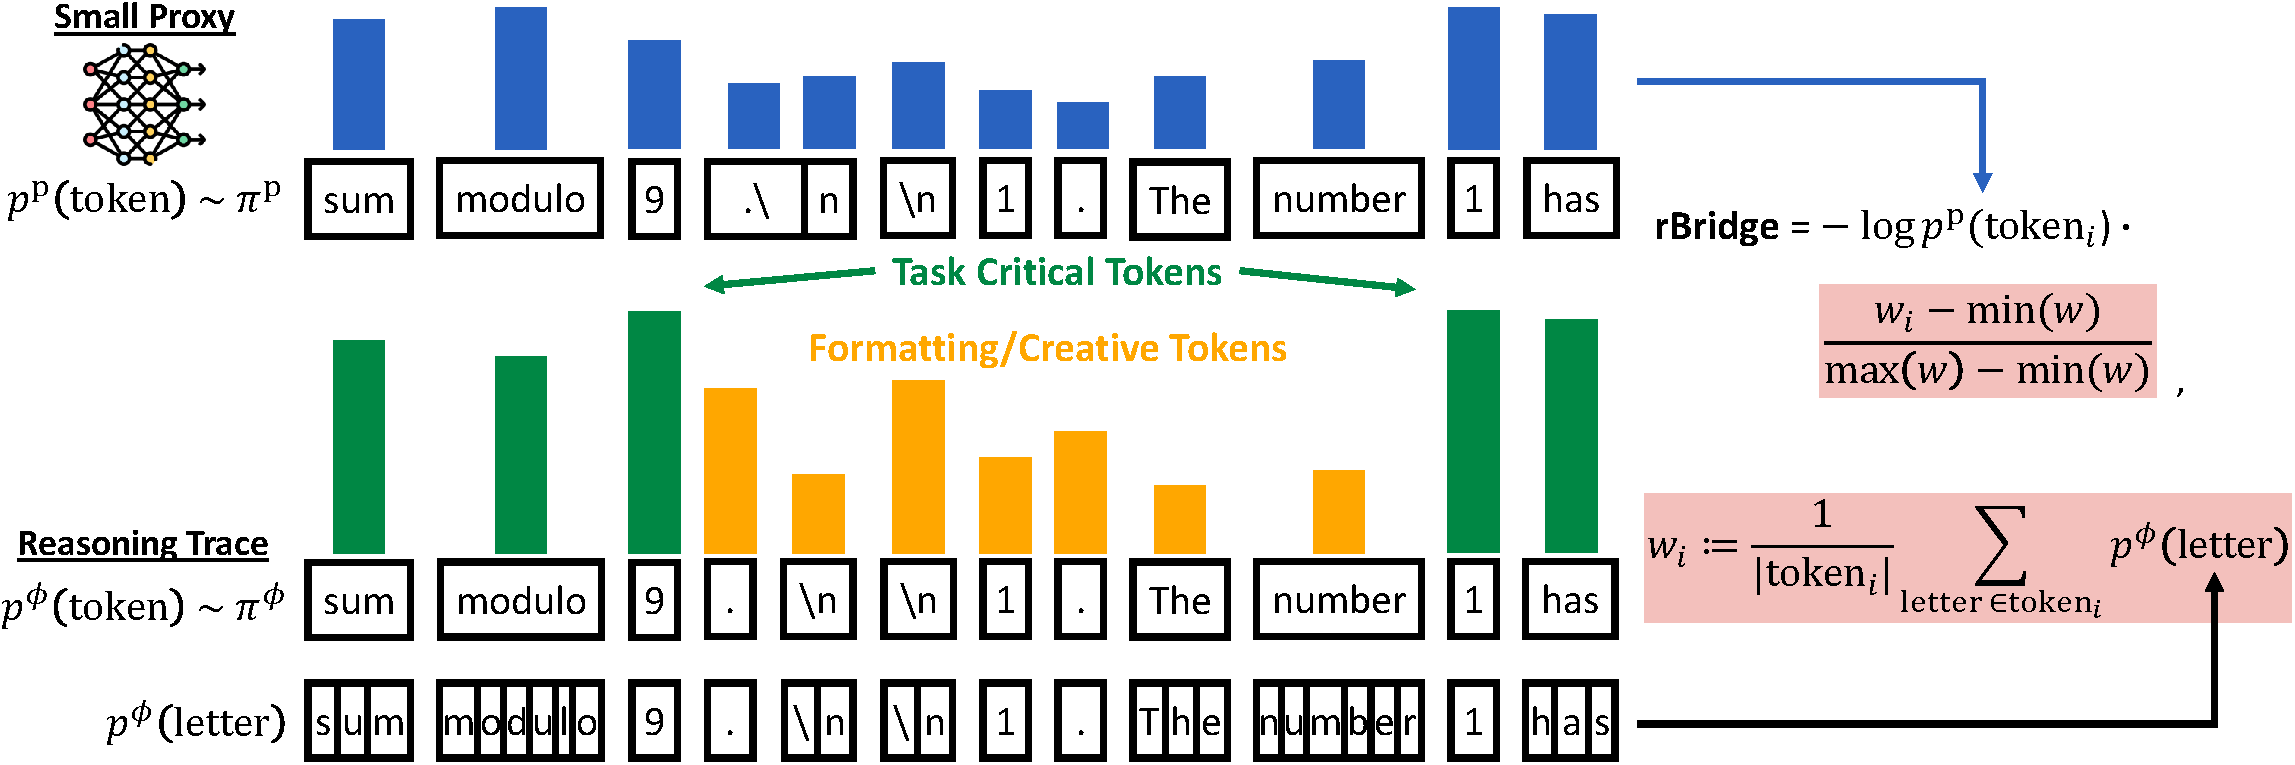
\includegraphics[width=\linewidth]{figs/rbridge3.pdf}
    \caption{Schematic overview of \tsc{rBridge}, which is used to predict and rank performance at much larger model size. We use a frontier model $\pi^\phi$'s reasoning trace \citep{NEURIPS2022_9d560961} as the gold label $Y^*$ and compute {\setlength{\fboxsep}{1pt}\colorbox{myred!30}{weighted}} NLL for evaluation. Each token $i$'s NLL is {\setlength{\fboxsep}{1pt}\colorbox{myred!30}{weighted}} by the frontier model's confidence in that token (MinMax normalized). To handle tokenizer mismatches between proxy and frontier models, we compute weights at the letter level and average within tokens.}
    \label{fig:rbridge}
\end{figure}

Pre-training modern language models at scale requires enormous computational and data resources, making it infeasible to exhaustively explore pre-training design choices directly at large scale \citep{radford2018improving, Radford2019, brown2020language, NEURIPS2019_c20bb2d9, hoffmann2022an,cottier2024rising,hu2024minicpm,khandelwal2024100,han2025trillion}. In response, leveraging smaller models as a proxy for larger model performance has been a key direction through the establishment of empirical scaling laws for prediction \citep{kaplan2020scaling,hoffmann2022training} or derivation of pre-training dataset rank invariance across scale \citep{magnusson2025datadecide}. 

However, the literature on the \textit{emergence} of reasoning performance as we scale model size \citep{wei2022emergent, almazrouei2023falcon, NEURIPS2024_5f1eee25} suggests that there may be a limit to how small theses proxy models can be. They demonstrate that reasoning capabilities only appear when models are sufficiently large in size. \citet{NEURIPS2024_5f1eee25}'s granular study demonstrates \textit{random} accuracy on small scale models of size 300M - 3B benchmarked on reasoning tasks like MMLU \citep{hendrycks2021measuring} and GSM8K \citep{cobbe2021training}. Contrarily, other non-reasoning benchmarks like TriviaQA \citep{joshi-etal-2017-triviaqa} and HellaSwag \citep{zellers-etal-2019-hellaswag} show smooth signs of improvement even at small scale. 

We further visualize this challenge of using small models to proxy large model especially for reasoning in Fig. \ref{fig:motivation}. While larger models exhibit stable Accuracy (Acc.) improvement (Fig. \ref{fig:13b32b}), smaller models are highly noisy, and in the case of the smallest 1B model, sloping in the wrong direction (Fig. \ref{fig:1b7b}).

%This challenge persists across mathematics, science, engineering, commonsense, and coding benchmarks visualized in in Appendix \ref{app:noisy}. \sungjun{Comment: unncessary I think.simply point to Appendix for details?}

Due to this limitation, practitioners are often constrained to relatively larger proxy models up to 15B to capture reasoning performance, which incurs substantial computational and economic costs \citep{grattafiori2024llama3herdmodels, deepseekai2025deepseekv3technicalreport}. For example, a single training run of a 7B model with 500B tokens can reportedly exceed 50K USD in cost \citep{han2025trillion}. 

% Alternatively, practitioners may resort to smaller models evaluated on smoothly scaling benchmarks \citep{liu2025regmix, xie2023doremi}, but they are suboptimal correlates of the target model's reasoning capabilities. 

\begin{figure}[tb]
    \centering
    \begin{subfigure}[b]{0.497\textwidth}
        \centering
        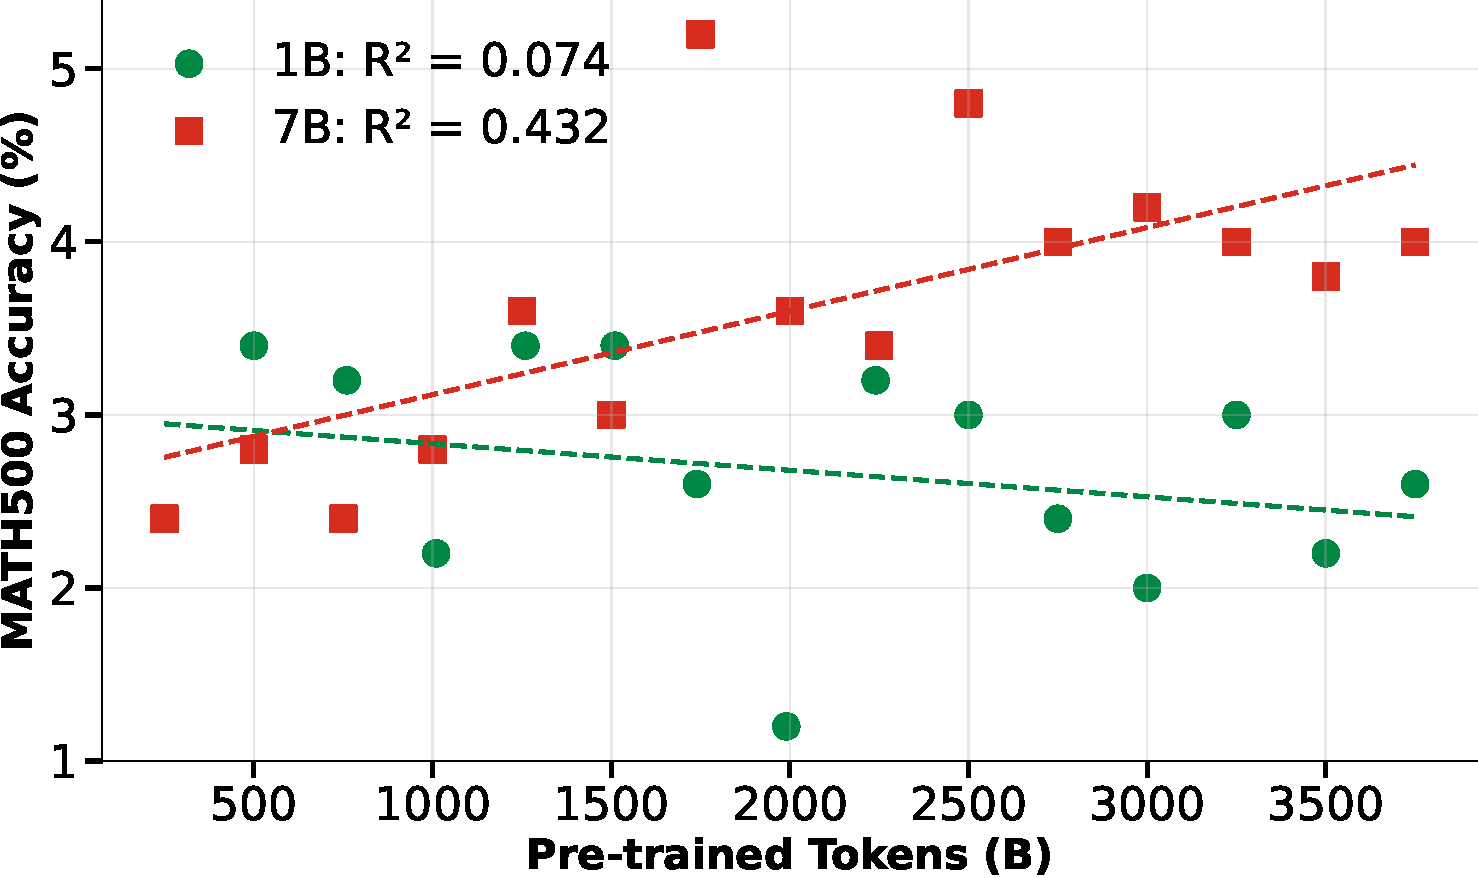
\includegraphics[width=\textwidth]{figs/math500_1b_7b_performance.pdf}
        \caption{Pre-training progress on 1B and 7B model}
        \label{fig:1b7b}
    \end{subfigure}
    \hfill
    \begin{subfigure}[b]{0.497\textwidth}
        \centering
        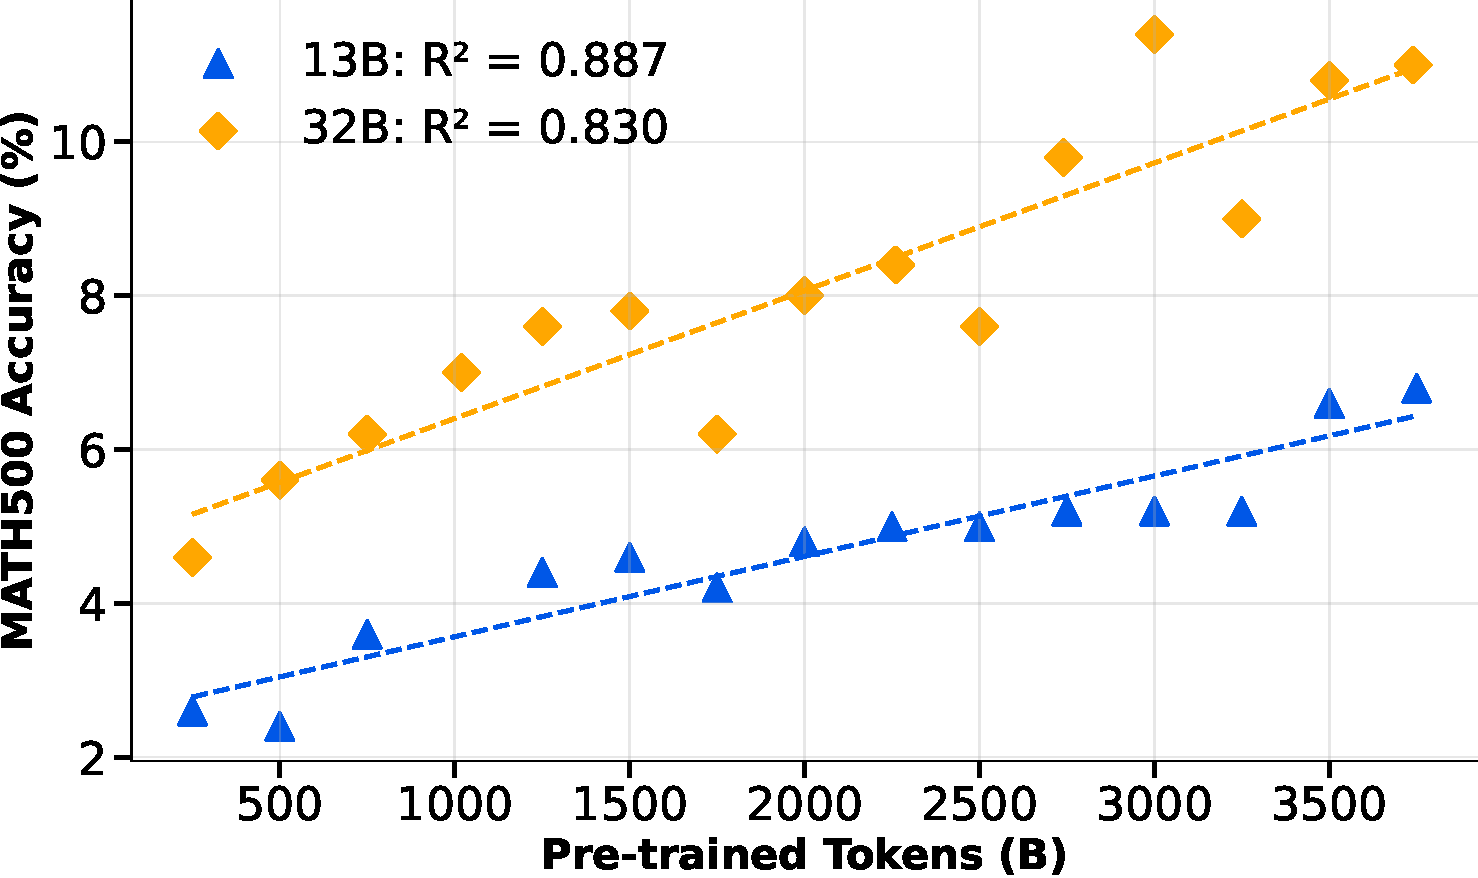
\includegraphics[width=\textwidth]{figs/math500_13b_32b_performance.pdf}
        \caption{Pre-training progress on 13B and 32B model}
        \label{fig:13b32b}
    \end{subfigure}
    \caption{Using MATH500 as an example benchmark, given the same data source OLMo-Mix-1124 \citep{olmo20242}, smaller models exhibit more noise and get the direction wrong, making it challenging to use smaller models to proxy larger model performance. R$^2$ values are derived from linear curve fitting. Extended visualization across other reasoning benchmarks are available in Appendix \ref{app:noisy}.}
    \label{fig:motivation}
\end{figure}

% To fill this literature gap, we raise the following research question: \textit{Can we effectively predict pre-trained large model's reasoning via small proxy model, and use these to rank datasets?}

% Our preliminary empirical studies analyzes indicate the limitation of standard negative log likelihood (NLL) and alternative innovations to the standard NLL.
 
\paragraph{Contribution.} To bridge the evaluation scheme at small proxy to large target scale, we first analyze limitations of past approaches (\textbf{\S\ \ref{sec:limit}}). Our analysis uncovers that existing methods fail to \textbf{(\S\ \ref{sec:limit} (1))} align with the pre-training objective, and \textbf{(\S\ \ref{sec:limit} (2))} align with the target task. \textbf{(1)} Alignment with the pre-training objective is required as small pre-trained models \textit{lack strong generalization capabilities}. \textbf{(2)} Ensuring that the evaluation scheme is aligned with the target task is necessary to fulfil our \textit{ultimate} goal of proxying task performance at large scale. To achieve \textbf{(1, 2)}, we use frontier-model generated gold reasoning traces \citep{NEURIPS2022_9d560961} for negative log-likelihood (NLL) (Fig. \ref{fig:rbridge}). Then, we further task alignment at the token-level by automatically weighting tokens based on their level of task-alignment (Fig. \ref{fig:rbridge}). We empirically validate our method \tsc{rBridge} (\textbf{\S\ \ref{sec:exp}}) in the following five ways:
\begin{enumerate}
    \item On a pre-training dataset ranking benchmark with target 1.2B scale, \tsc{rBridge} achieves \textbf{80.8\%} decision accuracy across \textbf{25} pre-training datasets, outperforming \textbf{5} baselines, reducing dataset ranking compute cost by at least \textbf{100.2$\times$} against the best .
    \item \tsc{rBridge} achieves best average proxy (1B) to target (13B, 32B) relationship across \textbf{6} benchmarks (mathematics, science, engineering, commonsense, and coding tasks), against \textbf{6} baselines. 
    \item \tsc{rBridge} achieves best average 1B $\rightarrow$ 13B relationship after a supervised fine-tuning (SFT) stage at target scale across \textbf{4} benchmarks, against \textbf{6} baselines.
    \item \tsc{rBridge} outperforms proxy models \textbf{7 - 13$\times$} larger using the target metric (e.g. Acc., Pass@K).
    \item Finally, we demonstrate that \tsc{rBridge}-target relationship on one pre-trained dataset can be \textbf{zero-shot transferred} to an alternative dataset for low-error performance prediction and ranking using a \textbf{fraction} of experimental compute cost.
\end{enumerate}

% Deprecated introduction

%For instance, \cite{xie2023doremi}, \cite{liu2025regmix} leverage proxy models (1 - 280M) to help optimize pre-training data mixture weights at target scale ($~$7B) operate under the notion that performance at very small scale have a meaningful relationship with larger scales \sungjun{Comment: I am afraid introducing this here might give the readers wrong idea that it is possible to optimize using very small proxy models targeting large models. My suggestion is to move this to a related work section where we can provide more details. I also mention the limitations of their method below in my text insert as well. }.

% A common strategy to mitigate this cost is to study proxy models: smaller models trained under constrained budgets to approximate how larger models might respond to different training conditions. These proxies enable systematic investigation of scaling behaviors while keeping experimentation tractable.

% Modern large language models' (LLMs) success can be largely attributed to the pre-training (self-supervised learning) and post-training paradigm \citep{radford2018improving, Radford2019, brown2020language, NEURIPS2019_c20bb2d9}. The large pre-training data size and corresponding model size allows for improved downstream performance and generalization \citep{groeneveld-etal-2024-olmo,isik2025scaling}. In this paradigm, pre-training notoriously consumes a significant amount of economic cost due to outsized compute costs \citep{hoffmann2022an,cottier2024rising,hu2024minicpm,khandelwal2024100,han2025trillion}. This high-cost problem is amplified as researchers search for optimal pre-training recipes \citep{NEURIPS2021_8df7c2e3}. 

% Therefore, it is unclear how reliable leveraging small proxy models ($\leq 1$B) to predict larger-scale target models is. \sungjun{Comment: with the above added context, we don't need this statement anymore - as we have strongly presented the case that <1B is just not reliable of larger target models}

% Past works utilize benchmarks that do not exhibit emergent behavior: \cite{xie2023doremi}, \cite{liu2025regmix}'s data mixture optimization study conducts experiments on non-emergent benchmarks like TriviaQA and HellaSwag \citep{NEURIPS2024_5f1eee25} \sungjun{Comment: Move this to a related work section.}.

% \begin{wrapfigure}{r}{0.4\textwidth} 
%   \vspace{-15pt}
%   \centering
%   \includegraphics[width=0.4\textwidth]{figs/diagram.pdf} 
%   \caption{High-level schematic diagram of evaluation scale transfer for pre-training.}\label{fig:diagram} 
%   \vspace{-5pt}
% \end{wrapfigure}

 % First, we empirically confirm that reasoning evaluation using the target metric (Accuracy or Pass@k) is highly noisy in smaller models (\textbf{\S\ \ref{sec:lack}}).

% \section{Preliminary: Problem Formulation and Notations} \label{sec:prelim} 
% --- juyoung's ---

% We consider the setting where the evaluation target is fixed: a large-scale model (the \textit{target}) is assessed on reasoning benchmarks using standard metrics such as Accuracy (Acc.) or Pass@k (p@k). Our goal is to leverage much smaller \textit{proxy} models—defined by $|\theta^\text{p}| < |\theta^\text{t}|$—to estimate how the target model would perform, without incurring the prohibitive costs of training and evaluating at full scale.  

% The challenge lies in designing a proxy \textit{evaluation scheme}. Directly applying the target metric to small proxies is unreliable: their scores are noisy and often fail to correlate with large-scale behavior, especially on reasoning benchmarks. Instead, we seek proxy metrics that provide stable and informative signals, enabling what we call \textit{evaluation scale transfer}.  

% Why is such transfer important? We highlight two key scenarios:  
% \begin{itemize}
%     \item \textbf{Intra-recipe transfer.} Practitioners often face the decision of whether to continue scaling a given training recipe. For example, doubling the training budget from 500B to 1000B tokens may incur enormous additional cost, but the expected gain in Accuracy or Pass@k is uncertain. A reliable proxy evaluation scheme would allow practitioners to anticipate these gains early with small models, helping decide whether further scaling is worthwhile.  
%     \item \textbf{Inter-recipe transfer.} Another common challenge is selecting among multiple candidate training data sources. Training large models on each option is prohibitively expensive, yet choosing the wrong dataset can waste vast resources. Here, proxies can act as lightweight evaluators, ranking datasets or mixtures before committing to full-scale runs.  
% \end{itemize}  

% --- juyoung's ---
% We consider the setting where the evaluation \textbf{t}arget is fixed: a large-scale pre-trained model $\pi^\text{\textbf{t}}$ assessed on reasoning benchmarks using Acc. or Pass@k (p@k). Our goal is to leverage much smaller \textbf{p}roxy model $\pi^\text{\textbf{p}}$ to estimate how the target model would perform at a significantly reduced compute cost. Concretely, we aim to search for a proxy metric, $\text{metric}^\text{p}$, which achieves the strongest relationship $f: \text{metric}^\text{p}( \pi^\text{p}) \mapsto \text{Acc./p@k}( \pi^\text{t})$. If we are interested in performance prediction, we can use Pearson Correlation R$^2$ \citep{benesty2009pearson} and Mean Absolute Error (MAE; \cite{chai2014root}). Alternatively, for ranking relationships we can use Decision Accuracy (DAcc.; \cite{magnusson2025datadecide}) and Kendall Tau \citep{sen1968estimates}. For succinctness in explaining experiment scale $n$ $\rightarrow$ $m$ denotes proxy model size $n$ to target model size $m$, e.g., 1B $\rightarrow$ 32B. For next token prediction we denote $p(y_\tau \vert x, y^*_{<\tau})$, where $y$ is the decoded token, $x$ is the prompt, and $\tau$ denotes token step.

% Intuitively, when we observe a change ($\Delta$) in proxy $\text{metric}^\text{p}$, we should be able to expect $\Delta\text{metric}^\text{t}$, if we derive a strong relationship, e.g., via Pearson Correlation \citep{benesty2009pearson} and Kendall Tau \citep{sen1968estimates}. As the target $\text{metric}^\text{t}$ is given as Accuracy (Acc.) or Pass@k (p@k), we aim to find a metric$^\text{p}$ that best proxies $\text{metric}^\text{t}$. We consider two cases that cause $\Delta\text{metric}^\text{t}$. \textbf{[1] Intra-recipe} $\Delta$: $\Delta$ caused by difference in training data size, e.g., training token size of 500B to 1000B commonly causes $\text{metric}^\text{t}$ to improve. Here, we assume that the pre-training data set source is equivalent across scale. The intra-recipe setting is used to predict performance at larger scale. \textbf{[2] Inter-recipe} $\Delta$: $\Delta$ caused by using a different training data source. The inter-recipe setting is used for pre-training dataset search (ranking). 


% as we acknowledge the challenge of exposure bias \citep{NIPS2015_e995f98d,ranzato2015sequence}, where next token prediction (1-token roll out) has a lower error bound over free-form generation ($n$-token roll out) as the gold context ($y^*_{<t}$) is provided. As discussed in the exposure bias literature, $n$-token roll outs used for Accuracy and Pass@k result in accumulated error.


% \input{sections/new_method}

\section{Problem Setting} \label{sec:problem}
Let $\pi^\text{p}, \pi^\text{t}$ denote small proxy and large target model, respectively. The target metric $\text{metric}^\text{t}$ (e.g., Acc., Pass@k) is fixed. Our objective is to design a proxy evaluation $\text{metric}^\text{p}$ such that considering $f: \text{metric}^\text{p} \mapsto \text{metric}^\text{t}$, find $\text{metric}^\text{p} := \max_{\text{metric}} \text{corr}(\text{metric}(\pi^\text{p}), \text{metric}^\text{t}(\pi^\text{t}))$. We discuss the corr($\cdot$) function we use in future sections. That is, improvements observed at proxy scale should reliably predict improvements at target scale. We denote scaling experiments as $n \rightarrow m$, where $n, m$ is the proxy, target model size, respectively; e.g., $1\text{B} \rightarrow 32\text{B}$. Performance changes can arise from either \textbf{(I)} varying the training dataset at fixed data size, or \textbf{(II)} varying the training data size given a fixed dataset. This enables two key applications: \textbf{(I)} comparing alternative training datasets without training large models on each, and \textbf{(II)} predicting whether scaling up training data (e.g., 3000B → 3500B tokens) is worthwhile. This is important because it enables us to predict the return on investment for large-scale training before committing resources. A practical proxy evaluation scheme must therefore be reliable at \textit{small scale} and achieve \textit{high correlation}.

% In turn, from a practical perspective, we aim to maximize $\text{relationship}(\text{metric}^\text{p}(\pi^\text{p}), \text{metric}^\text{t}(\pi^\text{t}))$ under two key scenarios: \textbf{(1)} Comparing alternative training datasets without training a large model on each option, \textbf{(2)} Predicting whether scaling up a given training dataset (e.g., 500B $\rightarrow$ 1000B tokens) is worthwhile. A practical proxy evaluation scheme must therefore be \textit{reliable at small scale} and \textit{transferable across training datasets}.

% In other words, we are attempting to solve the following optimization problem: $\max_{\text{metric}^\text{p}} \text{corr}(\text{metric}^\text{p}(\pi^\text{p}), \text{metric}^\text{t}(\pi^\text{t}))$. 

% Note that our definition of $\text{metric}^\text{p}$ also includes possible transformations of the underlying evaluation data of $\text{metric}^\text{t}$. 



% Training large reasoning models is prohibitively expensive. As a result, practitioners often rely on \textit{proxy models}—smaller, pre-train-only models—to anticipate the effectiveness of different pre-training recipes before committing resources to large-scale runs.  
% Formally, 

\section{Bridging Small and Large Model Scale Evaluation} \label{sec:rbridge}

\begin{figure}[tb]
    \centering

    \begin{subfigure}[b]{\textwidth}
        \centering
        
\includegraphics[width=0.5\textwidth]{figs/legend_graded.pdf}
        \label{fig:legend}
    \end{subfigure}

    \begin{subfigure}[b]{0.497\textwidth}
        \centering
        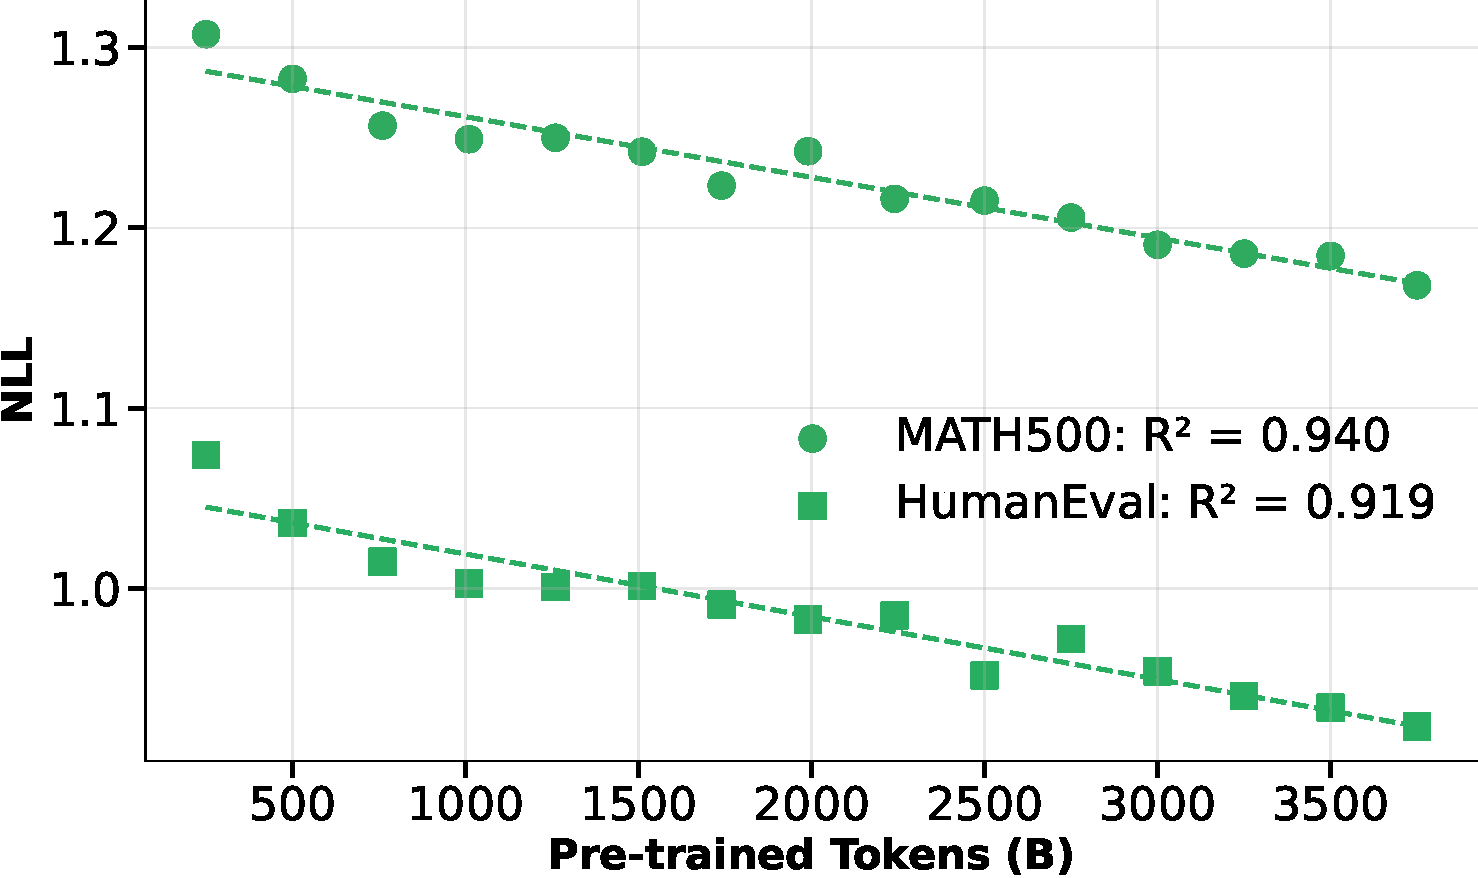
\includegraphics[width=\textwidth]{figs/low_ll_benchmarks.pdf}
        \caption{In-distribution $Y^*$ provides smooth signal.}
        \label{fig:id}
    \end{subfigure}
    \hfill
    \begin{subfigure}[b]{0.497\textwidth}
        \centering
        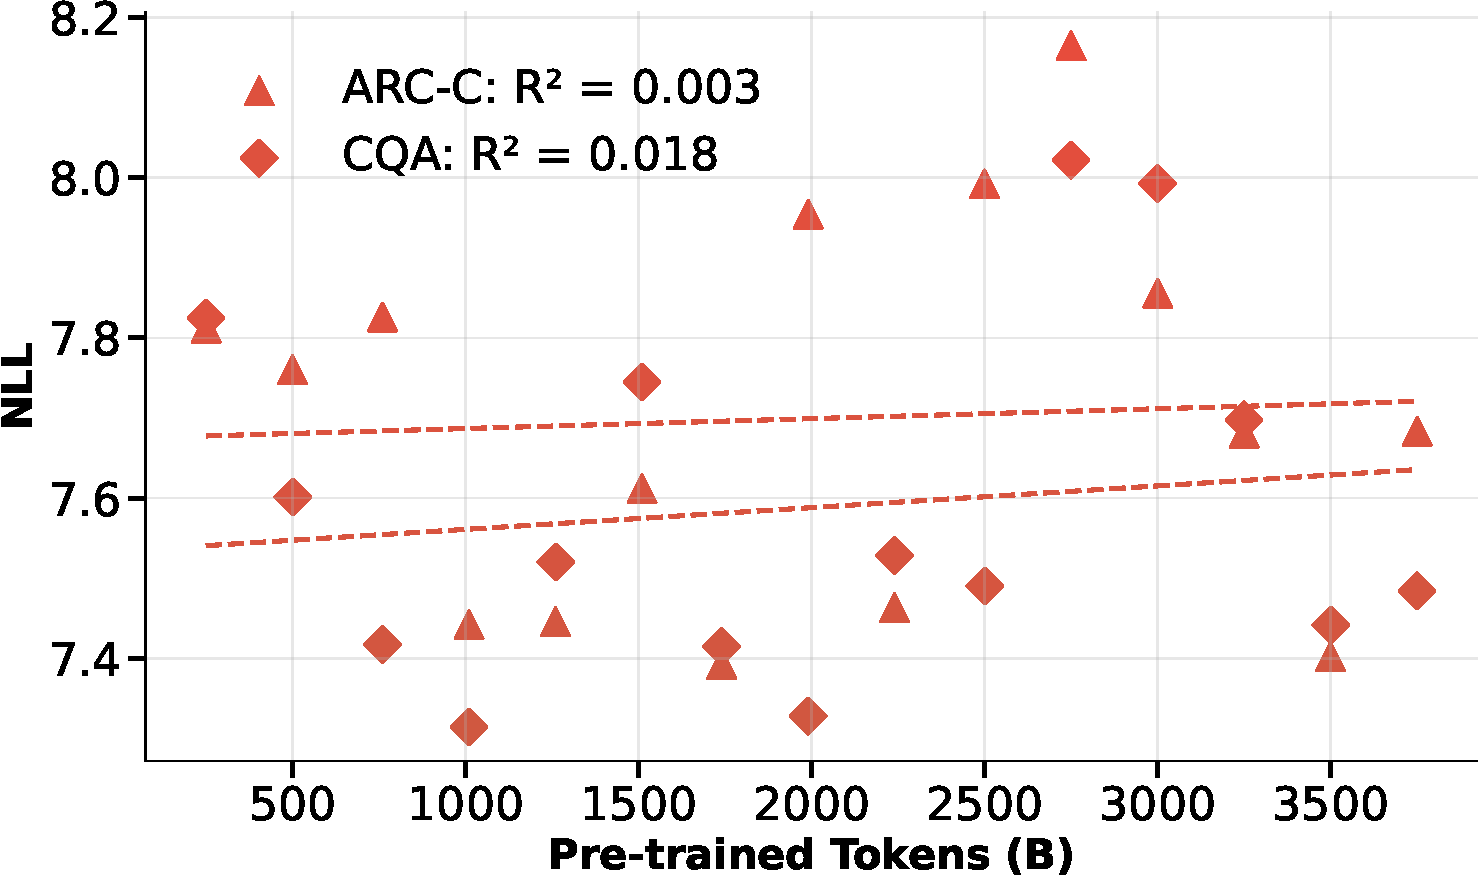
\includegraphics[width=\textwidth]{figs/high_ll_benchmarks.pdf}
        \caption{Out-of-Distribution $Y^*$ provides no signal.}
        \label{fig:ood}
    \end{subfigure}
    \caption{When evaluating a 1B pre-trained model with next token prediction, $\pi^\text{p}(y_\tau \vert x, y^*_{<\tau})$, whether the target $Y^*$ is in-distribution becomes important. All visualized benchmarks demonstrate smooth improvements at larger (13$\times$, 32$\times$) scale with target metric Acc./p@k. For clarity, we visualize the benchmarks in our empirical study with the two smallest and largest average NLL values.}
    \label{fig:idood}
\end{figure}
We find that small models become strong proxies for large models when achieving alignment along two axes: alignment with the pre-training evaluation objective \textbf{(\S\ \ref{sec:limit} (1))}, and alignment with the target task \textbf{(\S\ \ref{sec:limit} (2))}. In response, we introduce our method, \tsc{rBridge} \textbf{(\S\ \ref{sec:align})}.

\subsection{Prior Approach Limitation}\label{sec:limit}

\paragraph{(1) Evaluation Objective Misalignment.} We find that the first limitation of existing approaches is their lack of evaluation objective alignment with $\pi^\text{p}$. This is required as small pre-trained models \textit{lack strong generalization capabilities}. Concretely, \textbf{(a)} Acc. and Pass@K (p@k) is misaligned with the pre-training objective function, and \textbf{(b)} even if we use an objective function aligned evaluation scheme like NLL, we must stay aligned with the pre-trained model's distribution. 

\paragraph{(1.a) Misaligned Evaluation Metric.} Existing target metrics like Acc./p@k are misaligned with the proxy model's next token prediction (NTP) NLL learning objective \citep{brown-etal-1992-class}. \begin{center}
\vspace*{-6mm}

    \begin{minipage}[b]{0.497\textwidth}
        \centering
        \resizebox{\textwidth}{!}{
        \begin{tabular}{lccc}
        \toprule
        \textbf{$Y^*$:} & $\mathcal{D}$ & \textbf{ScB = $R^\phi$ + $A^\phi$}  & \textbf{$R^\phi$} \\
        \midrule
        Min NLL ($\downarrow$)   &\cellcolor{myorange!30} 1.168 & \cellcolor{myred!30} 1.285 & \cellcolor{mygreen!30} 0.925 \\
        Average NLL ($\downarrow$)   &\cellcolor{myorange!30} 1.228 & \cellcolor{myred!30} 1.351 & \cellcolor{mygreen!30} 0.981 \\
        Max NLL ($\downarrow$)   &\cellcolor{myorange!30} 1.307 & \cellcolor{myred!30} 1.405 & \cellcolor{mygreen!30} 1.060 \\
\multicolumn{4}{c}{\cellcolor{gray!10}\textbf{1B $\rightarrow$ 13B}}\\
        Train $R^2$ ($\uparrow$) &\cellcolor{myorange!30}0.861 & \cellcolor{myred!30}0.814 & \cellcolor{mygreen!30}0.886 \\
        Test MAE ($\downarrow$)   & \cellcolor{myorange!30}0.593 & \cellcolor{myred!30}0.637 & \cellcolor{mygreen!30}0.524 \\
\multicolumn{4}{c}{\cellcolor{gray!10}\textbf{1B $\rightarrow$ 32B}}\\
        Train $R^2$ ($\uparrow$) & \cellcolor{myorange!30}0.823 & \cellcolor{myred!30}0.809 & \cellcolor{mygreen!30}0.832 \\
        Test MAE ($\downarrow$)   & \cellcolor{myorange!30}0.815 & \cellcolor{myred!30}0.933 & \cellcolor{mygreen!30}0.739 \\
        \bottomrule
        \end{tabular}
        }
        \captionof{table}{We observe a direct relationship between degree of in-distribution (as presented as NLL) and performance. Best to worst in each row labeled as {\setlength{\fboxsep}{2pt}\colorbox{mygreen!30}{green} \colorbox{myorange!30}{orange}, \colorbox{myred!30}{red}.}} \label{tab:scb}
    \end{minipage}
    \hfill 
    \begin{minipage}[b]{0.497\textwidth}
        \centering
        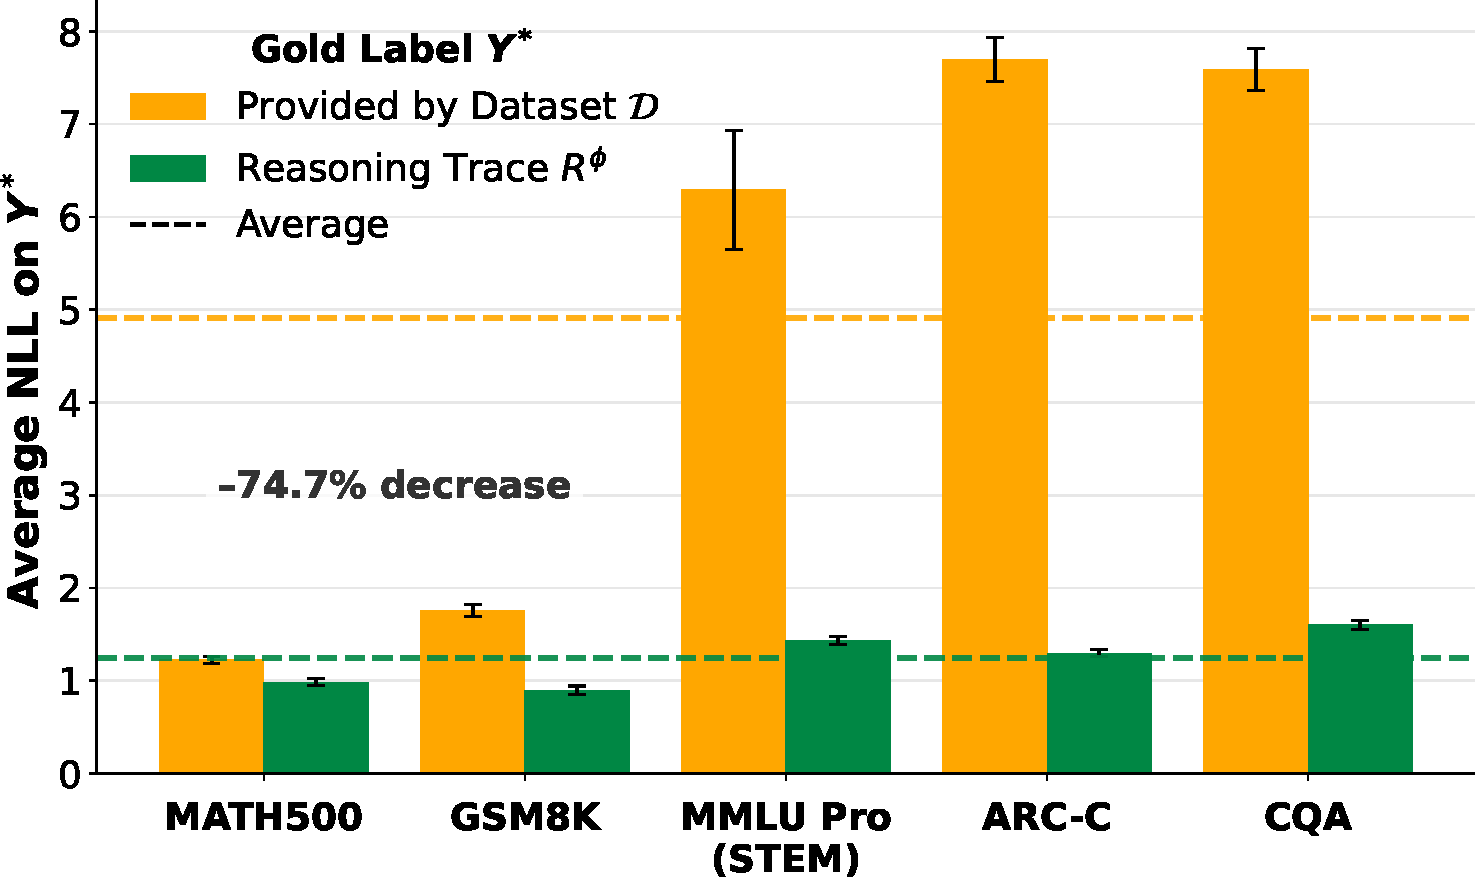
\includegraphics[width=\textwidth]{figs/ll_decrease.pdf}        
        \captionof{figure}{Using reasoning trace $R^\phi$ over benchmark test set's $Y^*$ significantly reduces NLL, suggesting that $R^\phi$ is more in-distribution. Error bars indicate one standard deviation.}\label{fig:scb_clean}
    \end{minipage}
\end{center}
\vspace*{-1mm}Consider Fig. \ref{fig:id}, where NLL shows smooth improvement with correct slope at 1B on MATH500 while Acc. in Fig. \ref{fig:motivation} is noisy and sloping the wrong direction.

\paragraph{(1.b) Not All NLL are Equal: Distributional Alignment.} Furthermore, we find that the quality of the NLL signal hinges on the gold label $Y^*$. We define gold label as the string used for NLL on our proxy model. We observe that it should be closer to the pre-training distribution $p(y_\tau \vert x, y^*_{<\tau}) \sim \pi^\text{p}$ where $x$ is the input, and $\tau$ is the decoded token. Following \cite{arora-etal-2021-types}, \cite{gonen2023demystifying}, we measure how in-distribution (ID) $Y^*$ is via NLL, $-\log(p(Y^*))$. The more out-of-distribution (OOD), the more lacking in signal the proxy model becomes (Fig. \ref{fig:idood}). Benchmarks with an ID $Y^*$ (lower NLL) show smooth and predictable progress at smaller model scale (1B) (Fig. \ref{fig:id}). Contrarily, benchmarks with OOD $Y^*$ (higher NLL) is at least as noisy as the target metric Acc. (Fig. \ref{fig:ood}). 

We also observe this distributional misalignment in ScalingBench (ScB; \cite{xiao2024densing,team2025minicpm4}). ScB proposes we set the reasoning trace $R^\phi$ \citep{NEURIPS2022_9d560961} and the final answer label $A^\phi$ of a frontier model $\pi^\phi$ as $Y^*$. ScB's gold labels include formatting artifacts like ``$\backslash$n", ``Final Answer:", and ``I hope it is correct." that rarely appear in pre-training data, making them OOD, hurting proxy performance (Tab. \ref{tab:scb}). The proxy evaluation protocol is detailed in \textbf{\S\ \ref{sec:protocol} (ii)}. 

% For instance, in ScB's MATH $Y^*$ their final answer label is includes ``$\backslash$n", ``Final Answer:", and ``I hope it is correct." which does not commonly occur in the pre-training corpora. Therefore, in the case of ScB provided MATH $Y^*$, the NLL is more OOD (Tab. \ref{tab:scb}). Our preliminary study shows that this hurts proxy performance (Tab. \ref{tab:scb}).

\paragraph{(2) Target Task Alignment of Gold Label $Y^*$ and at the Token Level.} Secondly, we hypothesize that the evaluation scheme should be task aligned. Here, target task refers to, e.g., correctly solving math problems for GSM8K \citep{cobbe2021training}, and MATH500 \citep{hendrycks2021math}. Ensuring that $Y^*$ is aligned with the target task is necessary to fulfilling our \textit{ultimate} goal of proxying task performance at large scale. While we could achieve maximal ID by setting the greedy decoded tokens of $\pi^\text{p}(y_\tau \vert x, y^*_{<\tau})$ as $Y^*$, this would provide no signal, as it would fail to be task aligned. 

We further observe that standard NLL on $Y^*$ does not distinguish between tokens that are important for task alignment, and others that are less task critical. Consider, Fig. \ref{fig:rbridge}, where frontier model $\pi^\phi$ decoding produces both {\color{mygreen}\textbf{task critical}} and {\color{myorange}\textbf{formatting/creative}} tokens. For example, newlines and numbering are not essential, while steps like ``sum modulo 9’’ are crucial. To further achieve task alignment, tokens should not be arbitrarily given equal weight as is in NLL. 

\subsection{rBridge: Improving Evaluation Objective Alignment and Task Alignment} \label{sec:align}
  
\paragraph{Reasoning Trace $R^\phi$ as $Y^*$.} We show that using only the reasoning trace $R^\phi$ of a frontier model $\pi^\phi$ as $Y^*$ satisfies both being \textbf{(1)} ID and \textbf{(2)} task alignment. \textbf{(1)} We hypothesize that $R^\phi$ is more distributionally aligned (ID) with the pre-training distribution comprised predominantly of a collection of continuous long texts \citep{NEURIPS2024_370df50c,kydlicek2025finepdfs}. We verify this empirically in Fig. \ref{fig:scb_clean}, where we visualize average NLL across 250 to 3750B trained tokens on a 1B model, on the provided $Y^*$ by the benchmark dataset $\mathcal{D}$ against the frontier model $\pi^\phi$ generated $R^\phi$. We observe an average NLL decline of 74.7\% when using $R^\phi$ across five reasoning benchmarks, providing supportive evidence that $R^\phi$ is more ID. \textbf{(2)} $R^\phi$ is well aligned with the target task as $R^\phi$ is the reasoning trace that leads to the correct final answer for Acc./p@k. Intuitively, evaluating how well the model $\pi^\text{p}$ reasons towards the final answer is a good ID proxy for achieving the target Acc./p@k. Empirically, using only $R^\phi$ achieves the best relationship on MATH500 which we are able to replicate as the exact ScB $Y^*$ gold labels have been released for MATH500 (Tab. \ref{tab:scb}).  

 % We wish to refine $Y^* := R^\phi$ automatically so that tokens that are more task aligned are given more weight.

\paragraph{Weighted NLL on $R^\phi$'s Tokens for 
Further Task Alignment.} \tsc{rBridge} takes a final step for further task alignment by weighting each token by its level of task-alignment. We hypothesize that frontier model token probability $p^\phi(\text{token}_i) \sim \pi^\phi$ provide automatic task-alignment weights:

\begin{equation}\label{eq:rbridge_nll}
    \text{\tsc{rBridge} NLL}(\text{token}_i):=  \underbrace{-\text{log}(p^\text{p}(\text{token}_i))}_{\text{standard NLL}} \cdot 
    \underbrace{\frac{1}{\vert \text{token}_i \vert} \sum_{\text{letter} \in \text{token}_i} p^\phi(\text{letter})}_{\text{Automatic tokenizer-agnostic task-alignment weight}
    }.
\end{equation}

Our method weighs each token $i$'s NLL by the frontier model's confidence in that token $p^\phi(\text{token}_i)$. To handle different tokenizers, we average letter-level probabilities within each token. Finally, we apply MinMax normalization \citep{witten2002data} on the weight factor in Eq. (\ref{eq:rbridge_nll}) to amplify the effect. Consider Fig. \ref{fig:rbridge} for an intuitive visualization of Eq. (\ref{eq:rbridge_nll}) with the MinMax normalized form unpacked in full. The pseudocode and prompt is available at Appendix \ref{app:pseudocode}.

% Finally, to amplify the effect of the task-alignment weight, we MinMax normalize \citep{witten2002data} it. We found this useful as $p^\phi(\text{token})$, and in turn $p^\phi(\text{letter})$ values taken via greedy decoding \citep{NIPS2014_5a18e133} naturally lead to probability distribution skewed towards high values. The pseudocode and prompt is available at Appendix \ref{app:pseudocode}.

% Note that we use their few-shot prompting format to evaluate NLL.

% In short, we evaluate performance using $K$-Fold Train $R^2$ and Test MAE.

% Such extreme non-task aligned $Y^*$ would provide the equivalent NLL across all scenarios. 

%as using free-form generation-based metrics like Acc. and pass@k leads to worse performance as error accumulates \citep{NIPS2015_e995f98d,ranzato2015sequence}. Intuitively, NTP is a more forgiving metric for the weak proxy model $\pi^\text{p}$ as at each decoding step $t$, the provided context $<t$ is the gold answer. We denote gold label for NTP as $Y^*$.

% We first overcome the inherent weakness of proxy models, being small and pre-train-only, by aligning the evaluation scheme with the pre-training objective. While larger models embody emergent behavior, i.e., achieving stable reasoning performance scores, we find that the best way to achieve reliable signals at small scale is by using the same metric the proxy pre-trained model $\pi^\text{p}$ was trained on. Therefore, we employ next token prediction (NTP) evaluation via average negative log likelihood per token (henceforth referred to as NLL; \cite{brown-etal-1992-class}). 

% We retrieve $R^\phi$ by prompting $\pi^\phi$ to generate a reasoning trace $R^\phi$ and final answer $A^\phi$. We discard $A^\phi$ and set $Y^* := R^\phi$.

% We qualitatively observe why benchmarks like ARC-C and CQA's $Y^*$ are significantly more OOD. As these benchmarks are multiple-choice question-based, the target $Y^*$ becomes the multiple-choice symbol, e.g., ``B" \citep{eval-harness}, or a short string, e.g. ``The Sun makes heat." \citep{gu-etal-2025-olmes}. In turn, $Y^*$ is distant from the pre-trained distribution of $\pi^\text{p}(y_\tau \vert x, y^*_{<\tau})$. Intuitively, as the pre-training corpora is predominantly a collection of continuous long texts \citep{NEURIPS2024_370df50c,kydlicek2025finepdfs}, such question-and-short-answer formats are rare in the corpora. 

% allowing the weight factor range to transform from $[a, b]$ to $[0, 1]$ where $a\geq0$ and $b\leq1$. min($\cdot$) and max($\cdot$) search space is set to the entire test set's evaluated tokens. 

% Straightforward assignment $p^\phi(\text{letter}) := p^\phi(\text{token})$, where letter $\in$ token, provides letter-level weights from the frontier-level model $\pi^\phi$. Letter-level is the most reasonable choice as this is the atomic unit of a token; meaning, we can re-map $p^\phi(\text{letter})$ back to any different tokenizer's token. As seen in Eq. \ref{eq:rbridge_nll}, this is achieved by finding the mean $p^\phi(\text{letter})$  across all letters composing the token. This weight factor is bounded by $[0, 1]$. A concretely example is visualized in Fig. \ref{fig:rbridge}.
% \paragraph{[2] Inter-dataset $\Delta$.} For inter-dataset $\Delta$ we employ Decision Accuracy (DAcc.; \cite{magnusson2025datadecide}), and Kendall's Tau. DAcc. is an evaluation metric proposed by \cite{magnusson2025datadecide} to quantify the proportion of all possible dataset pairs that are ranked correctly. We use DataDecide \citep{magnusson2025datadecide}, an open-source and -weight benchmark that studies inter-dataset ranking at a small scale of a $n\rightarrow$1.2B. We rank 25 different pre-training datasets using proxy models ranging in size $n \in [3.7\text{M},97.9\text{M}]$. We are unable to use challenging reasoning benchmarks like MATH500 and MMLU Pro as they exhibit significant noise at target scale of 1.2B. Therefore, we use ARC-C and CQA which shows stable cloze form (CF) accuracy \citep{gu-etal-2025-olmes} when averaging 3 seed pre-training runs \citep{gu-etal-2025-olmes}. All results are averages of the two benchmarks. 

% \paragraph{[2] Baselines.} We include five metrics that have been used by existing literature to select pre-training datasets using smaller proxy models: Correct Probability, Normalized Correct Probability, Total Probability, Margin, and 
% CF Accuracy \citep{xie2023doremi, liu2025regmix, magnusson2025datadecide}.

% Our experiments are divided into the following two categories \textbf{[1, 2]} with $n$ $\rightarrow$ $m$ denoting proxy model size $n$ to target model size $m$ where $n, m \in \mbb{N}^+$. Our main experiment is examining \textbf{[1]} intra-dataset $\Delta$ as for \textbf{[2]} inter-dataset $\Delta$, it is highly costly to pre-train $d \in \mbb{N}^+$ number of pre-training datasets at target model size of e.g., 13B, 32B. \textbf{[1]} remains computationally managable as only one target model has to be pre-trained. For \textbf{[2]}, we conduct experiments on a smaller target scale of 1.2B to demonstrate \tsc{rBridge}'s effectiveness in pre-training dataset ranking. 

% \begin{wrapfigure}{r}{0.45\textwidth} 
%   \vspace{-10pt}
%   \centering
%   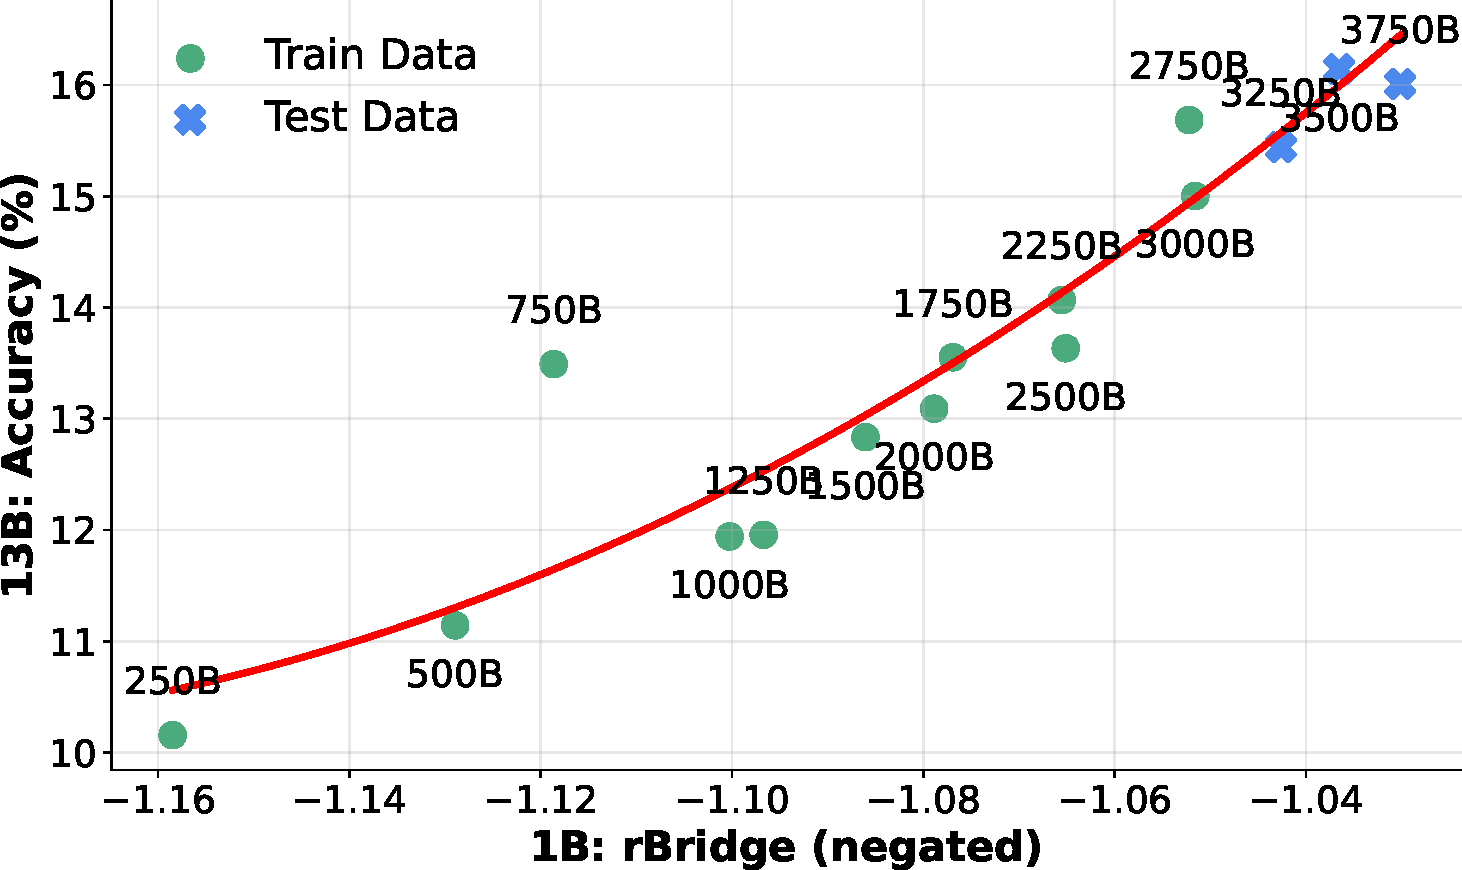
\includegraphics[width=0.45\textwidth]{figs/intra_example.pdf} 
%   \caption{Example visualization of the Intra-dataset $\Delta$ empirical study. This example is on one of the folds evaluating MMLU Pro (STEM).}\label{fig:intra_example} 
%   \vspace{-5pt}
% \end{wrapfigure}

% We examine how well a change in the target scale's Acc. or Pass@K induced by a change in training data size can be predicted by a change of metric value at proxy scale. We set-up the experiments so that the x-axis is a metric at proxy scale, and the y-axis is the target scale's Acc. or Pass@K. Each data point in this relationship corresponds to a certain amount of training data. The data source must be equivalent. See Fig. \ref{fig:intra_example} for an intuitive visualization. To evaluate the effectiveness of the relationship, we employ $5$-fold cross validation following \cite{che2018recurrent}, \cite{lee2020biobert}. Across 5-folds, we report the average curve fitting relationship R$^2$ on the train set and test Mean Absolute Error (MAE; \cite{chai2014root}). 

% We study 1B $\rightarrow$ 13B, and 1B $\rightarrow$ 32B with pre-trained tokens ranging 250 - 3750B tokens with evaluations in intervals of 250B tokens. The pre-training dataset is OLMo-Mix-1124 \citep{olmo20242}. We select six representative reasoning benchmarks spanning mathematics, science, engineering, commonsense, and coding: GSM8K, MATH500, ARC-C \citep{clark2018think}, MMLU Pro \citep{wang2024mmlupro} (STEM subset), CQA \citep{talmor-etal-2019-commonsenseqa}, and HumanEval \citep{chen2021evaluating}.

% We compare six alternatives: Accuracy/Pass@1 (target metric baseline; \citealp{NEURIPS2019_7298332f}), iSFT (intermediate supervised fine-tuning; \citealp{snell2024predicting}), Token Edit Distance (TED; discontinuity-based; \citealp{NEURIPS2023_adc98a26}), Model Probability of Correct Answer (MPCA; continuous, \citealp{NEURIPS2023_adc98a26, snell2024predicting}), and $R^\phi$ (our improved version of ScB; see \textbf{\S\ \ref{sec:align}}).


\section{Empirical Study}\label{sec:exp}

Our experiments are organized in three stages: \textbf{(i)} first, we show that \tsc{rBridge} can be used to rank datasets from proxy scale of $<$100M to target scale 1.2B, \textbf{(ii)} next, we examine the \tsc{rBridge}-target relationship across different amounts of training data at 1B to 32B scale, and \textbf{(iii)} finally, demonstrate that the relationship derived in \textbf{(ii)} can be effectively transferred to a different dataset, allowing us to predict \textit{and} rank large-scale datasets' reasoning performance at a fraction of the cost. 

% Our experiments are organized in three stages: \textbf{(i)} we demonstrate that \tsc{rBridge} effectively ranks datasets using proxy models ($<$100M parameters) to predict performance at target scale (1.2B parameters), \textbf{(ii)} we characterize the \tsc{rBridge}-target relationship across varying training data amounts at 1B--32B scale, and \textbf{(iii)} we show that relationships derived in \textbf{(ii)} transfer zero-shot to different datasets, enabling prediction and ranking of large-scale reasoning performance at substantially reduced computational cost.

\subsection{Experimental Protocol}\label{sec:protocol}

All experimental settings are set \textit{a priori}, and all methods are evaluated in the same manner. Detailed experimental details are available in Appendix \ref{app:setting}.

% \textbf{(i) Dataset Ranking at $<$100M $\rightarrow$ 1.2B.} 
% We follow DataDecide’s \citep{magnusson2025datadecide} protocol to test whether the \tsc{rBridge} score can effectively rank pre-training datasets. Specifically, we rank 25 datasets using proxy models and check whether these rankings align with the target model. Effectiveness is measured by Decision Accuracy (DAcc.; fraction of correctly ordered dataset pairs \citealp{magnusson2025datadecide}) and Kendall’s Tau.

\paragraph{(i) Dataset Ranking at $<$100M $\rightarrow$ 1.2B.} We evaluate whether \tsc{rBridge} scores from proxy models can effectively rank pre-training datasets for target model performance. Following DataDecide's protocol \citep{magnusson2025datadecide}, we rank 25 datasets using proxy models and assess alignment with target model rankings. We measure effectiveness using Decision Accuracy (DAcc.; fraction of correctly ordered dataset pairs; \cite{magnusson2025datadecide}) and Kendall's Tau correlation. Compute cost is measured as FLOPs = $6ND$, where $N$ is model size, and $D$ is dataset size, following \cite{kaplan2020scaling}.

\textbf{Setup.} Proxy models range $n \in [3.7\text{M}, 97.9\text{M}]$, with a 1.2B target model. As discussed in \textbf{\S\ \ref{sec:intro}}, noisy benchmarks such as MATH500 and MMLU Pro are excluded at this scale. Instead, we use ARC-C \citep{clark2018think} and CQA \citep{talmor-etal-2019-commonsenseqa}, which yield stable cloze-form (CF) accuracy \citep{gu-etal-2025-olmes} when averaged across three pre-training seeds \citep{magnusson2025datadecide}. Reported results are the average over these two benchmarks.
\begin{figure}[tb!]
    \centering
    \begin{subfigure}[b]{0.497\textwidth}
        \centering
        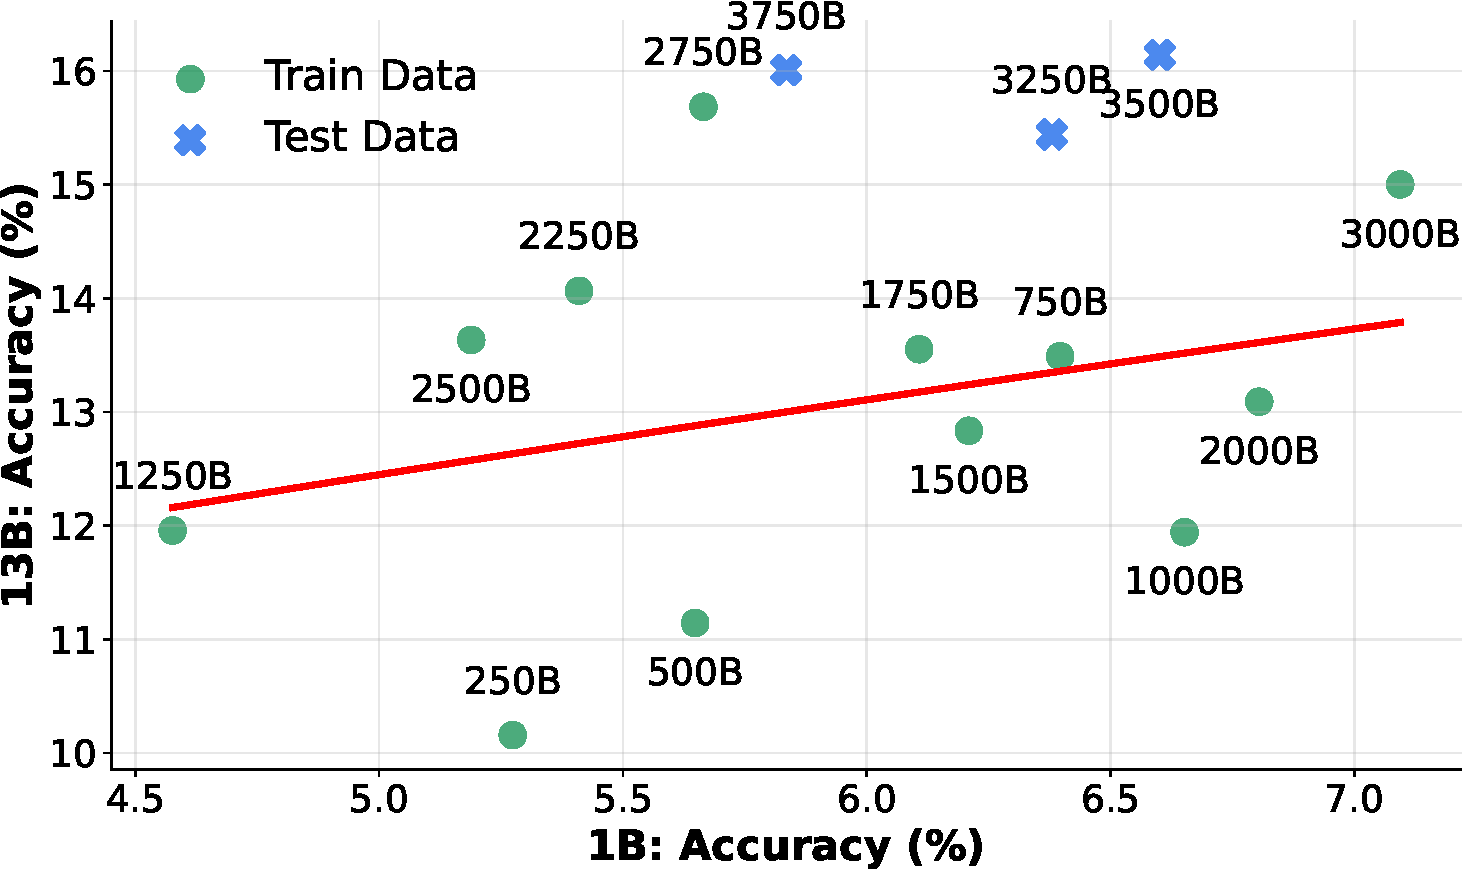
\includegraphics[width=\textwidth]{figs/intra_example_acc.pdf}
        \caption{Target metric Acc. as the proxy metric at 1B.}
        \label{fig:example_acc}
    \end{subfigure}
    \hfill
    \begin{subfigure}[b]{0.497\textwidth}
        \centering
        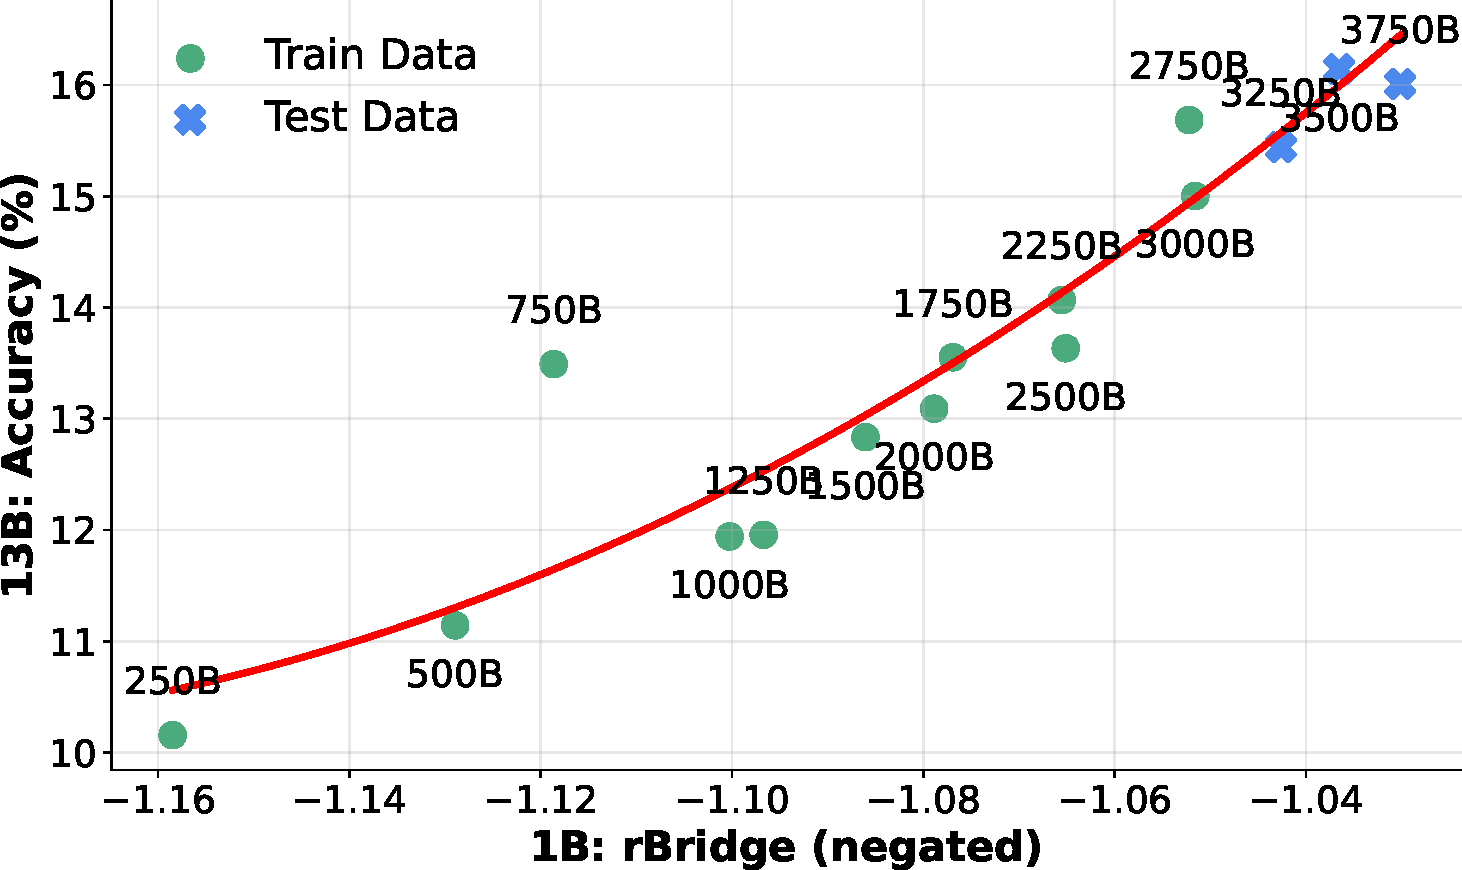
\includegraphics[width=\textwidth]{figs/intra_example.pdf}
        \caption{\tsc{rBridge} as the proxy metric at 1B.}
        \label{fig:example_rbridge}
    \end{subfigure}
    \caption{Example visualization from a fold of proxy-target relationship study at 1B $\rightarrow$ 13B on MMLU Pro (STEM). Each data point represents equal trained tokens for the proxy and target model. Extended visualizations for all other benchmarks available in Appendix \ref{app:more_exp}.}
    \label{fig:intra_example}
\end{figure}

\textbf{Baselines.} Alongside \tsc{rBridge}, we compare five \textit{dataset-ranking} metrics commonly used with proxy models: Correct Probability, Normalized Correct Probability, Total Probability, Margin, and CF Accuracy \citep{xie2023doremi, liu2025regmix, magnusson2025datadecide}.

\paragraph{(ii) Proxy-target Relationship Across Different Amounts of Training Data at 1B $\rightarrow$ 32B.} 

We test whether proxy-scale metrics can predict changes in target-scale Acc. and p@k across different training data sizes. Each data point corresponds to a specific data size from the same source (Fig.~\ref{fig:intra_example}). Following \cite{che2018recurrent}, \cite{lee2020biobert}, we evaluate using 5-fold cross validation on the setup visualized in Fig.~\ref{fig:intra_example}, reporting average train $R^2$ and test Mean Absolute Error (MAE; \cite{chai2014root}). Curve fitting selects the best function based on train $R^2$ from our hypothesis space: linear, quadratic, exponential, and logarithmic. This hypothesis space was defined \textit{a priori} to avoid overfitting. FLOPs 

\textbf{Setup.} We examine model scales of 1B $\rightarrow$ 13B and 1B $\rightarrow$ 32B, pre-trained on 250B to 3750B tokens in 250B token intervals using the OLMo-Mix-1124 dataset \citep{olmo20242}. Evaluation spans six reasoning benchmarks: GSM8K, MATH500, ARC-C, MMLU Pro (STEM subset; \cite{wang2024mmlupro}), CQA, and HumanEval \citep{chen2021evaluating}.

\textbf{Baselines.} We cover six alternative metrics that examine the relationship of small and large models given the \textit{same} data source, and metrics that have shown non-emergent continuity at small scale. First, we include the most naïve approach, the target metric: Accuracy and Pass@1 (Acc./p@1; \cite{NEURIPS2019_7298332f}). Second, we include intermediate supervised fine-tuning (iSFT; \cite{snell2024predicting}) which demonstrates that including a SFT stage throughout the intermediate pre-training checkpoints helps target metric (Acc./p@1) be used as signals. Third is Token Edit Distance (TED; \cite{NEURIPS2023_adc98a26}) which argue that emergence occurs due to discontinuous metrics, and correspondingly proposes their continuous metric. Fourth is Model Probability of Correct Answer (MPCA) as demonstrated in \cite{NEURIPS2023_adc98a26}, \cite{snell2024predicting} as a continuous metric. Last is ScB which visualizes the relationship between ScB and target metric using \textit{numerous} smaller proxy models (similar to the scaling law literature). As mentioned in \textbf{\S\ \ref{sec:rbridge}}, we use our proposed improved version of ScB, R$^\phi$, as there were insufficient details to replicate ScB on all of our benchmarks.

\paragraph{(iii) Zero-shot Functional Relationship Transfer Across Dataset at 1B $\rightarrow$ 7B.} 

Finally, we ask: \textit{if we fit an empirical function on a single pre-training dataset $\mathcal{D}_\text{pre}$ as in} \textbf{(ii)}\textit{, can this function transfer directly to a different dataset $\mathcal{D}_\text{pre}'$}? Concretely, once we fit Acc./p@k $=f(\textsc{rBridge})$ on $\mathcal{D}_\text{pre}$, can this learned function transfer zero-shot (i.e., with no additional fitting) to $\mathcal{D}_\text{pre}'$ where $\mathcal{D}_\text{pre} \neq \mathcal{D}_\text{pre}'$? If so, we could predict the performance (Acc./p@k) of $\mathcal{D}_\text{pre}'$ at target scale using only the proxy model $\pi^\text{p}$, reducing compute by a factor of $m/n$, recalling that $m$, $n$ are the target and proxy sizes, respectively. This allows us to both estimate performance for any number of additional datasets and rank them at a given pre-training size $D_\text{pre}' \in \mbb{N}^+$, simply by inputting the \tsc{rBridge} score in $f(\cdot)$ after training on $D_\text{pre}'$ tokens from $\mathcal{D}_\text{pre}'$.

\begin{figure}[tb!]
    \centering
    \begin{subfigure}[b]{0.497\textwidth}
        \centering
        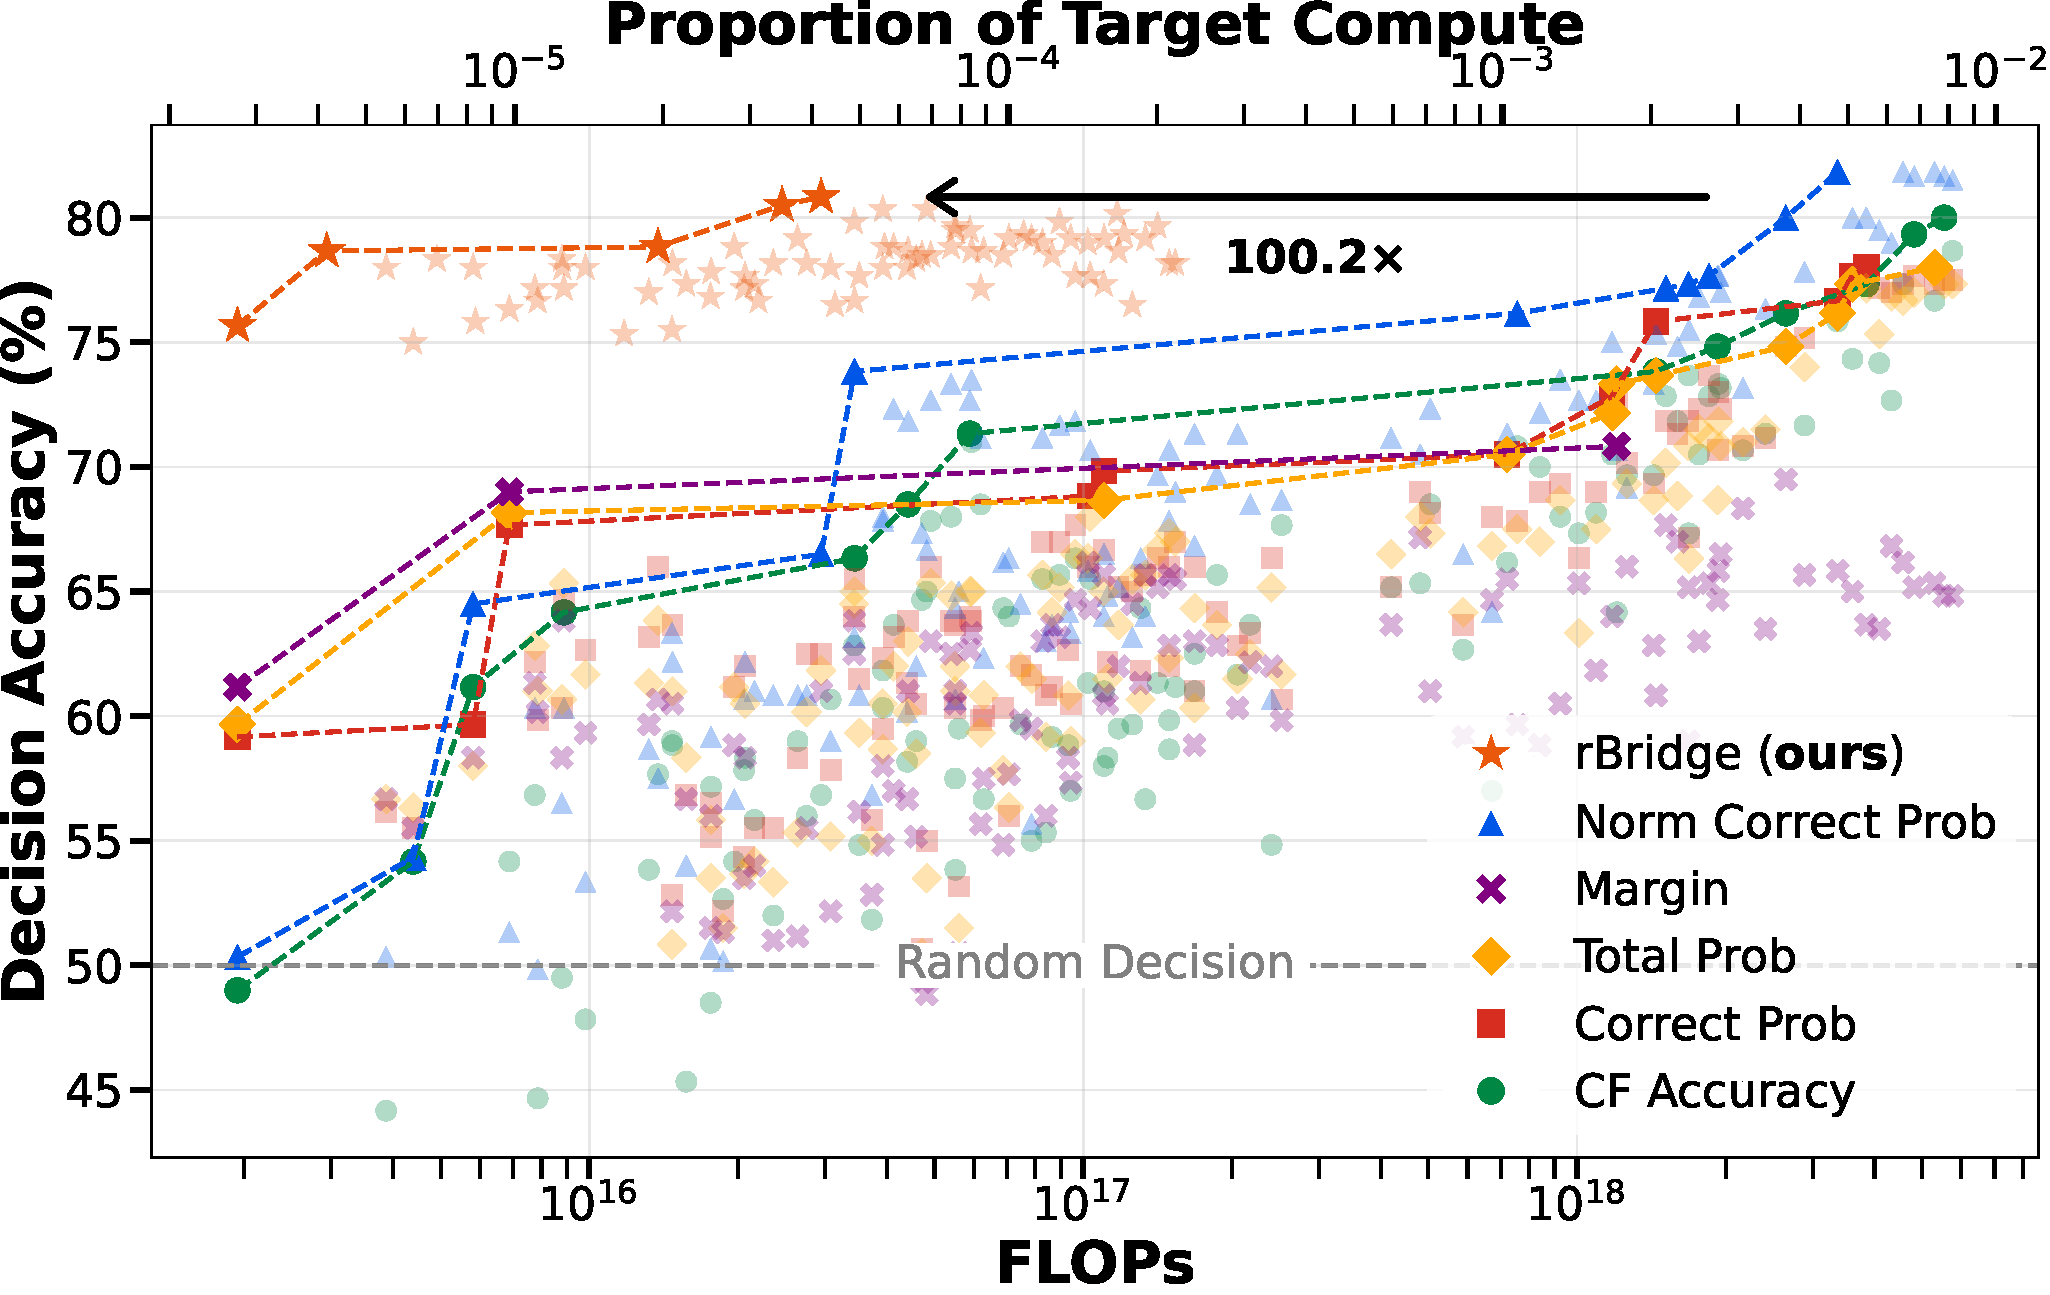
\includegraphics[width=\textwidth]{figs/pareto_decision_accuracy.pdf}
        \caption{Decision Accuracy results across 3.7 - 97.9M proxy model size, and across intermediary checkpoints.}
        \label{fig:pareto}
    \end{subfigure}
    \hfill
    \begin{subfigure}[b]{0.497\textwidth}
        \centering
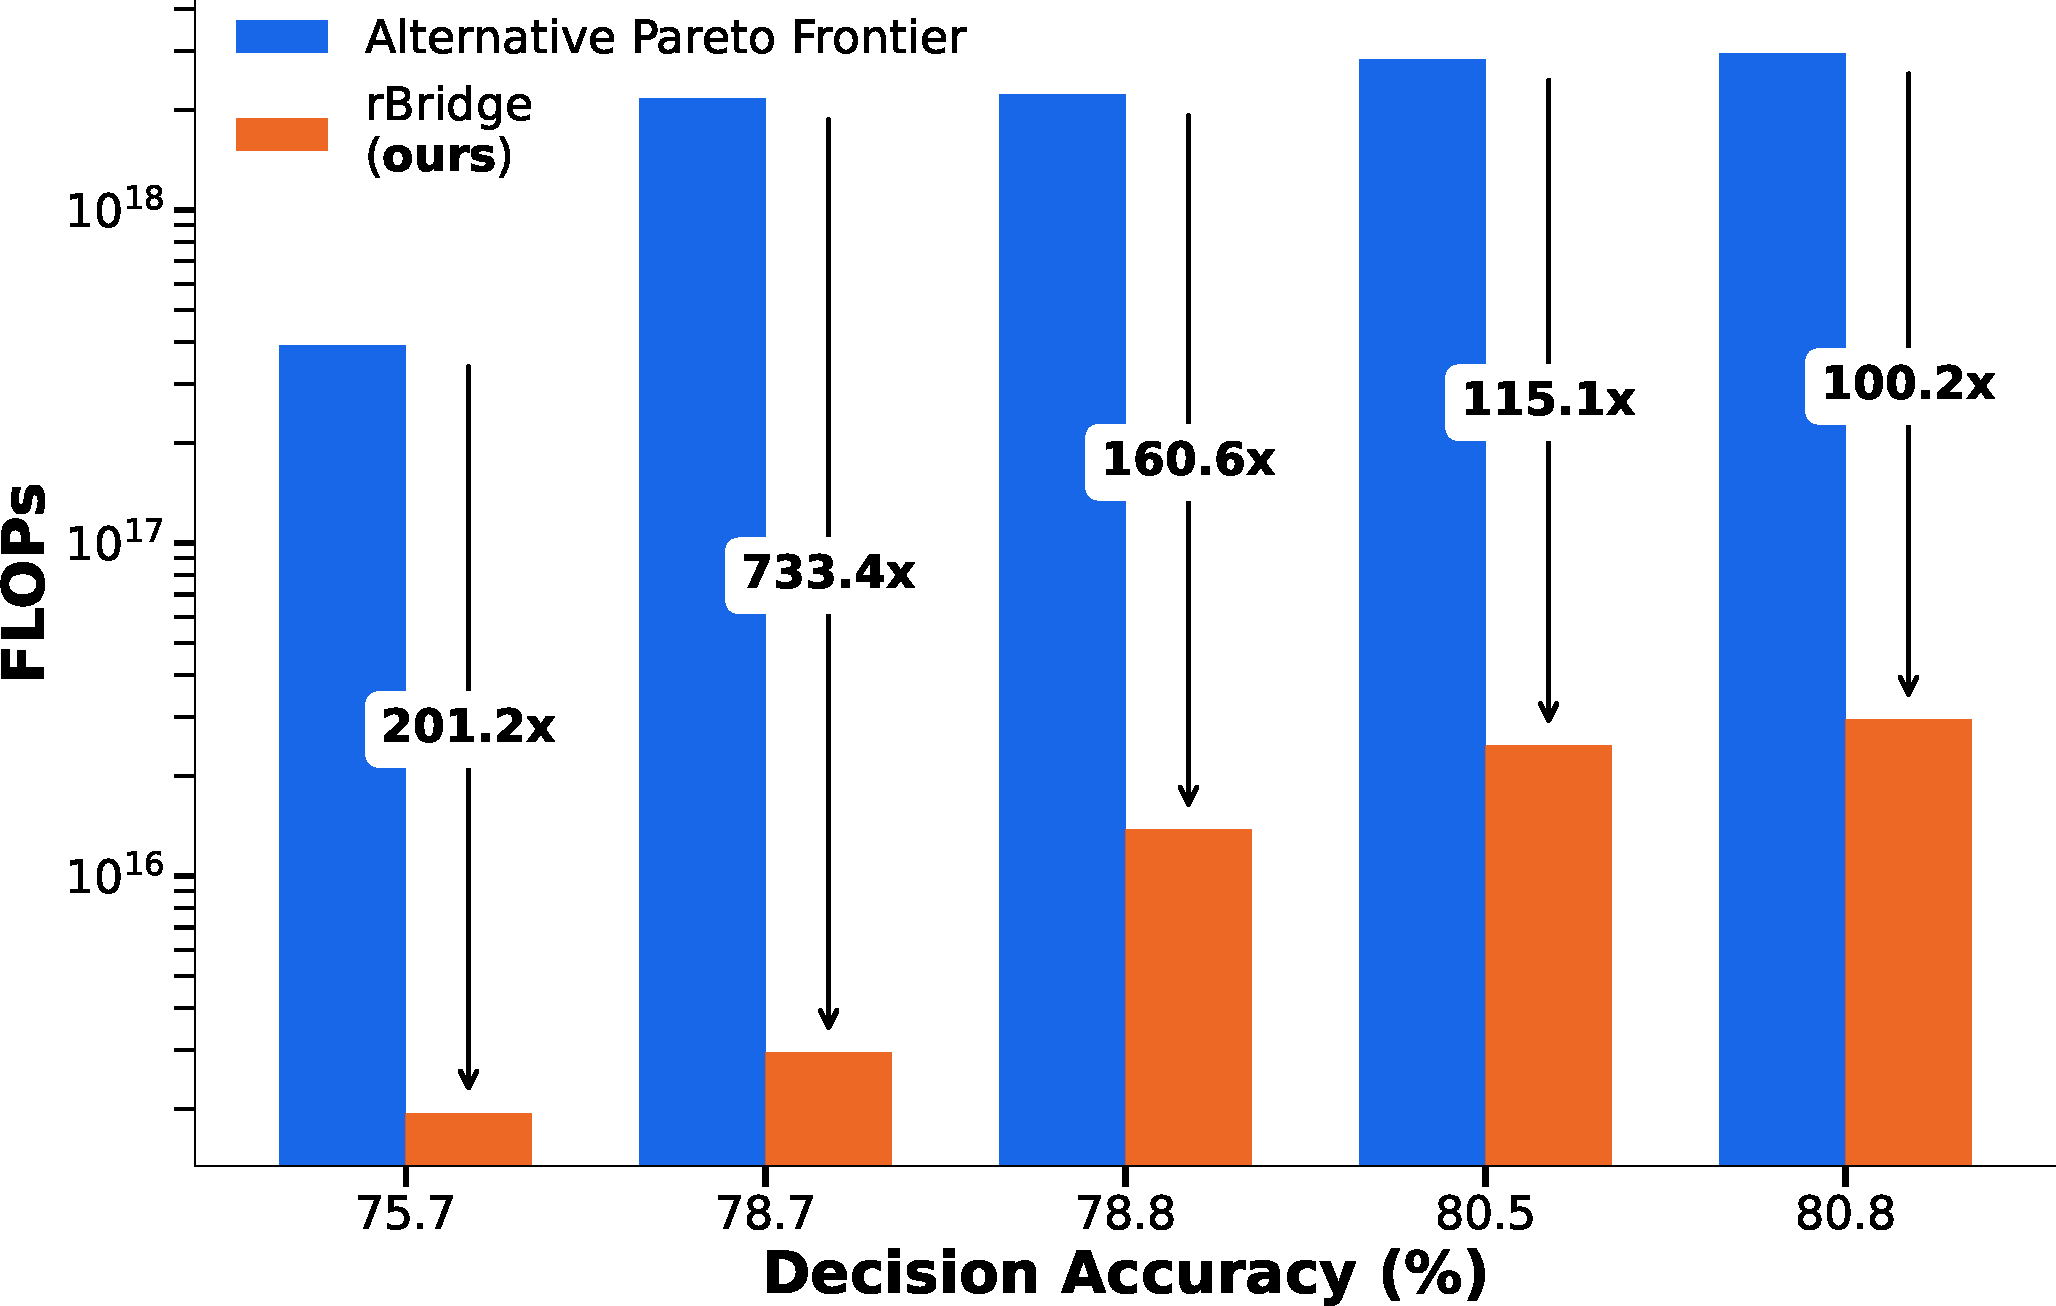
\includegraphics[width=\textwidth]{figs/flops_savings_decision_accuracy.pdf}
        \caption{\tsc{rBridge} saves FLOPs by a factor of 100.2$\times$ to 733.4$\times$.}
        \label{fig:flops}
    \end{subfigure}
    \caption{\tsc{rBridge} improves the pareto frontier in pre-training dataset ranking for 1.2B target model size. Values are averages aggregated across ARC-C and CQA. For intuitive reference, the two most compute efficient points in \tsc{rBridge}'s pareto frontier is (1) 3.7M model size trained on 87.3M tokens, and (2) 6M model size trained on 81.6M tokens.}
    \label{fig:decision_acc}
\end{figure}

\paragraph{Setup.} We curate an additional pre-training dataset $\mc{D}_\text{pre}'$ described in Appendix \ref{app:setting}. Then, we examine how accurate such function as described in \textbf{(ii)}, zero-shot transfers from the OLMo-Mix-1124 to our alternative dataset at 1B $\rightarrow$ 7B at 1T tokens. While larger-scale studies across more model sizes and pre-training datasets would be ideal, training an additional 1B and 7B model for 1T tokens required \textit{thousands} of H100 hours, making further comparisons prohibitively expensive. 

% For instance, at the most compute efficient point representing 3.7M model size trained on 87.3M tokens, \tsc{rBridge} attained DAcc. improvement of +26.7, +25.37, +16.53, +16.03, +14.53, against CF Accuracy, Norm Correct Prob, Correct Prob, Total Prob, and Margin, respectively. This is remarkable as at this proxy compute level, CF Accuracy and Norm Correct Prob displays random decision levels ($\sim$ 50\%). 

% while CF Accuracy and Norm Correct Prob remain near random decision levels ($\sim$50\%). 

% savings FLOPs by a factor of 200.8$\times$ to 920.2$\times$. 

\subsection{Results} \label{sec:result}

\textbf{(i) Over 100$\times$ Dataset Ranking Compute Saving at $<$100M $\rightarrow$ 1.2B.} \tsc{rBridge} significantly improves DAcc. given equivalent compute (Fig. \ref{fig:pareto}). For example, at the most compute-efficient point (3.7M model trained on 87.3M tokens), \tsc{rBridge} achieves up to 27\% higher DAcc. than baseline metrics. This is remarkable as at this proxy compute level, CF Accuracy and Norm Correct Prob displays random decision levels ($\sim$ 50\%). To achieve the same level of DAcc., \tsc{rBridge} uses 100.2$\times$ to 733.4$\times$ less FLOPs (Fig. \ref{fig:flops}).
Kendall’s Tau results are reported in Appendix~\ref{app:more_exp}. As the two evaluation metric are intimately related, the results are highly similar.

\textbf{(ii) Consistently Strongest Relationship at 1B$\rightarrow$13B, 32B.} In 1B $\rightarrow$13B, \tsc{rBridge} achieves the best $R^2$ and MAE in 10/12 cases, and ranks near the top in the remaining two (Tab. \ref{tab:main_tab}). Similar performance occurs in 1B$\rightarrow$13B+SFT where we include a single epoch SFT stage at target scale, and 1B$\rightarrow$32B. For 1B$\rightarrow$13B+SFT and 1B$\rightarrow$32B, granular benchmark-level results appear in Appendix \ref{app:more_exp}.  Aligned with the literature on emergence, discontinuous metrics (Acc./p@1, iSFT) demonstrated worst performance. The remaining continuous metrics performed better, with \tsc{rBridge}'s state-of-the-art performance achieving train $R^2$ of 0.826 - 0.874 and test MAE of 1.304 - 1.481.
\begin{table*}[bt!]
\centering
\resizebox{0.9\textwidth}{!}{%
\begin{tabular}{llcccccc>{\columncolor{gray!15}}c}
\toprule
\textbf{Benchmark} & \textbf{Method:} & \textbf{Acc./p@1} & \textbf{iSFT} & \textbf{TED} & \textbf{MPCA} & \textbf{NLL} & \textbf{R$^\phi$} & \textbf{\tsc{rBridge}} \\
\midrule
\multicolumn{9}{c}{\cellcolor{mybrown!30}\textbf{1B $\rightarrow$ 13B (Pre-to-Pre)}} \\
\midrule
\multirow{2}{*}{GSM8K} & Train R$^2$ & 0.402 & 0.385 & 0.558 & 0.116 & 0.853 & \textbf{0.947} & \underline{0.944} \\
& Test MAE & 5.189 & 4.848 & 5.961 & 84.006 & 3.210 & \underline{1.837} & \textbf{1.751} \\
\midrule
\multirow{2}{*}{MATH500} & Train R$^2$ & 0.127 & 0.076 & 0.213 & 0.025 & 0.861 & \underline{0.864} & \textbf{0.890} \\
& Test MAE & 1.276 & 1.008 & 1.134 & 3.943 & 0.593 & \underline{0.526} & \textbf{0.525} \\
\midrule
\multirow{2}{*}{ARC-C} & Train R$^2$ & 0.200 & 0.166 & 0.547 & 0.319 & 0.166 & \underline{0.950} & \textbf{0.969} \\
& Test MAE & 7.287 & 8.750 & 6.197 & 25.970 & 7.058 & \underline{1.546} & \textbf{1.246} \\
\midrule
\multirow{2}{*}{\makecell{MMLU Pro\\(STEM)}} & Train R$^2$ & 0.167 & --- & 0.199 & 0.200 & \underline{0.207} & \textbf{0.897} & \textbf{0.897} \\
& Test MAE & 1.624 & --- & 1.572 & 1.495 & 12.582 & \underline{0.575} & \textbf{0.574} \\
\midrule
\multirow{2}{*}{CQA} & Train R$^2$ & 0.666 & 0.534 & \underline{0.677} & 0.323 & 0.139 & \textbf{0.890} & \textbf{0.890} \\
& Test MAE & 3.989 & 5.885 & 3.010 & 1697.096 & 5.483 & \underline{2.203} & \textbf{2.182} \\
\midrule
\multirow{2}{*}{HumanEval} & Train R$^2$ & 0.260 & --- & 0.057 & 0.179 & \textbf{0.685} & \underline{0.655} & 0.652 \\
& Test MAE & 2.889 & --- & 2.389 & 3.341 & 2.111 & \underline{2.041} & \textbf{2.025} \\
\midrule
\multicolumn{2}{l}{\textbf{Average Train R$^2$ ($\uparrow$)}} & 0.304 & 0.290 & 0.375 & 0.194 & 0.485 & \underline{0.867} & \textbf{0.874} \\
\multicolumn{2}{l}{\textbf{Average Test MAE ($\downarrow$)}} & 3.709 & 5.123 & 3.377 & 302.642 & 5.173 & \underline{1.455} & \textbf{1.384} \\
\midrule
\multicolumn{9}{c}{\cellcolor{mybrown!30}\textbf{1B $\rightarrow$ 13B + SFT (Pre-to-Post)}} \\
\midrule
\multicolumn{2}{l}{\textbf{Average Train R$^2$ ($\uparrow$)}} & 0.329 & 0.302 & 0.517 & 0.257 & 0.413 & \underline{0.820} & \textbf{0.846} \\
\multicolumn{2}{l}{\textbf{Average Test MAE ($\downarrow$)}} & 4.375 & 5.251 & 4.236 & 27.062 & 3.932 & \underline{1.549} & \textbf{1.304} \\
\midrule
\multicolumn{9}{c}{\cellcolor{mybrown!30}\textbf{1B $\rightarrow$ 32B (Pre-to-Pre)}} \\
\midrule
\multicolumn{2}{l}{\textbf{Average Train R$^2$ ($\uparrow$)}} & 0.312 & 0.349 & 0.352 & 0.205 & 0.488 & \underline{0.820} & \textbf{0.826} \\
\multicolumn{2}{l}{\textbf{Average Test MAE ($\downarrow$)}} & 19.785 & 5.165 & 3.546 & 21.833 & 3.276 & \underline{1.540} & \textbf{1.481} \\
\bottomrule
\end{tabular}
}
\caption{1B$\rightarrow$13B and 1B$\rightarrow$32B performance across mathematics, science, engineering, commonsense, and coding benchmarks. Train fitting and test is done using 5-fold cross validation (\textbf{\S\ \ref{sec:protocol}}). Best value across methods is \textbf{bolded}, and second best is \underline{underlined}.}\label{tab:main_tab}
\end{table*}

% Finally, we ablate the components of \tsc{rBridge} in Fig. \ref{fig:ablation}. Note that we have an ablation study on going from NLL to ScB to R$^\phi$ we propose in \S\ \ref{sec:align}, therefore, skip this part of the ablation study. Here we observe that each part of the \tsc{rBridge} NLL (Eq. \ref{eq:rbridge_nll}) improves performance across all three transfer settings. 

Additionally, even as we increase the proxy model size by 7$\times$, 13$\times$, the target metric fails to out-perform \tsc{rBridge} (Fig. \ref{fig:target_metric}). Notably, \tsc{rBridge}'s and best alternative box-and-whisker's box does not overlap, suggesting a meaningful improvement. To understand where these gains originate, we ablate the components of \tsc{rBridge} in Fig.~\ref{fig:ablation}, showing that each part of the \tsc{rBridge} NLL (Eq.~\ref{eq:rbridge_nll}) plays an important role to its effectiveness across all three experimental settings. Note that we have an ablation study on going from NLL to ScB to R$^\phi$ in \textbf{\S\ \ref{sec:align}}, therefore, skip this part here.

% Similarly, the MinMax normalization stage consistently improves predictive performance as seen by the decrease in MAE, albeit with a lower magnitude of improvement. While the degree of improvement with MinMax normalization may not be large, this provides further evidence that the weighting scheme in Eq. \ref{eq:rbridge_nll} is salient, as the normalization stage amplifies the weight factor's effective where lower weights are given even lower weights, and vice-versa.

\paragraph{(iii) Successful Zero-shot Functional Relationship Transfer at 1B$\rightarrow$7B.} We demonstrate that functions fitted on dataset $\mc{D}_\text{pre}$ with \tsc{rBridge} (from \textbf{(ii)}) can zero-shot transfer to alternative pre-training dataset $\mc{D}_\text{pre}'$, reducing additional experimental compute cost by factor $\frac{m}{n}$ (Tab. \ref{tab:function}). In our experiment setting of 1B$\rightarrow$7B, this yields a 7$\times$ compute reduction since only a proxy model of $\frac{1}{7}$ the target size is required. The transferred function achieves low MAE of 0.043 - 1.417 across most benchmarks (one outlier at 9.716), outperforming $R^\phi$. For dataset ranking using predicted accuracy, \tsc{rBridge} achieves perfect 5/5 performance versus $R^\phi$'s 4/5. This demonstrates that improved function fitting from \textbf{(ii)} translates to superior zero-shot transfer performance across datasets.
\begin{figure}[tb]
    \centering
    \begin{subfigure}[b]{0.497\textwidth}
        \centering
        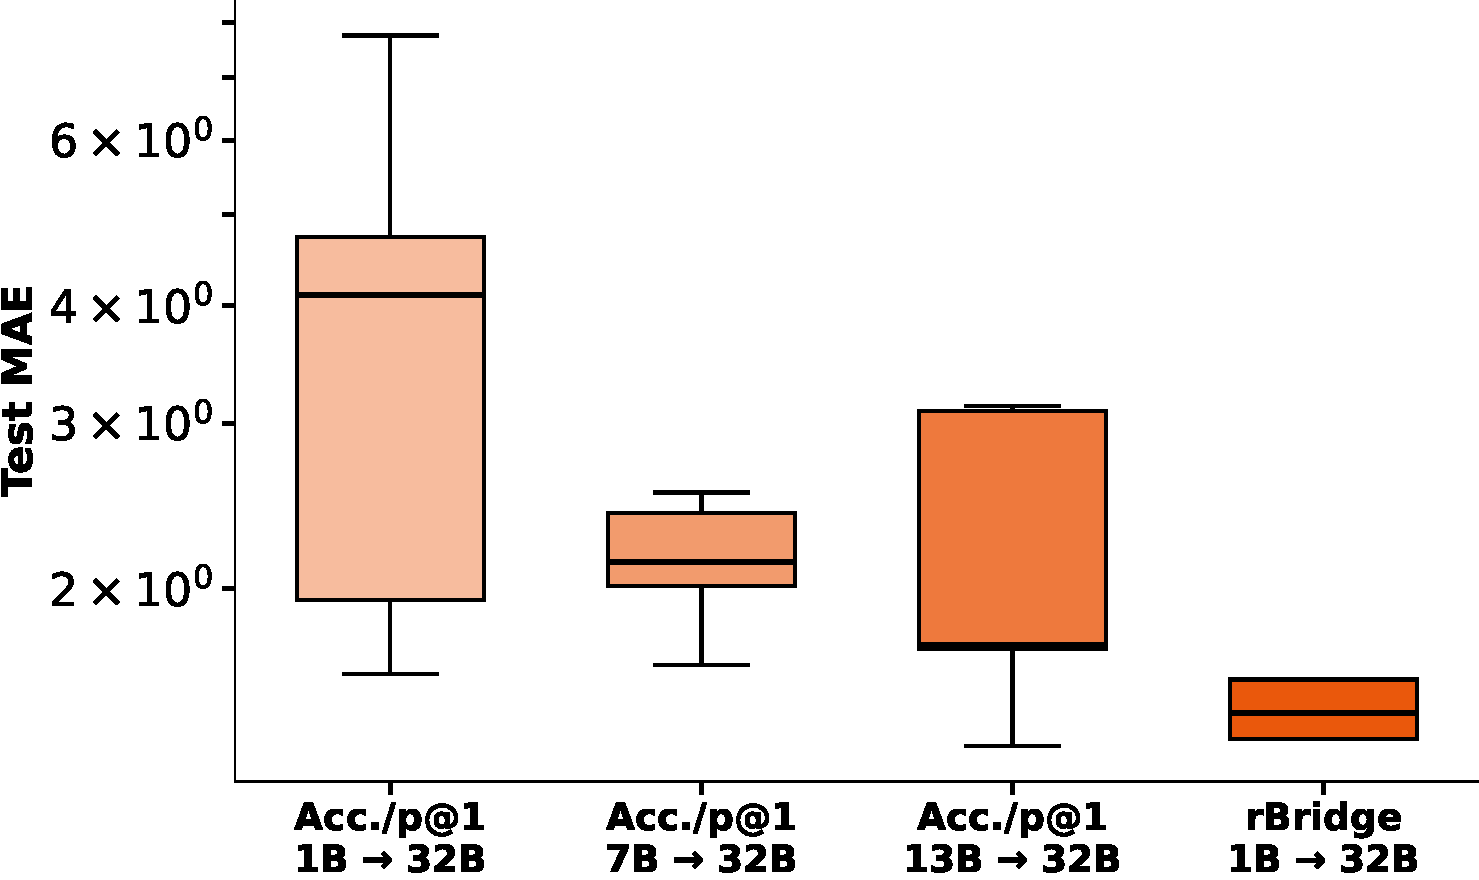
\includegraphics[width=\textwidth]{figs/downstream.pdf}
        \caption{\tsc{rBridge} outperforms proxy models 7 - 13$\times$ larger using the target metric (Acc./p@1).}
        \label{fig:target_metric}
    \end{subfigure}
    \hfill
    \begin{subfigure}[b]{0.497\textwidth}
        \centering
        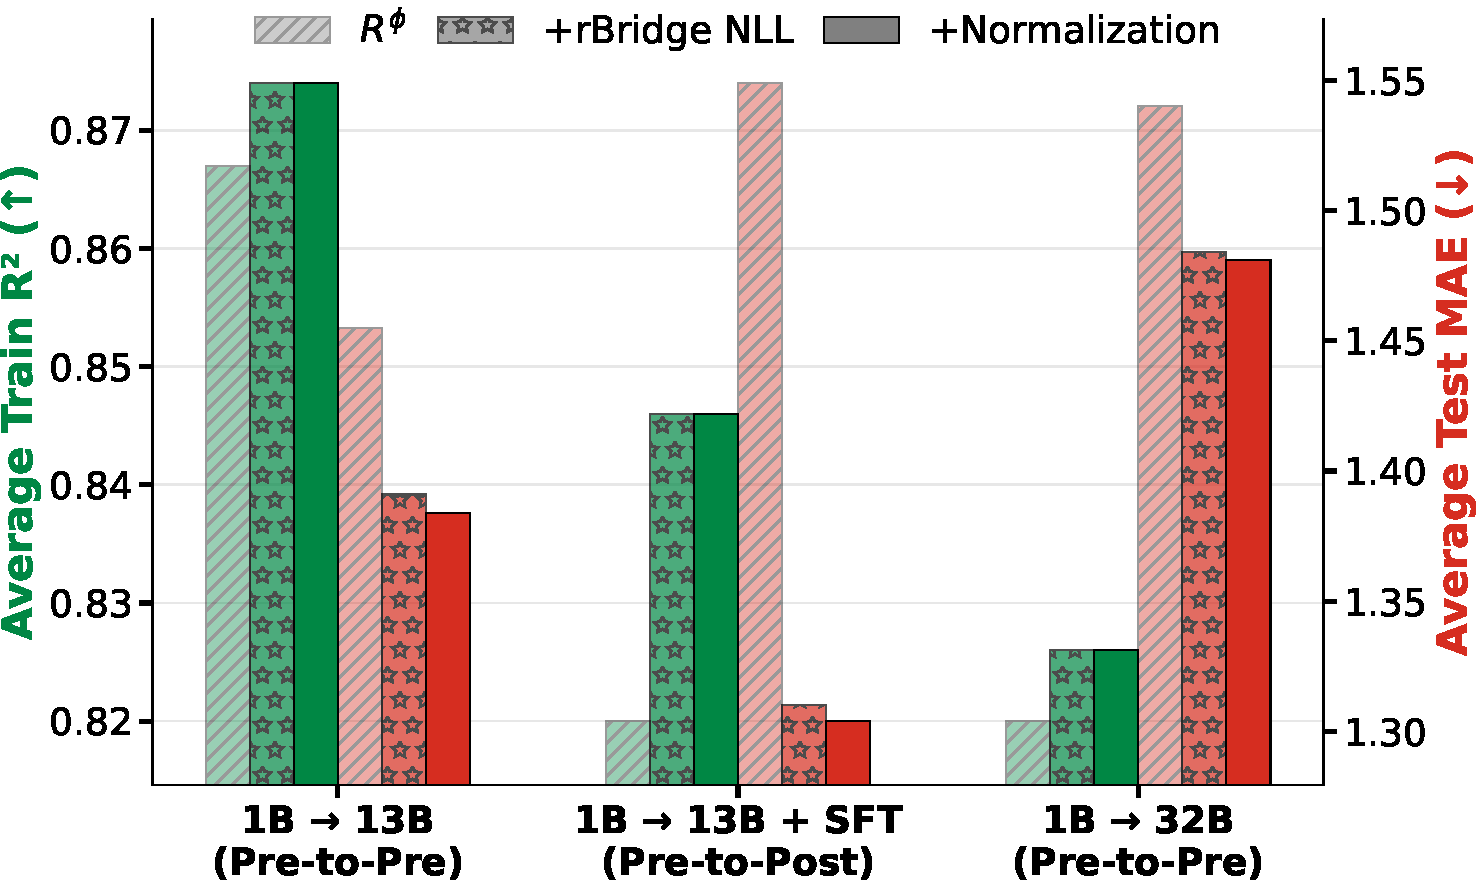
\includegraphics[width=\textwidth]{figs/ablation.pdf}
        \caption{Ablation shows that \tsc{rBridge} NLL and normalization results in consistent improvement.}
        \label{fig:ablation}
    \end{subfigure}
    \caption{Additional experimental results demonstrate clear advantages of our proposed method.}
    \label{fig:additional}
\end{figure}


\begin{table*}[tb]
\centering
\resizebox{\textwidth}{!}{
\begin{tabular}{l|l|ccccc|c}
\toprule
\multicolumn{8}{c}{\cellcolor{mybrown!30}\textbf{1B $\rightarrow$ 7B Zero-shot Functional Relationship Transfer from $\mc{D}_\text{pre}$ to $\mc{D}'_\text{pre}$}} \\
\midrule
\textbf{Method} & \textbf{Benchmark:} & \textbf{GSM8K} & \textbf{MATH500} & \textbf{ARC-C} & \textbf{MMLU Pro} & \textbf{CQA} & \textbf{Average} \\
\midrule
\multirow{2}{*}{\textbf{Ground Truth}} & \textbf{Acc. (\%) of $\mc{D}_\text{pre}$} & \cellcolor{mygreen!30}10.538 & \cellcolor{myred!30}2.800 & \cellcolor{mygreen!30}56.911 & \cellcolor{mygreen!30}10.225 & \cellcolor{mygreen!30}60.442 & 28.183\\
 & \textbf{Acc. (\%) of $\mc{D}_\text{pre}'$} & \cellcolor{myred!30}8.264 & \cellcolor{mygreen!30}3.600 & \cellcolor{myred!30}51.536& \cellcolor{myred!30}9.578 & \cellcolor{myred!30}44.554 & 23.506 \\
 \midrule
\multirow{3}{*}{\textbf{R$^\phi$}} & \textbf{Acc. (\%) Prediction of $\mc{D}_\text{pre}'$} & 9.886 & 3.116 & 52.558 & 10.649 & 57.479 & 26.738 \\
 & \cellcolor{gray!30}\textbf{Rank($\mc{D}_\text{pre}$, $\mc{D}_\text{pre}'$) w. Prediction ($\uparrow$)} & \cellcolor{gray!30}\textcolor{mygreen}{\checkmark} & \cellcolor{gray!30}\textcolor{mygreen}{\checkmark}& \cellcolor{gray!30}\textcolor{mygreen}{\checkmark} & \cellcolor{gray!30}\textcolor{myred}{\texttimes} & \cellcolor{gray!30}\textcolor{mygreen}{\checkmark} & \cellcolor{gray!30}4/5 \\
 & \cellcolor{gray!30}\textbf{MAE ($\downarrow$)} & \cellcolor{gray!30}1.622 & \cellcolor{gray!30}0.484 & \cellcolor{gray!30}1.022 & \cellcolor{gray!30}1.071 & \cellcolor{gray!30}12.926 & \cellcolor{gray!30}3.425 \\
  \midrule
\multirow{3}{*}{\textbf{rBridge}} & \textbf{Acc. (\%) Prediction of $\mc{D}_\text{pre}'$} & 8.220 & 3.044 & 52.254 & 8.161 & 54.269 & 25.190 \\
 & \cellcolor{gray!30}\textbf{Rank($\mc{D}_\text{pre}$, $\mc{D}_\text{pre}'$) w. Prediction ($\uparrow$)} & \cellcolor{gray!30} \textcolor{mygreen}{\checkmark} & \cellcolor{gray!30} \textcolor{mygreen}{\checkmark}& \cellcolor{gray!30}\textcolor{mygreen}{\checkmark} & \cellcolor{gray!30}\textcolor{mygreen}{\checkmark} & \cellcolor{gray!30}\textcolor{mygreen}{\checkmark} & \cellcolor{gray!30} \textbf{5/5} \\
 & \cellcolor{gray!30}\textbf{MAE ($\downarrow$)} & \cellcolor{gray!30} 0.043 & \cellcolor{gray!30}0.556 & \cellcolor{gray!30}0.718 & \cellcolor{gray!30}1.417 & \cellcolor{gray!30}9.716 & \cellcolor{gray!30} \textbf{2.490} \\
\bottomrule
\end{tabular}
}
\caption{\tsc{rBridge} demonstrates strong zero-shot functional relationship transfer across datasets. Ground Truth rows are the Acc. performance and ranking ({\setlength{\fboxsep}{2pt}\colorbox{mygreen!30}{rank 1}, \colorbox{myred!30}{rank 2}}) that the prediction is aiming to attain. \tsc{rBridge} achieves 0 - 1.5 (\%) error-rate excluding one outlier, and perfectly ranks the datasets on all five benchmarks. Average values are aggregated across the row. }\label{tab:function}
\end{table*}

% \paragraph{[1] Intra-dataset $\Delta$.} For intra-dataset $\Delta$ we employ $5$-fold cross validation following \cite{che2018recurrent}, \cite{lee2020biobert}. Across 5-folds, we report the average curve fitting relationship R$^2$ on the train set and test Mean Absolute Error (MAE; \cite{chai2014root}). The proxy to target model scale we examine is 1B $\rightarrow$ 13B, 32B, with pre-trained tokens ranging 250 - 3750B tokens with evaluations in intervals of 250B tokens. We also include a Pre-to-Post study which examines how well the proxy model can predict pre-trained models with an additional SFT stage. The pre-training dataset is OLMo-Mix-1124 \citep{olmo20242}. We select six representative reasoning benchmarks spanning mathematics, science, engineering, commonsense, and coding: GSM8K, MATH500, ARC-C \citep{clark2018think}, MMLU Pro \citep{wang2024mmlupro} (STEM subset), CQA \citep{talmor-etal-2019-commonsenseqa}, and HumanEval \citep{chen2021evaluating}.

% \paragraph{[1] Baselines.} We cover 6 alternative metrics that examine the relationship of small and large models given the same data source, and metrics that have shown non-emergent continuity at small scale. First, we include the most naïve approach, the target metric: Accuracy and Pass@1 (Acc./p@1; \cite{NEURIPS2019_7298332f}). Second, we include intermediate supervised fine-tuning (iSFT; \cite{snell2024predicting}) which demonstrate that including a SFT stage throughout the intermediate pre-training checkpoints help target metric (Acc./p@1) be used as signals in smaller models with less training compute. Third is Token Edit Distance (TED; \cite{NEURIPS2023_adc98a26}) which showed that emergence occurs due to discontinuous metrics. Fourth is Model Probability of Correct Answer (MPCA) as demonstrated in \cite{NEURIPS2023_adc98a26}, \cite{snell2024predicting} as a continuous metric. Last is ScB which visualize the relationship between ScB and target metric using multi-scale smaller models. As mentioned in \S\ \ref{sec:target_align}, we use our proposed improved version of ScB, R$^\phi$, as there were insufficient details to replicate ScB on all of our benchmarks.

% A final challenge in using ScB as a baseline is the lack of instructions to replicate their method for benchmarks' $Y^*$ that they have not released. For instance, while we want to evaluate on GSM8K, we do not have a followable format for generating the $Y^*$ as their HuggingFace dataset indicate a \textit{unique} instruction format for each benchmark. 

\section{Discussion}\label{sec:discussion}

\paragraph{Additional Related Work.} \cite{zhang2024predictable} uses proxy benchmarks with small proxy models to predict pre-training performance of larger target models. However, their approach suffers from several limitations. First, it is computationally expensive, requiring global search over 42 benchmarks and 34 models. Second, the required size of the search space (number of benchmarks and models) lacks principled justification. Third, using fundamentally different test distributions introduces suboptimal noise, as we empirically demonstrate in Appendix \ref{app:proxy_task}. 

\cite{xie2023doremi} and \cite{liu2025regmix} leverage small proxy models (1 to 280M parameters) to optimize pre-training data \textit{mixture weights} for larger target models ($\sim$7B), operating under the assumption that small-scale performance meaningfully correlates with large-scale performance. Both works rely on standard NLL or perplexity metrics, which we demonstrate to be suboptimal in \textbf{\S\ \ref{sec:limit}}. Furthermore, their experiments are predominantly on non-emergent benchmarks (e.g., TriviaQA and HellaSwag), whereas our work specifically targets reasoning benchmarks that exhibit emergent behavior. Lastly, their approaches are specialized for optimizing pre-training data \textit{mixtures}, whereas our method addresses the more general problem of predicting large model performance with small proxy models, enabling \textit{broader} applications.

Moreover, readers can view \cite{10651521}, \cite{10.1145/3706118}, \cite{kipnis2025metabench}, and \cite{pacchiardi-etal-2025-predictaboard} for some past works on LLM performance prediction, and evaluation. We acknowledge that alternative branches of the literature have studied predicting LLM performance.

\paragraph{Minimal Compute Overhead.} While \tsc{rBridge} introduces some additional costs, these are minor. First, is generating the gold reasoning trace $R^\phi$ via the frontier model. However, this represents a small one-time cost of under \$10 per benchmark. To help the research community we plan to open-sourced our dataset, allowing future researchers to skip this cost for benchmarks we examine. Second, the automatic weighting mechanism (Fig. \ref{fig:rbridge}) incurs only a few seconds of CPU runtime per benchmark. Both overheads are negligible compared to the computational savings our method provides.
% \paragraph{Technical Takeaway: Pre-training Evaluation Objective and Task Alignment.} Our main technical finding is that we should attempt to find an output $Y^*$ that is more ID while ensuring that it is task aligned. We first demonstrate that we can increase level of ID by using a frontier model's reasoning trace $R^\phi$ as $Y^*$ (\S\ \ref{sec:easy}, Fig. \ref{fig:idood}). Our empirical finding here is that we should minimize any formatting that is unnatural to the pre-training distribution, e.g., "Final Answer: $\cdots$". Furthermore, $R^\phi$ is well aligned with the task, as it is the intermediary process that leads to the downstream final answer (Fig. \ref{fig:scb_clean}, Tab. \ref{tab:scb}). Then, we further improve task alignment by automatically weighting each token by its level of task alignment during NLL evaluation (\S\ \ref{sec:target_align}, Fig. \ref{fig:diagram}). 

\paragraph{\tsc{rBridge} is a Better Predictor of Large Scale Pre-training Performance on Reasoning.} While we would expect the \textit{same} metric to yield the greatest relationship and predictive power, our paper demonstrates that this is not the case. As visualized in Fig. \ref{fig:target_metric} even as we scale the proxy model by 7$\times$, 13$\times$, it fails to achieve the performance levels of \tsc{rBridge}. Our work empirically demonstrates that improved alignment with the \textbf{(1)} pre-training evaluation objective, and the \textbf{(2)} task is key to successfully leveraging small models to proxy large model's reasoning performance. Our ablative studies clearly indicate that each component \textbf{(1, 2)} of \tsc{rBridge} is valuable 
(Tab. \ref{tab:scb}, Fig. \ref{fig:ablation}).


\paragraph{Significant Compute and Economic Cost Reduction.} We observe definitive computational cost saving gains through \tsc{rBridge}. In our first experiment \textbf{(i)}, we demonstrate that through \tsc{rBridge} proxy models that are 324.3$\times$ (proxy models $\frac{3.7}{1200}$ the size of target) smaller can be strong proxies for dataset ranking. From a computational perspective, \tsc{rBridge} achieve at least 100.2$\times$ compute savings against the best baseline in achieving the same ranking performance. In our second experiment \textbf{(ii)}, we demonstrate that 13$\times$ and 32$\times$ smaller proxy models can be effectively used as proxies. We believe that \tsc{rBridge}'s utility extrapolates to much greater proxy-target model scale differences. It is also important to note that, by extension, \tsc{rBridge} has the potential to significantly reduce environmental footprint. This has meaningful societal impact as foundation model development has consequential environmental costs \citep{winsta2025hidden,morrison2025holistically}.

% First, \tsc{rBridge} is shown to be state-of-the-art and most reliable across numerous benchmarks and 3$\times$ transfer settings (Tab. \ref{tab:main_tab}, Fig. \ref{fig:target_metric}). Additionally, dramatically improves the pre-training compute needed to search for optimal datasets (Fig. \ref{fig:pareto}, \ref{fig:flops}). 

\paragraph{Enabling Zero-shot Functional Relationship Transfer Across Datasets.} To our knowledge, we are the first to show that the proxy-target function fitted on one pre-training dataset (as shown in experiment \textbf{(ii)}) can be successfully transferred to an alternative one, with no additional fitting. We observe that the improved relationship fitting of \tsc{rBridge} in experiment \textbf{(ii)}'s Tab. \ref{tab:main_tab} extends to improved prediction (MAE) and ranking performance in Tab. \ref{tab:function}. This saves $\frac{m}{n}\times$ compute as any additional pre-training dataset's performance can be reasonably approximated.

\paragraph{Practical Potential Application: Two-stage Dataset Optimization.} 

Practitioners optimizing pre-training data navigate a vast candidate space of data sources and mixtures \citep{xie2023doremi, han2025trillion, liu2025regmix}. The experiments in \textbf{\S\ \ref{sec:exp}} provide a practically applicable framework for such dataset optimization that can be derived as a strong future work. \textbf{[Stage 1]} Given $N$ candidate datasets, following the setting of experiment \textbf{(i)} offers a cost-effective way to filter out $N - k$ poor datasets at e.g. $<$100M proxy scale, reducing the candidate space to $k$. With high decision accuracy of $\sim$80\% (Fig. \ref{fig:decision_acc}), we can expect bad datasets to have been filtered out correctly. Using relatively easier reasoning benchmarks (e.g., ARC-C) suffices for filtering out \textit{weak} datasets. This approach works because (1) strong candidates must also perform well on these tasks, and (2) their performance still correlates with more difficult ones (Fig. \ref{fig:proxytask}), even if they are not strong enough to serve as accurate predictors for ranking the downstream reasoning task. \textbf{[Stage 2]} For the remaining $k$ datasets, we train larger 1B-scale proxies following \textbf{(ii)} and \textbf{(iii)} to accurately rank them by predicting performance at the target scale (e.g., 32B). Although one training run at the target scale $m$ is needed, it is rare for practitioners to work without a baseline target model to improve upon. 

Denoting the required proxy and target compute as $C^\text{p}_1$ and $C^\text{p}_2$ for proxies and $C^\text{t}$ for target, it can be assumed that these costs $C$ are directly proportional to model size \citep{kaplan2020scaling}. The required total compute under this framework is $NC^\text{p}_1 + kC^\text{p}_2 + C^\text{t}$ compared to the naïve approach cost $NC^\text{t}$. Given that the cost reduction factor is $\frac{NC^\text{t}}{NC^\text{p}_1 + kC^\text{p}_2 + C^\text{t}}$, and $C^\text{p}_1, C^\text{p}_2 \ll C^\text{t}$, we can see how cost savings improve as the number of candidate datasets $N$ enlarge. Considering that the candidate space $N$ is very large in the real-world, this framework enables practitioners to optimize pre-training datasets at a fraction of the cost.

% \paragraph{Limitation and Future Direction.} We discuss limitation and more future direction in Appendix. \ref{app:limitation}.
\subsection{Limitation and Future Direction} \label{app:limitation}

We discuss several limitations of \textsc{rBridge} that present opportunities for future research. First, frontier models do not achieve perfect accuracy on reasoning tasks, potentially resulting in imperfect extracted reasoning trace $R^\phi$. While we utilize all available $R^\phi$ without filtering and demonstrate substantial performance and efficiency gains. Our preliminary experiments showed minimal improvements from post-hoc filtering of incorrect generations. Future work could investigate more sophisticated quality assurance mechanisms, such as ensemble methods leveraging multiple frontier models.

Second, frontier models occasionally fail to produce outputs in the required format for reasoning trace $R^\phi$ extraction. Our current approach provides one additional generation attempt before excluding the sample from training. This represents a limitation that future research could address through more robust prompt engineering, or ensembling multiple frontier models.

Finally, while we present a potential framework for further practical application in \textbf{\S\ \ref{sec:discussion}}, the efficient and effective implementation of this system remains an open challenge. Future work can further explore how to best leverage the methodological contribution of \tsc{rBridge} (\textbf{\S\ \ref{sec:rbridge}}) and experimental robustness (\textbf{\S\ \ref{sec:exp}}) on more complex frameworks.

% From this, they can derive the predictive functional form between \tsc{rBridge} and the target metrics. 

% While the value of $k$ can be chosen by considering the compute budget required to achieve the desired accuracy, assuming $k=10$, $N=100$, $m=$ 7B with equivalent trained tokens across model sizes, and the mentioned proxy size $n=$ 0.09B results in $\sim$4\% of the cost incurred by the naïve approach of optimizing at target scale. 


\newpage
\section{Ethics Statement} \label{app:ethic}
Our work conforms to the ICLR Code of Ethics. We report minor use of LLMs for polishing writing. All LLM-generated content has been reviewed and verified by the authors, who take full responsibility for the accuracy and integrity of the work presented.

\section{Reproducibility Statement} \label{app:reproduce}
Our method \tsc{rBridge} is fully reproducible using the information provided in this paper. The approach follows a straightforward process: applying a specific prompt to a frontier model, then computing our proposed negative log-likelihood as presented in Eq. (\ref{eq:rbridge_nll}) and illustrated in Fig. \ref{fig:rbridge}. We provide the exact prompt in  Appendix \ref{app:pseudocode} along with pseudocode (Alg. \ref{alg:rbridge}) for implementation. To further support reproducibility and benefit the research community, we open-sourced our dataset.

\section{Acknowledgment} 
This research was fully funded by Trillion Labs. Se-Young Yun was partially supported by the Institute of Information \& communications Technology Planning \& Evaluation (IITP) grant funded by the Korea government (MSIT) (No. 2022-0-00871, Development of AI Autonomy and Knowledge Enhancement for AI Agent Collaboration).

\bibliography{iclr2025_conference}
\bibliographystyle{iclr2025_conference}

\newpage
\appendix
\section*{\textbf{Appendix}}

\section{Additional results on noisy small scale models} \label{app:noisy}

Refer to Fig. \ref{fig:motivation_app}.

\begin{figure}[htb]
    \centering

    \begin{subfigure}[b]{0.497\textwidth}
        \centering
        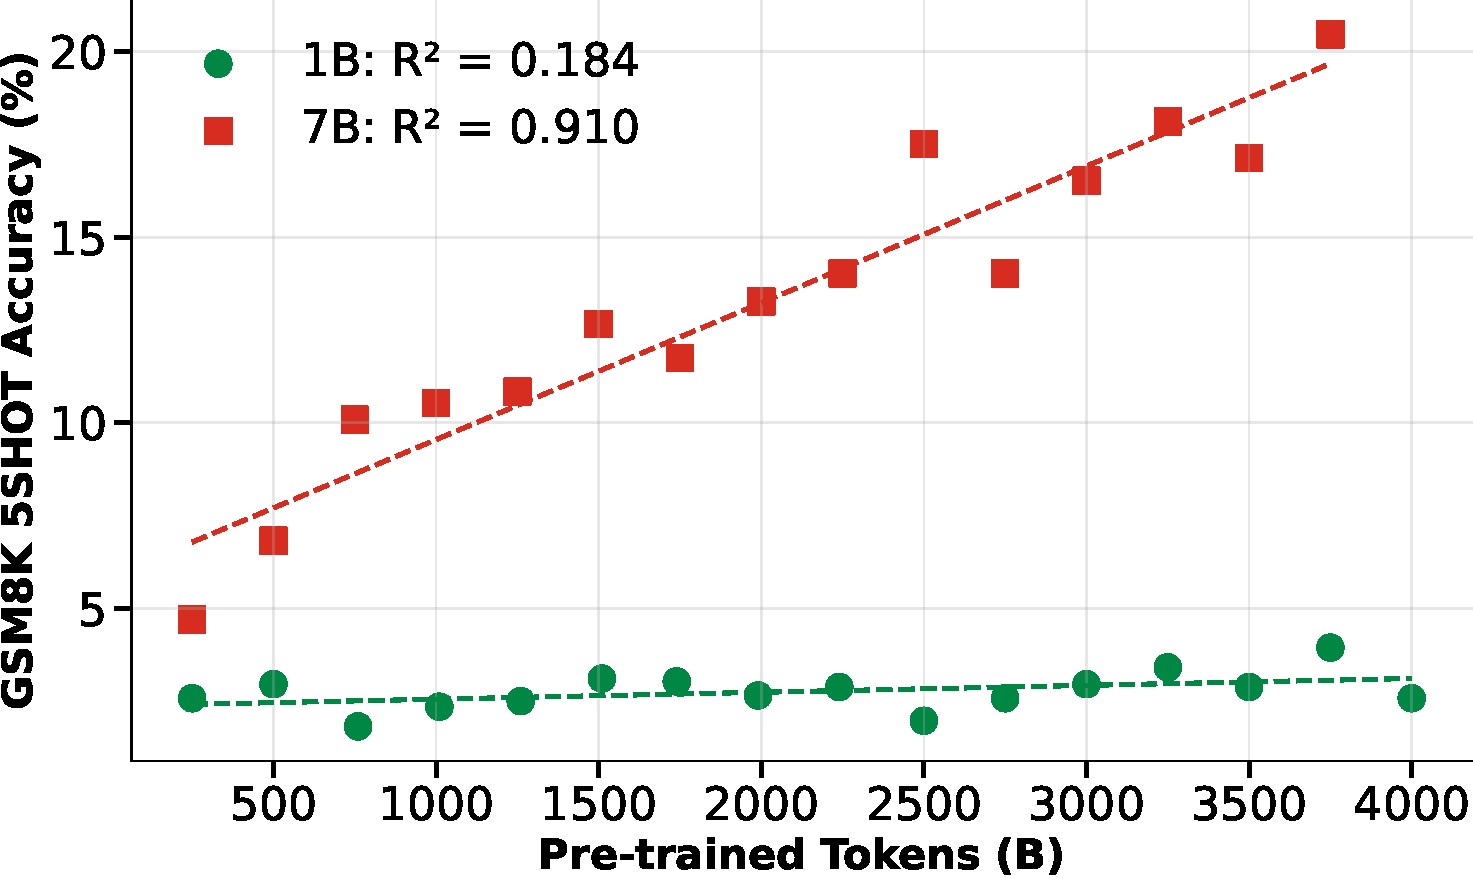
\includegraphics[width=\textwidth]{figs/gsm8k_5shot_1b_7b_performance.pdf}
    \end{subfigure}
    \hfill
    \begin{subfigure}[b]{0.497\textwidth}
        \centering
        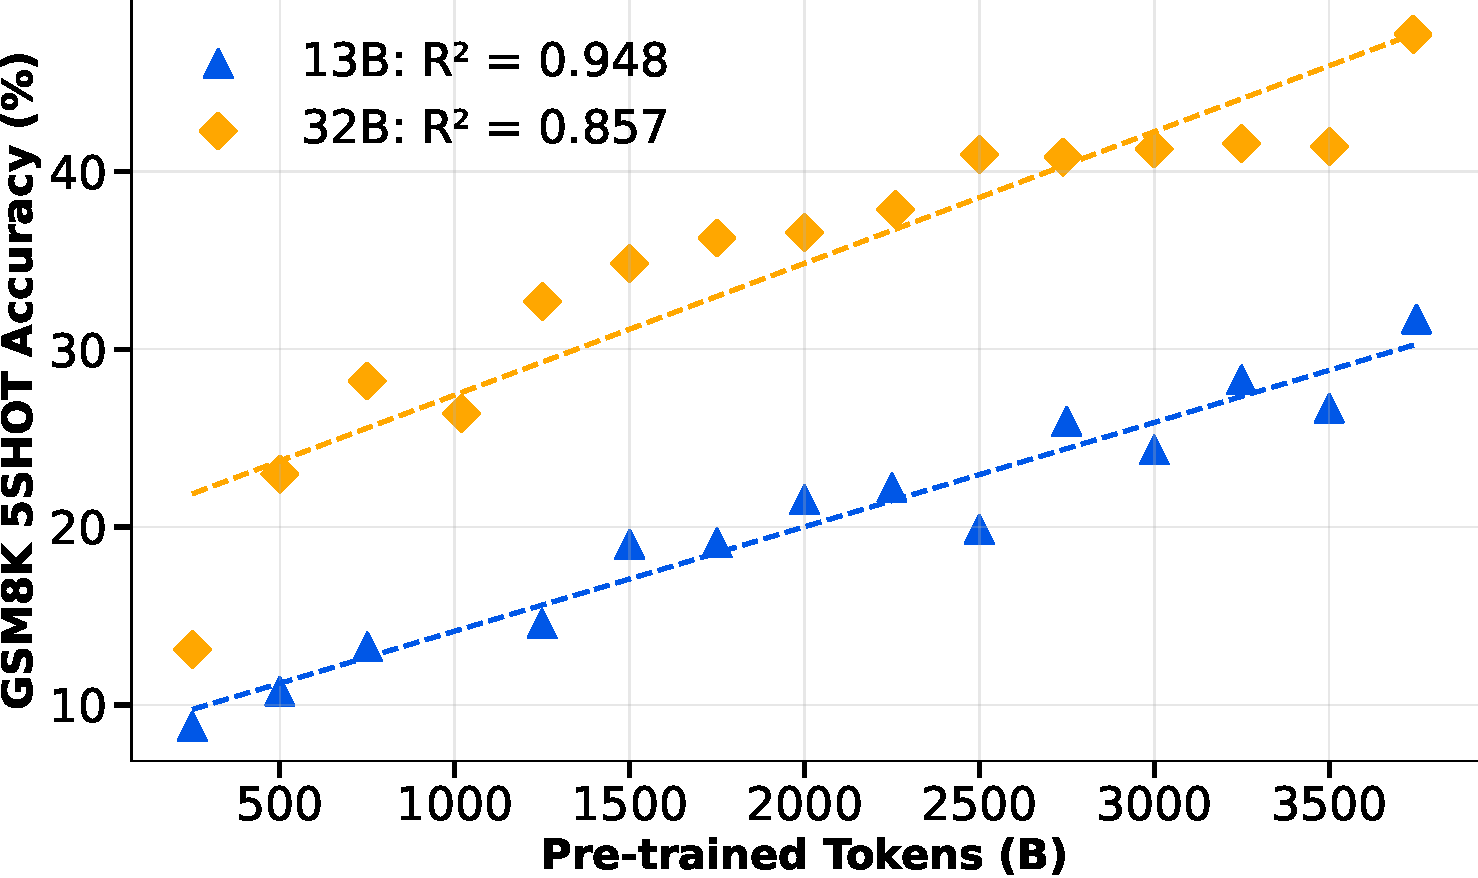
\includegraphics[width=\textwidth]{figs/gsm8k_5shot_13b_32b_performance.pdf}
    \end{subfigure}

    \begin{subfigure}[b]{0.497\textwidth}
        \centering
        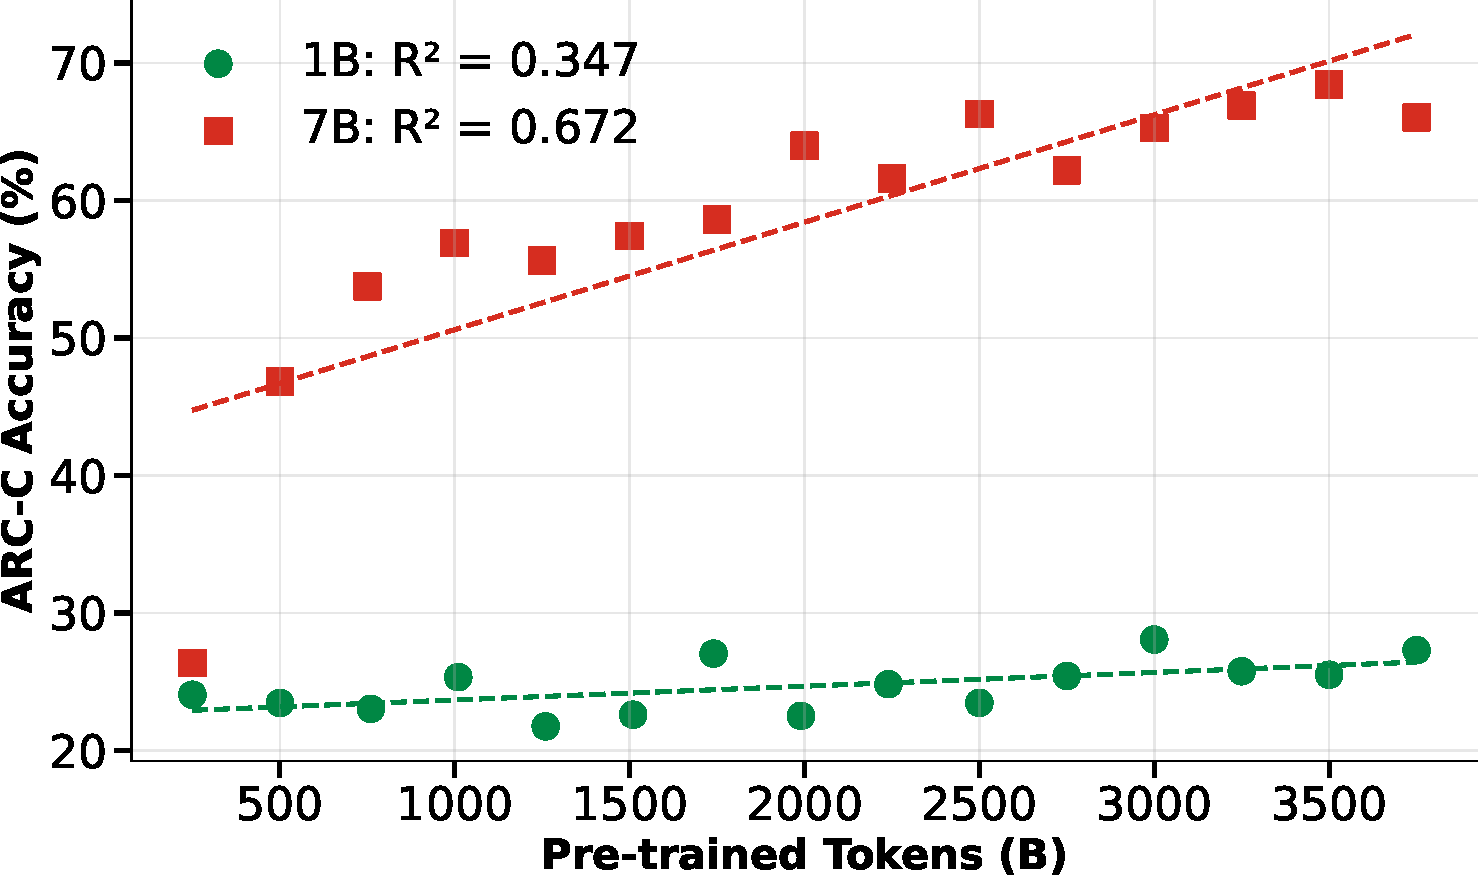
\includegraphics[width=\textwidth]{figs/arc-c_1b_7b_performance.pdf}
    \end{subfigure}
    \hfill
    \begin{subfigure}[b]{0.497\textwidth}
        \centering
        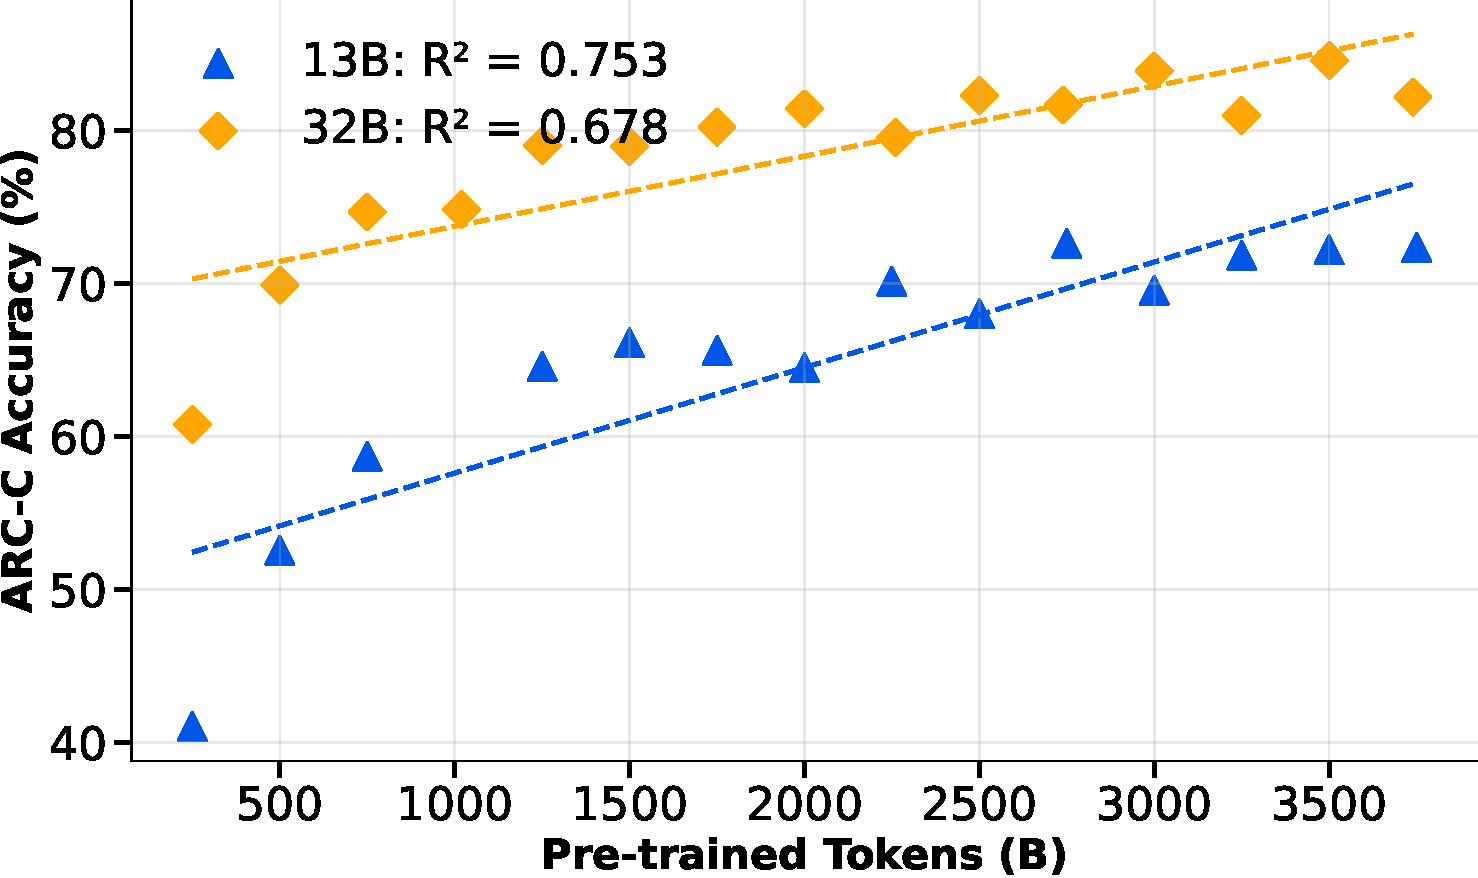
\includegraphics[width=\textwidth]{figs/arc-c_13b_32b_performance.pdf}
    \end{subfigure}

    \begin{subfigure}[b]{0.497\textwidth}
        \centering
        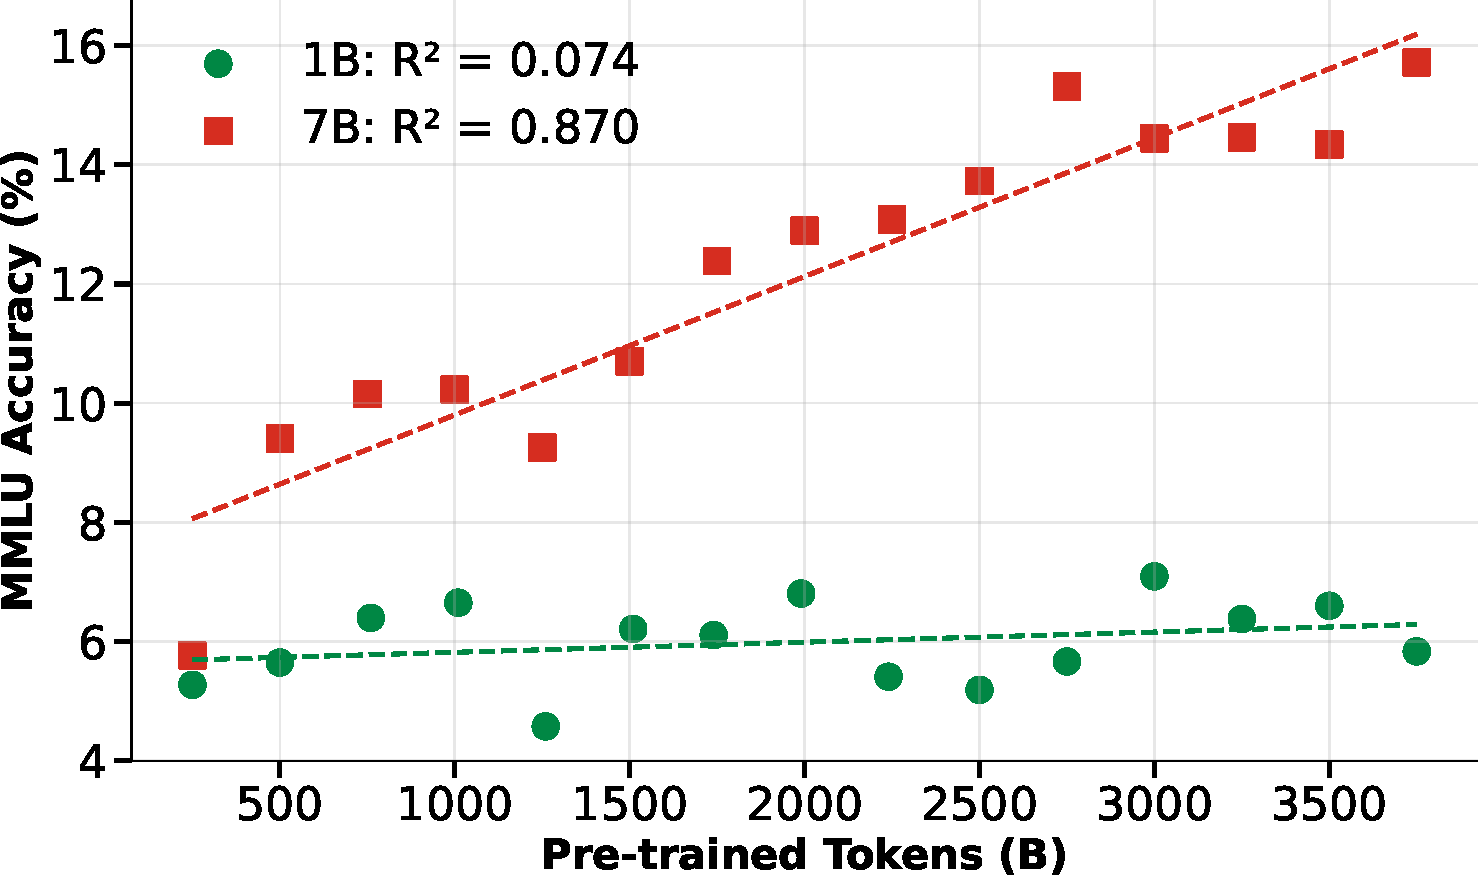
\includegraphics[width=\textwidth]{figs/mmlu_1b_7b_performance.pdf}
    \end{subfigure}
    \hfill
    \begin{subfigure}[b]{0.497\textwidth}
        \centering
        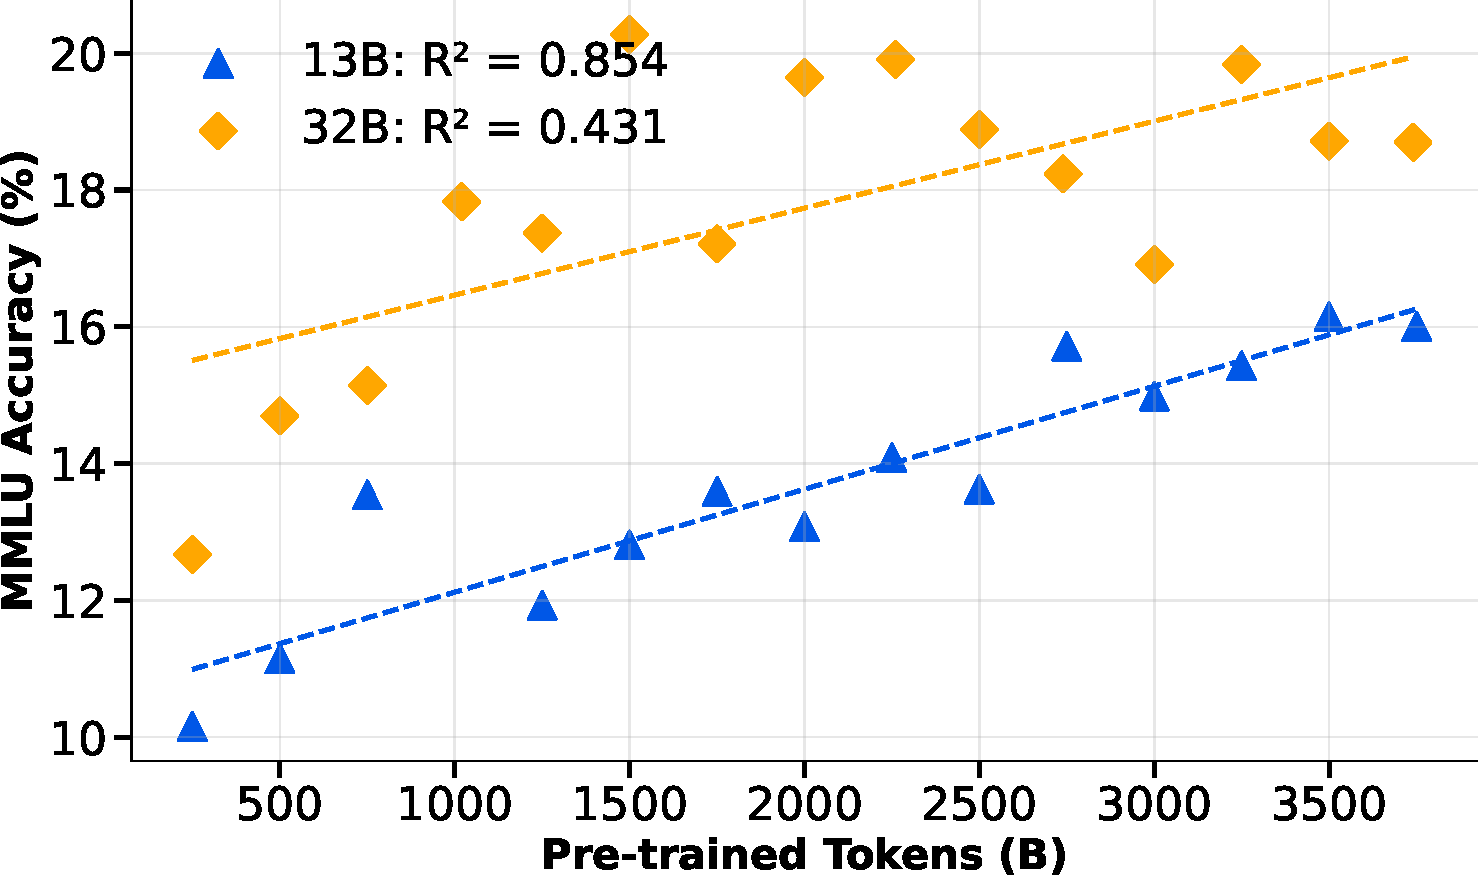
\includegraphics[width=\textwidth]{figs/mmlu_13b_32b_performance.pdf}
    \end{subfigure}
    
    \begin{subfigure}[b]{0.497\textwidth}
        \centering
        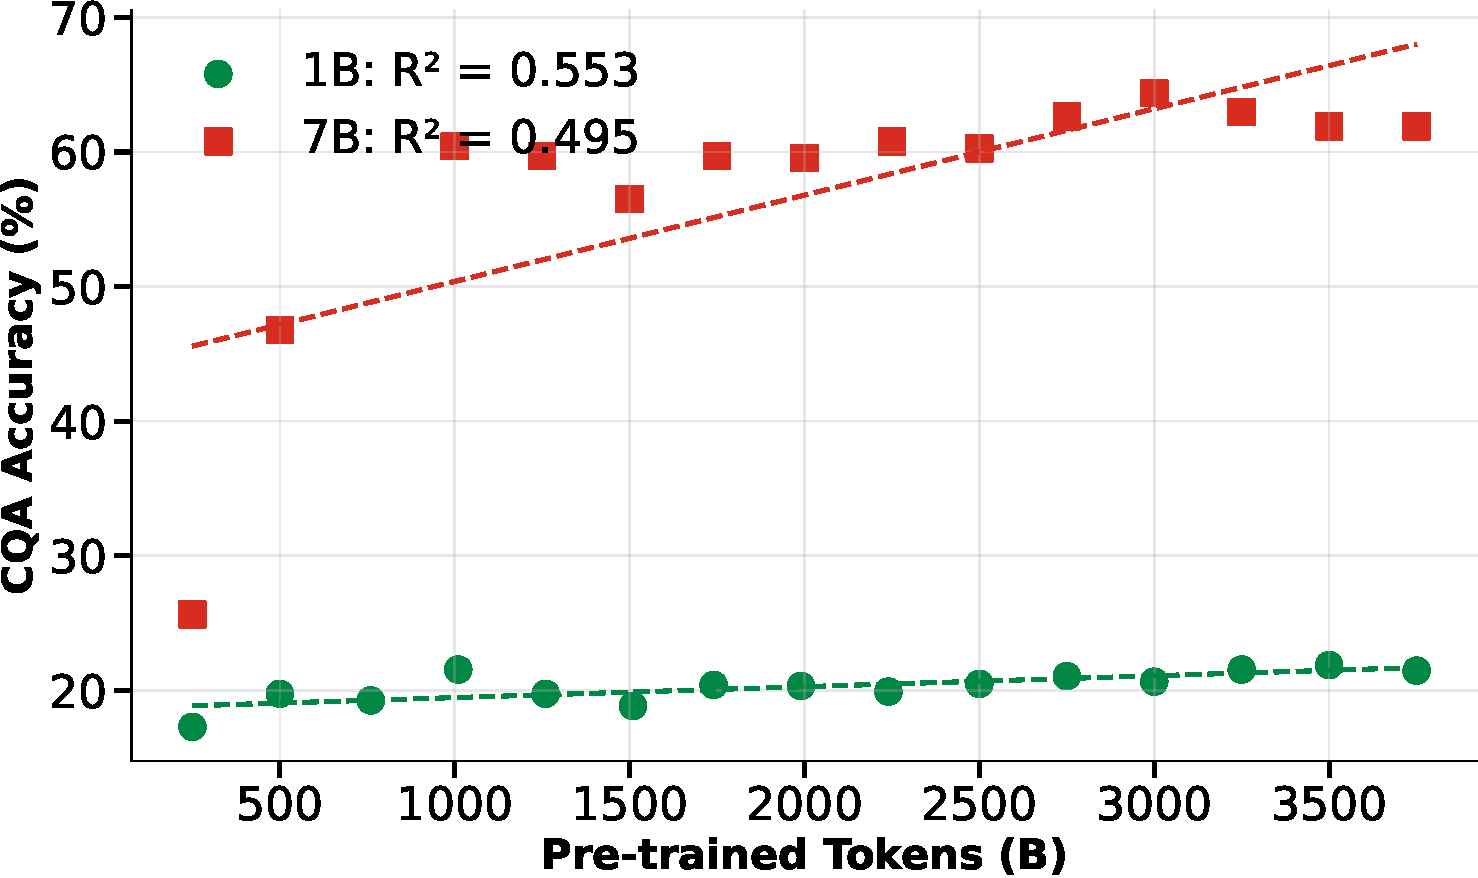
\includegraphics[width=\textwidth]{figs/cqa_1b_7b_performance.pdf}
    \end{subfigure}
    \hfill
    \begin{subfigure}[b]{0.497\textwidth}
        \centering
        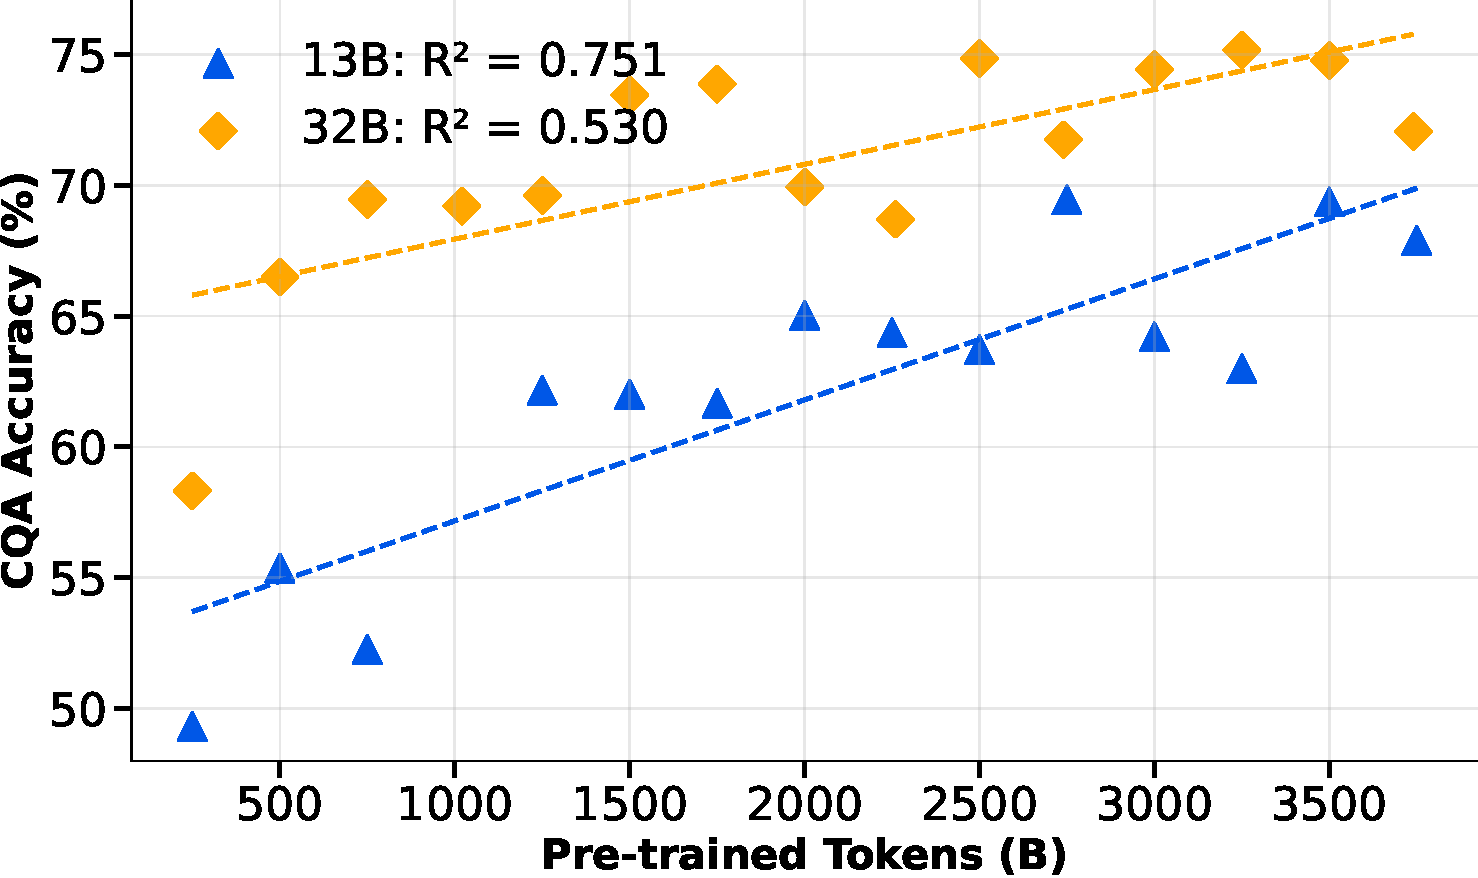
\includegraphics[width=\textwidth]{figs/cqa_13b_32b_performance.pdf}
    \end{subfigure}

\begin{subfigure}[b]{0.497\textwidth}
        \centering
        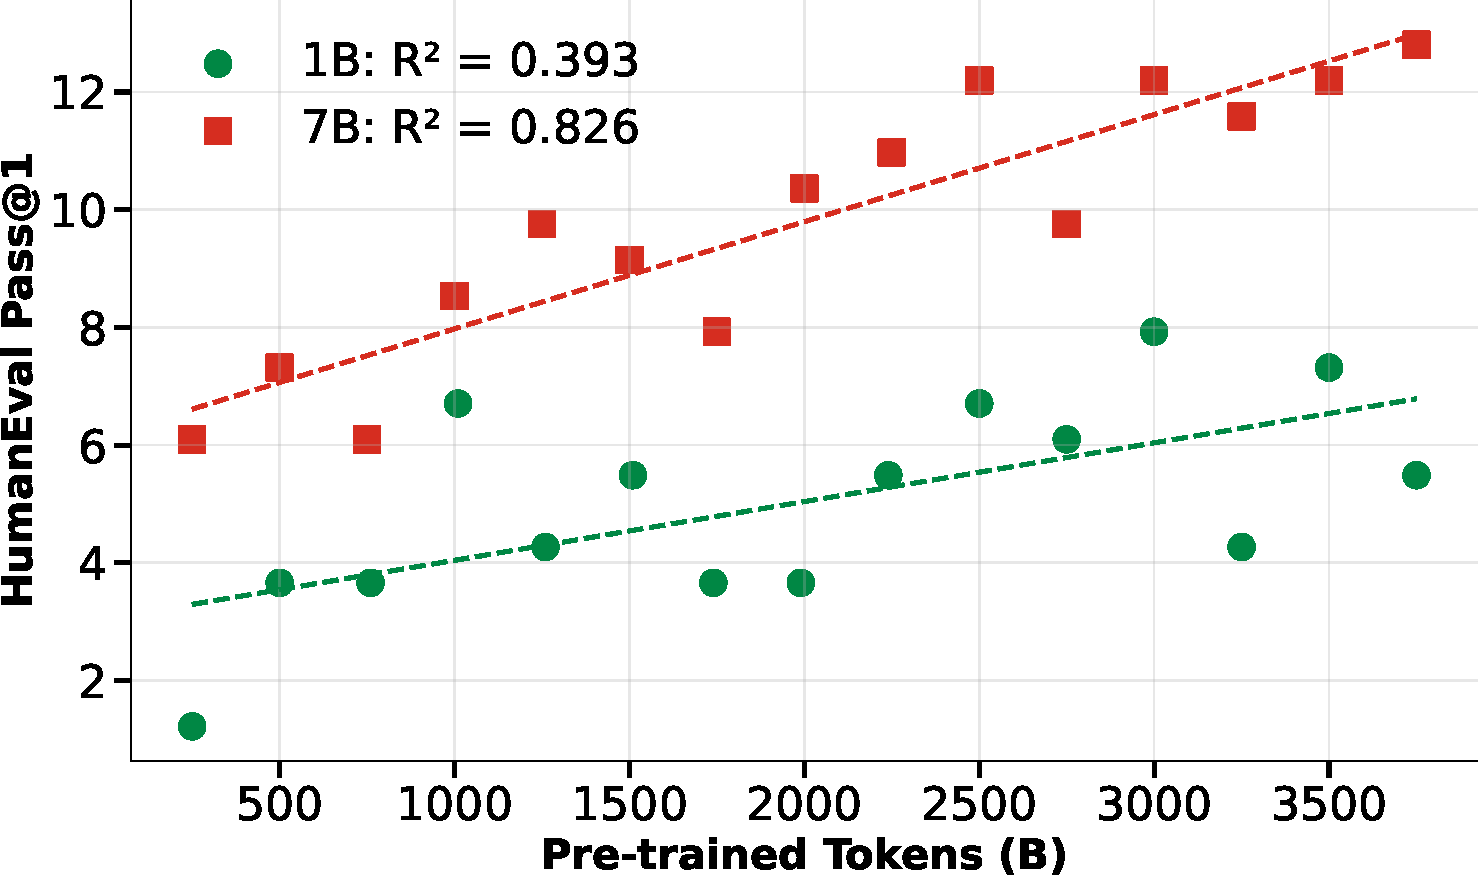
\includegraphics[width=\textwidth]{figs/humaneval_1b_7b_performance.pdf}
        \caption{Pre-training progress on 1B and 7B model}
    \end{subfigure}
    \hfill
    \begin{subfigure}[b]{0.497\textwidth}
        \centering
        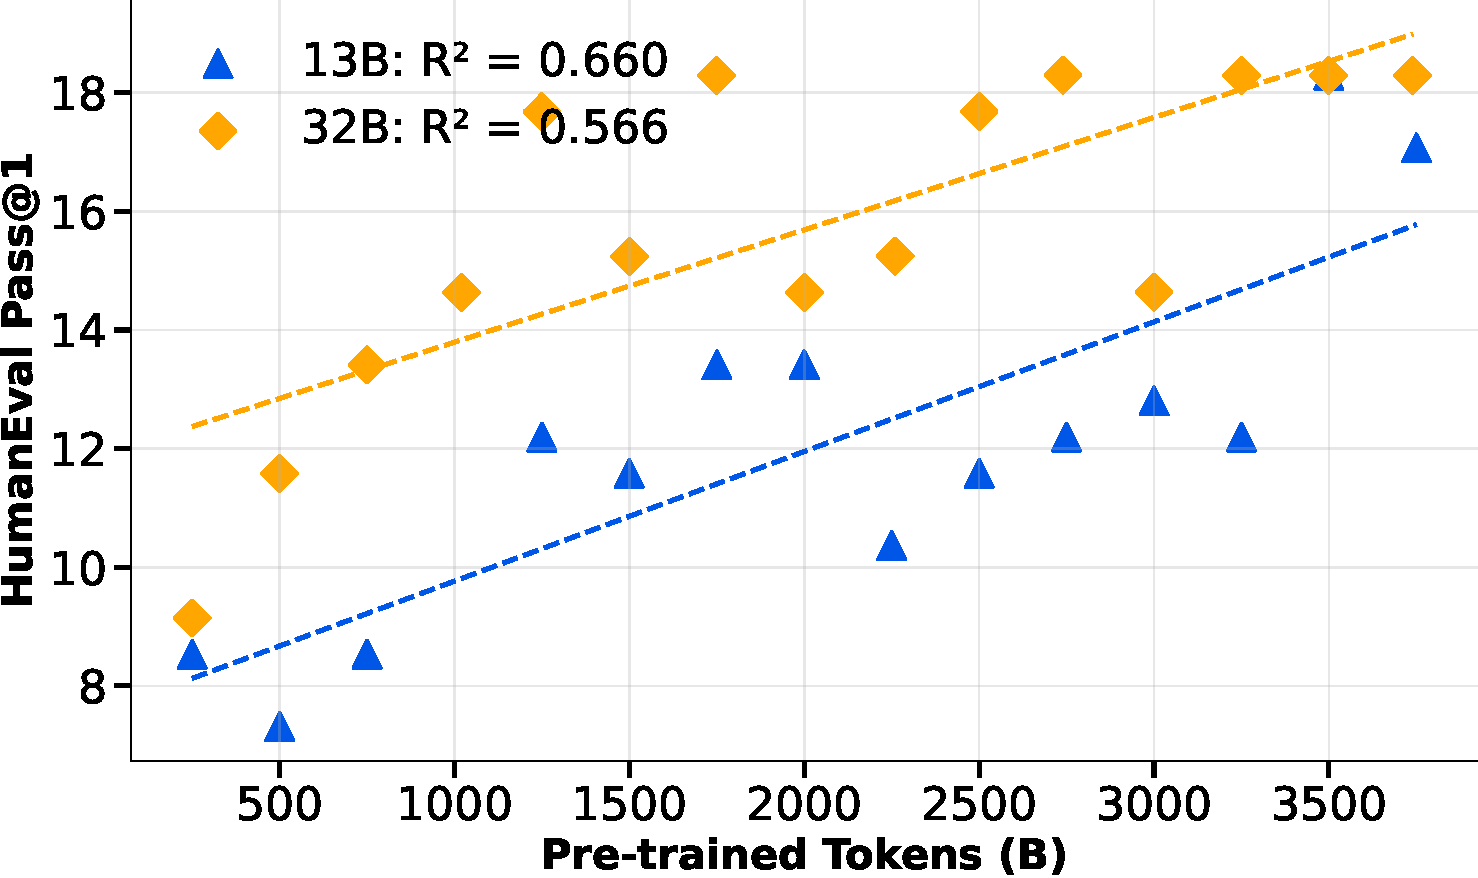
\includegraphics[width=\textwidth]{figs/humaneval_13b_32b_performance.pdf}
        \caption{Pre-training progress on 13B and 32B model}
    \end{subfigure}
    
    \caption{Given the same data source, smaller models exhibit significantly more noise and occasionally provide the wrong direction, making it challenging to use smaller models to proxy larger model performance. R$^2$ values are derived from linear curve fitting. MMLU corresponds to MMLU Pro (STEM).}
    \label{fig:motivation_app}
\end{figure}

\section{rBridge Pseudocode} \label{app:pseudocode}

\paragraph{Pseudocode.} The pseudocode is available in Alg. \ref{alg:rbridge}. We recommend viewing with Fig. \ref{fig:rbridge} to build intuition. Recall that $x$ is an input from the benchmark dataset's validation or test we want to evaluate. Recall that $\pi^\text{p}, \pi^\phi$ are the proxy, and frontier LMs, respectively. $i$ denotes index of token $\tau$. $\tau^\text{p}$ denotes the token tokenized using $\pi^\text{p}$'s tokenizer. Exact prompt and extraction used in Line 1 is available in \hyperlink{prompt}{prompt}.

\SetKwInput{Input}{Input}
\SetKwInput{Return}{Return}

\begin{algorithm2e}[H]
    \caption{\tsc{rBridge}}
    \label{alg:rbridge}
    \Input{$x, \pi^\text{p}, \pi^\phi$}
        \tcc{Step 1: Extract reasoning trace and token-level confidence from frontier model}
     $R^\phi, p(R^\phi) ,A^\phi \leftarrow \pi^\phi(x)$ \;

    \tcc{Step 2: Discard answer label, and compute normalized \tsc{rBridge} NLL}
    $w \leftarrow []$\;
    \For{\textnormal{\textbf{each} \textnormal{token} $\tau_i^\text{p}$ \textnormal{\textbf{tokenizing}} $R^\phi$}}{
       $w_i \leftarrow $\textnormal{Mean} $_{\text{letter} \in \tau_i^\text{p}}(p^\phi($\textnormal{letter}$)$ \textnormal{from} $p(R^\phi))$ \;
        $w.\text{append}(w_i)$
    }
    \tsc{rBridge} $\leftarrow []$\;
    \For{\textnormal{\textbf{each} \textnormal{token} $\tau_i^\text{p}$ \textnormal{\textbf{tokenizing}} $R^\phi$}}{
       $\textnormal{NLL} \leftarrow-\textnormal{log }p^\text{p}(\tau_i^\text{p}) \sim \pi^\text{p}$ \;
        \tsc{rBridge}.append$(\text{NLL}\cdot\frac{w[i]-\text{min}(w)}{\text{max}(w)-\text{min}(w)})$\;
    }
    \tsc{rBridge} $\leftarrow \text{Mean}(\tsc{rBridge})$\;
    \Return{\tsc{rBridge}}
\end{algorithm2e}


\paragraph{Prompt.} Here is the \hyperlink{prompt}{prompt} we use to generate $R^\phi$. We use greedy decoding. Brackets [] indicate dynamic insertions depending on the benchmark and question. We extract the value for key ``reasoning" to attain $R^\phi$.

\hypertarget{prompt}{}
\begin{tcolorbox}[colback=gray!5!white, colframe=gray!75!black, title=Prompt to Frontier Model, label={box:mailman_question}]

System: You are a helpful assistant that solves [task] problems.

\vspace{1em}

User: [question]

Respond ONLY with a JSON object in this exact format:
\{ ``reasoning": ``your step by step reasoning", ``final\_answer": ``your final answer" \}

\end{tcolorbox}

\section{Further Experimental Details} \label{app:setting}

\paragraph{Common Evaluation Setting.} All evaluations are done using 5-shot CoT \citep{NEURIPS2022_9d560961}.

\subsection{Hardware} We use A100 80G, H100 and H200 nodes and numerous terabytes of disk storage for experiments. For pre-training, we use 256 H100 GPUs with HBM3. For other hardware like CPU and RAM we use commonly available ones, as these hardware did not induce any bottlenecks. 


\subsection{Experiment (i) Additional Details} All proxy models used is the default seed as provided in \cite{magnusson2025datadecide}. We do not use multi-seed averaging for the proxy as this significantly increases compute cost. We exactly follow  \cite{magnusson2025datadecide} on every other aspect of experiments, using their open-source assets where available. All intermediary checkpoints are as available from \cite{magnusson2025datadecide}.

\subsection{Experiment (ii) Additional Details} 

\paragraph{Additional Baseline Details.} iSFT results are unavailable for MMLU Pro (STEM) and HumanEval as these benchmarks do not provide an SFT set.

\paragraph{Frontier Model's $R^\phi$.} Following \cite{team2025minicpm4}, we use \ttt{GPT 4o} to generate $R^\phi$. We tested \ttt{Claude 3.5 Sonnet} and \ttt{Gemini 2.5 Pro} and found no meaningful performance difference. We have not tested this method on long CoT models.

\paragraph{Pre-training and Post-training Details.} Unless stated otherwise, for pre-training, we fully follow OLMo 2 \citep{olmo20242}, and use their checkpoints where available. For SFT post-training we use the settings in Tab. \ref{tab:hyperparams}.

\begin{table}[ht]
    \centering
    \caption{Hyperparameters for SFT}
    \label{tab:hyperparams}
    \resizebox{0.4\columnwidth}{!}{
        \begin{tabular}{lc}
        \toprule
        \textbf{Hyperparameter} & \textbf{Value} \\
        \midrule
        Epoch & 1 \\
        Learning Rate & $1 \times 10^{-5}$ \\
        Warmup Ratio & 0.1 \\
        Batch Size & 64 \\
        \bottomrule
        \end{tabular}
    }
\end{table}

\subsection{Experiment (iii) Additional Details} 

\paragraph{Alternative Pre-training Dataset $\mc{D}'$.} For the alternative pre-training dataset $\mc{D}'$  described in experiment \textbf{(iii)}, we closely follow the setup described in \cite{han2025trillion}, but exclusively use publicly-available datasets. The training data follows an 8.5:1:0.5 ratio of English:multilingual:math/code, where the English portion consists of DCLM and FineWeb-Edu in equal proportions, and the multilingual portion comprises Korean, Chinese, and Japanese dumps of FineWeb and DCLM pipeline-processed Common Crawl filtered for Korean. 

\paragraph{Benchmark Choice.} We use the same benchmarks presented in \textbf{(ii)}, excluding HumanEval, as our extraction method on the alternative dataset $\mc{D}'$ achieved 0\% p@1.

\section{Additional Experimental Results} \label{app:more_exp}

Refer to Fig. \ref{fig:curve_fit} and \ref{fig:curve_fit_1} for extended curve fitting visualization examples. Refer to Tab. \ref{tab:olmo_1b_13b_pre_to_post} for all 1B $\rightarrow$ 13B (Pre-to-Post) benchmark results. MMLU Pro (STEM) and HumanEval are not included as they do not have a designated SFT set. Refer to Tab. \ref{tab:olmo_1b_32b_pre_to_pre} for all 1B $\rightarrow$ 32B (Pre-to-Pre) benchmark results. Refer to Fig. \ref{fig:kendall} for Kendall Tau results.

\begin{figure}[tb!]
    \centering
    \begin{subfigure}[b]{0.497\textwidth}
        \centering
        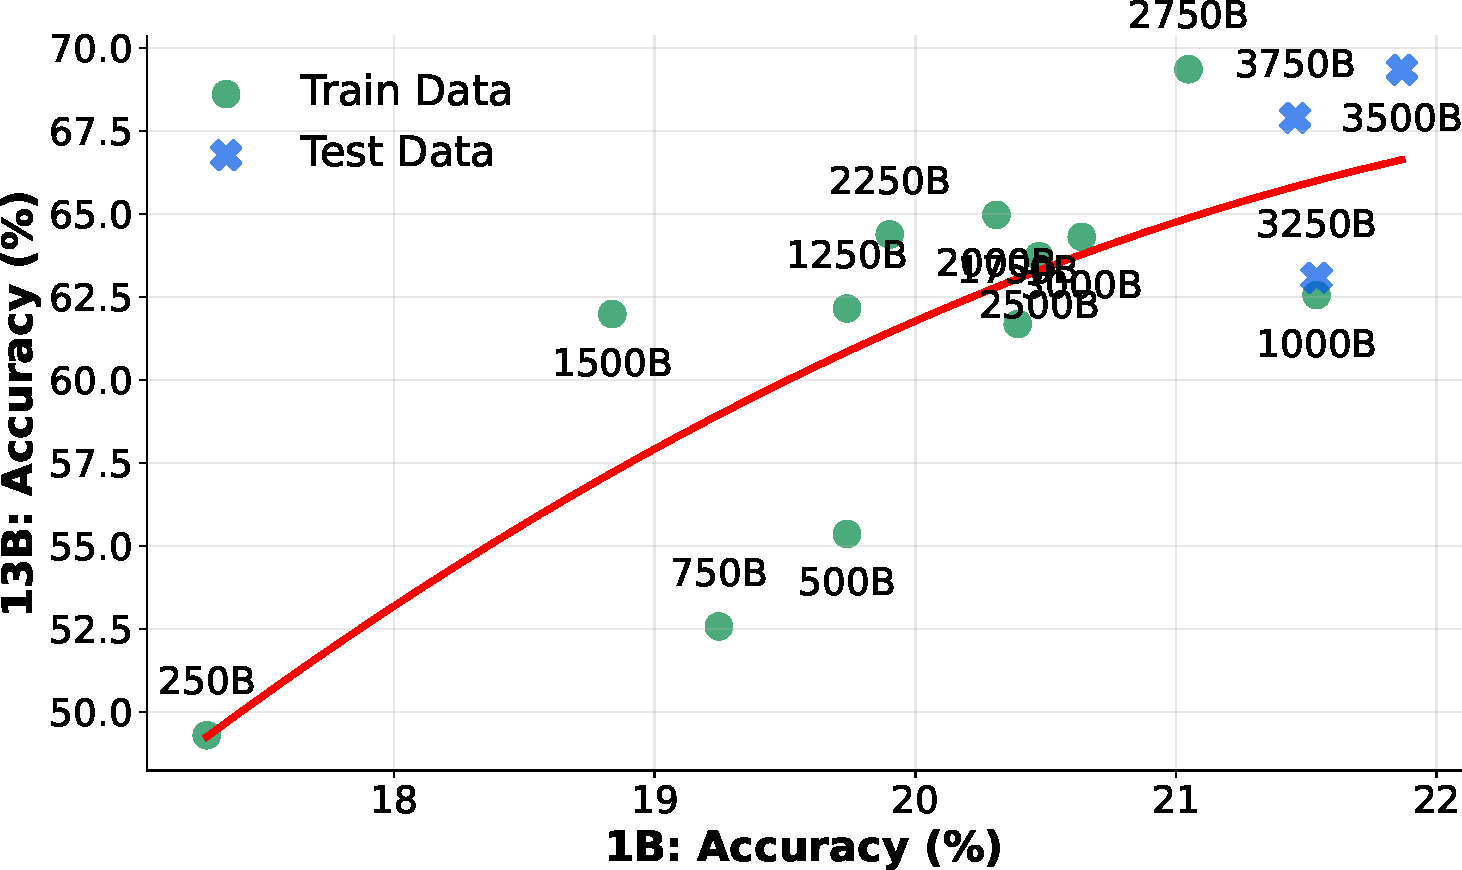
\includegraphics[width=\textwidth]{figs/cqa_acc.pdf}
        \caption{Target metric Acc. as the proxy metric at 1B on CQA.}
    \end{subfigure}
    \hfill
    \begin{subfigure}[b]{0.497\textwidth}
        \centering
        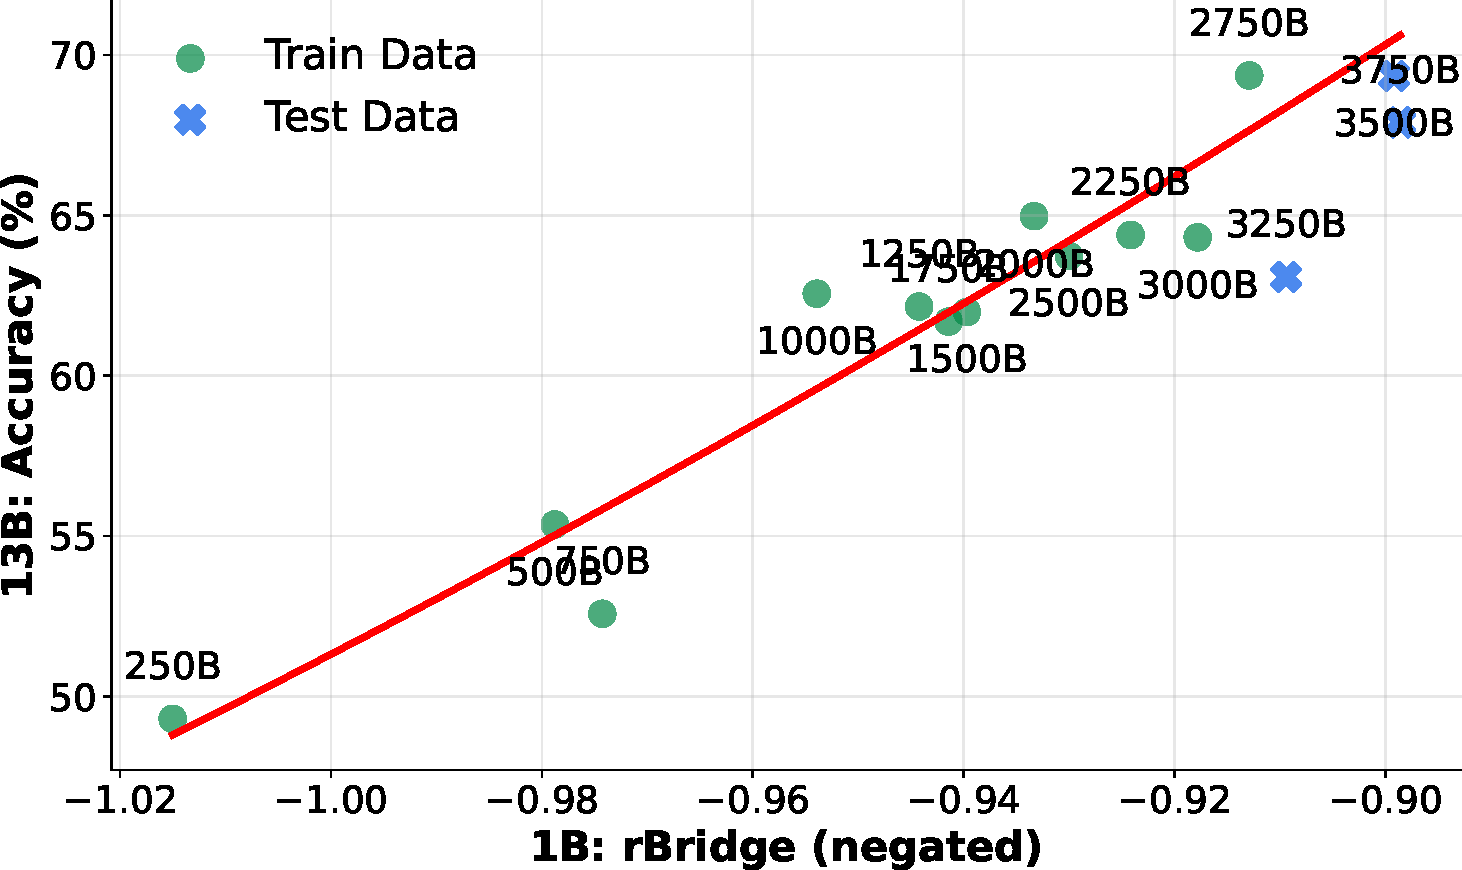
\includegraphics[width=\textwidth]{figs/cqa_rbridge.pdf}
        \caption{\tsc{rBridge} as the proxy metric at 1B on CQA.\\~\\}
    \end{subfigure}

    \begin{subfigure}[b]{0.497\textwidth}
        \centering
        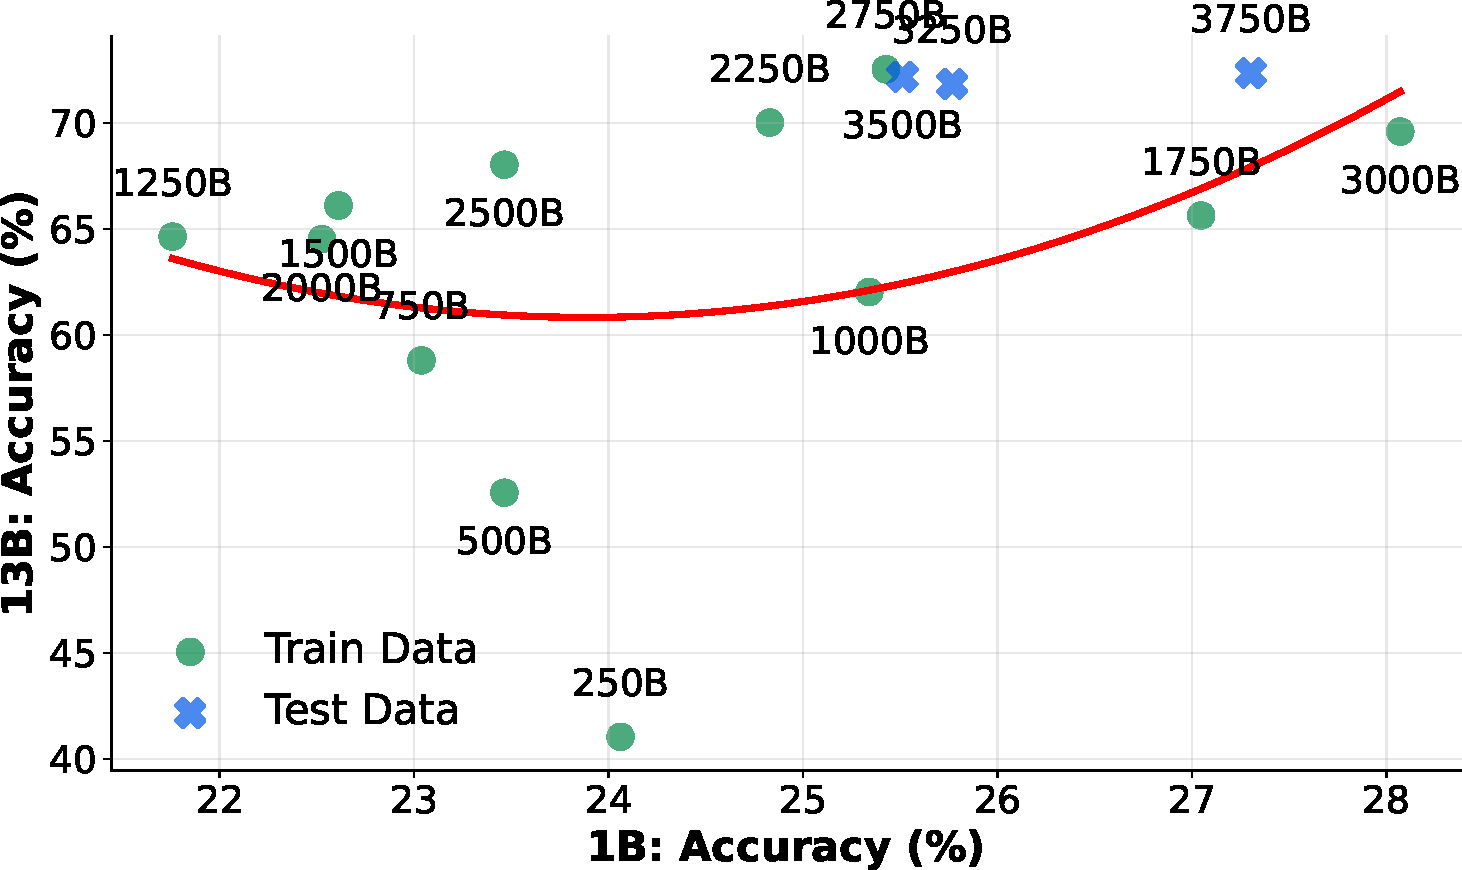
\includegraphics[width=\textwidth]{figs/arc-c_acc.pdf}
        \caption{Target metric Acc. as the proxy metric at 1B on ARC-C.}
    \end{subfigure}
    \hfill
    \begin{subfigure}[b]{0.497\textwidth}
        \centering
        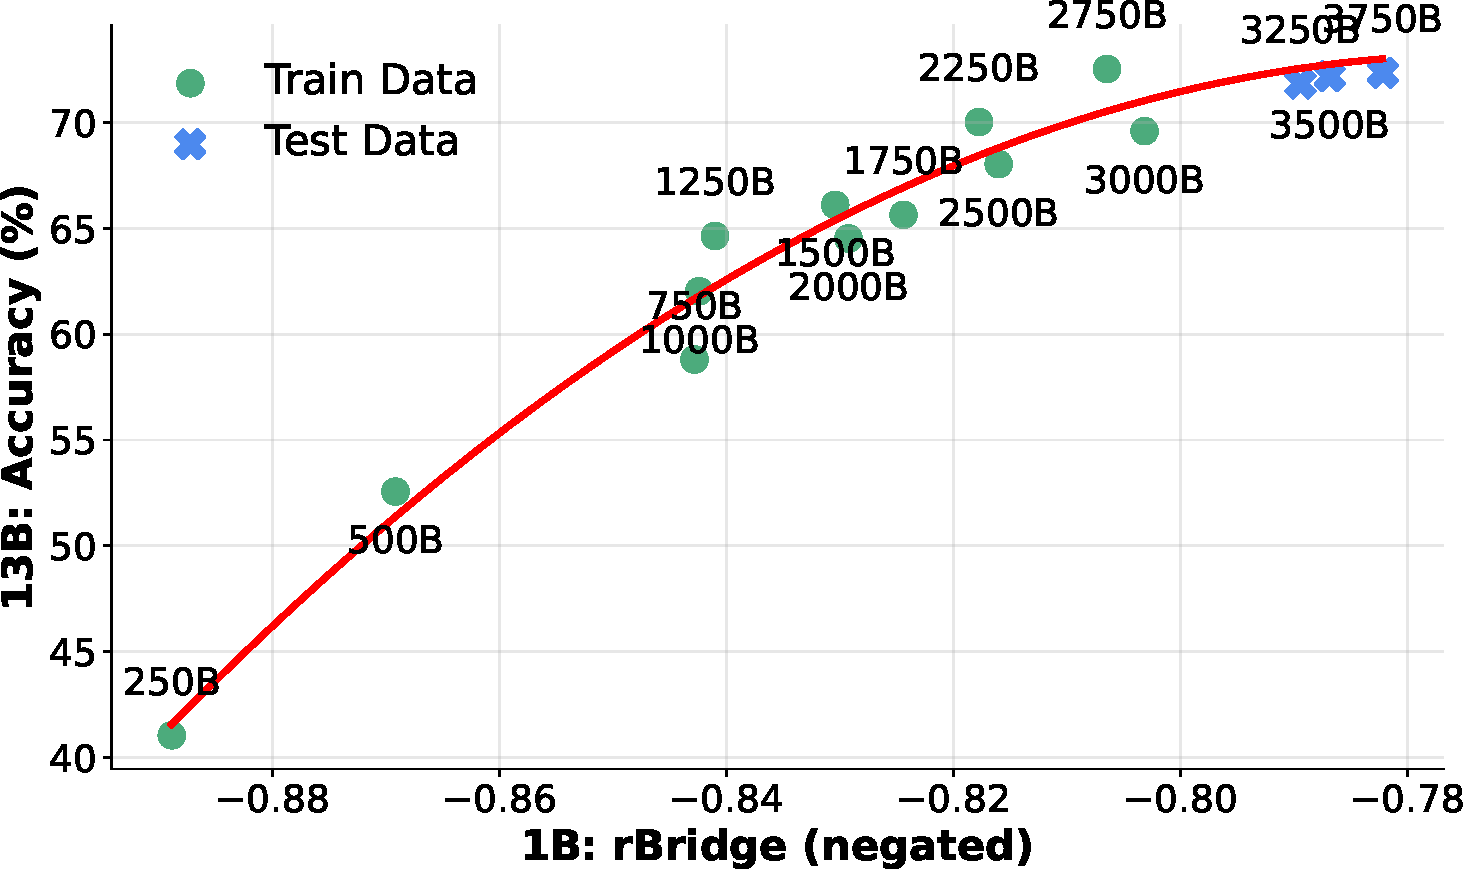
\includegraphics[width=\textwidth]{figs/arc-c_rbridge.pdf}
        \caption{\tsc{rBridge} as the proxy metric at 1B on ARC-C.\\~\\}
    \end{subfigure}

    \begin{subfigure}[b]{0.497\textwidth}
        \centering
        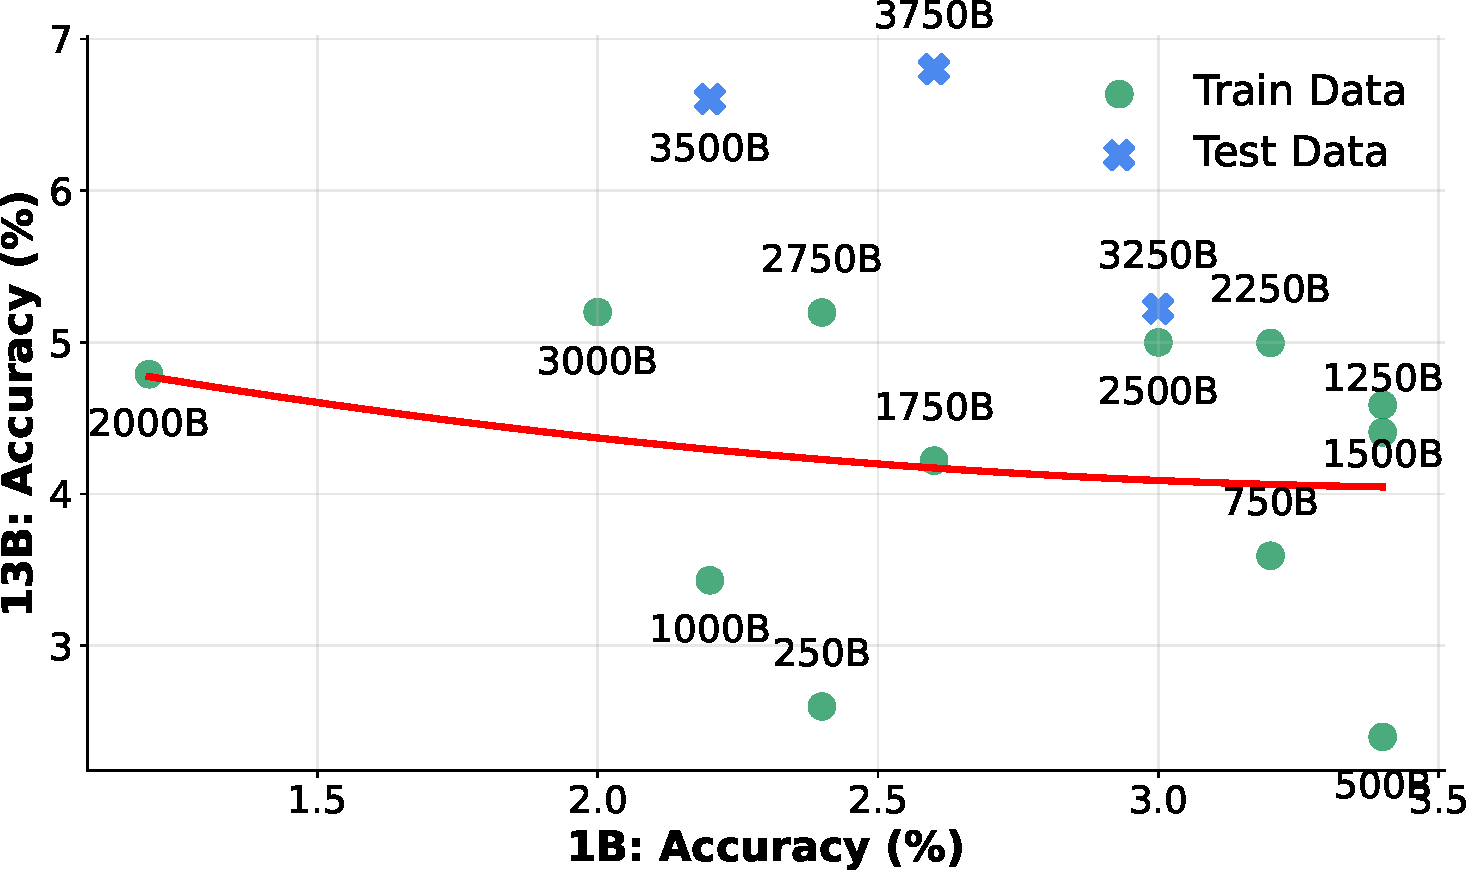
\includegraphics[width=\textwidth]{figs/math500_acc.pdf}
        \caption{Target metric Acc. as the proxy metric at 1B on MATH500.}
    \end{subfigure}
    \hfill
    \begin{subfigure}[b]{0.497\textwidth}
        \centering
        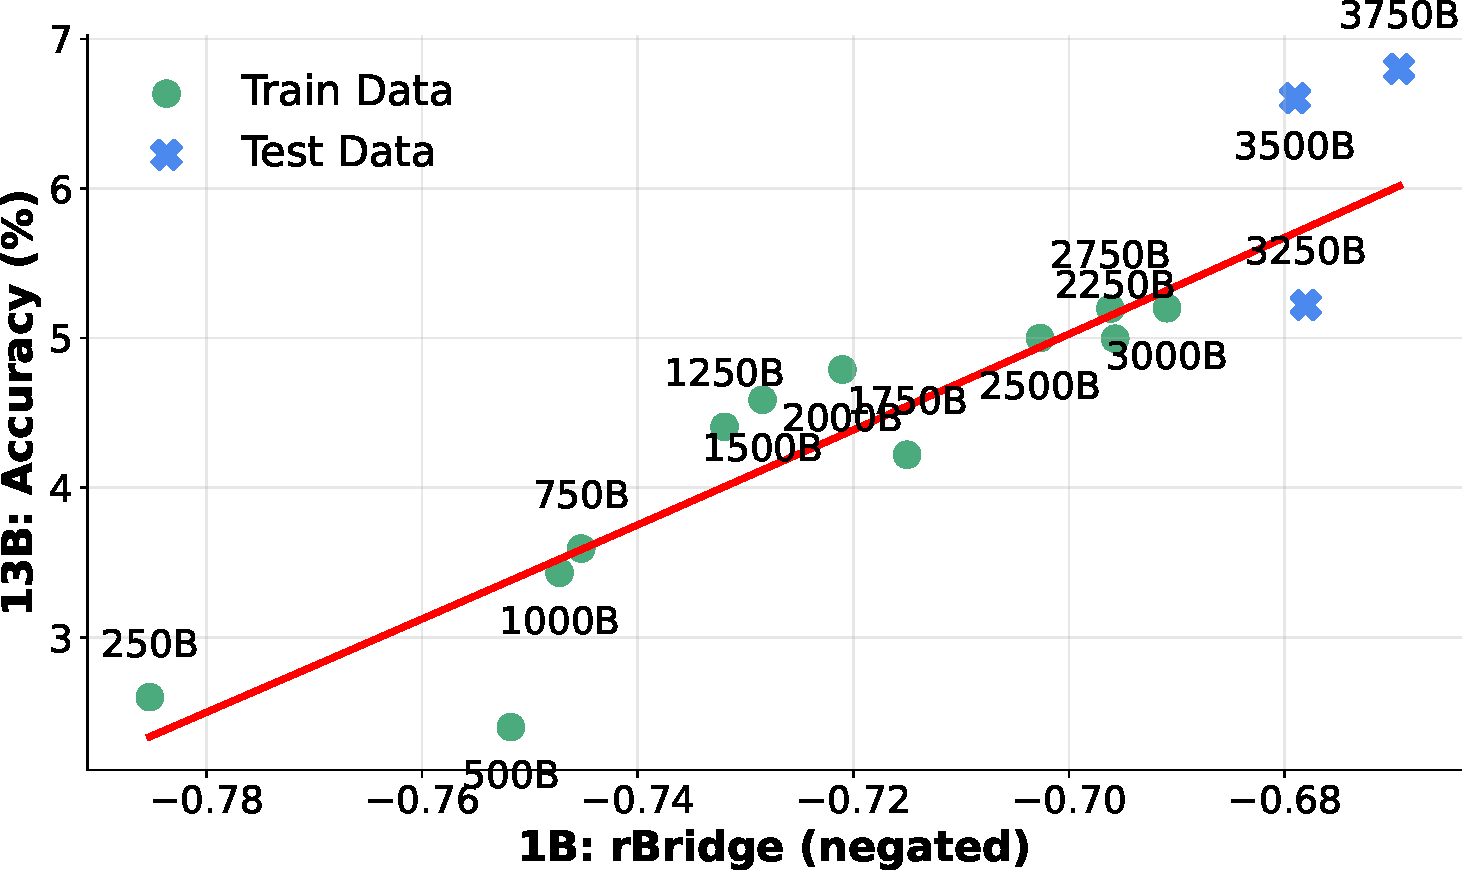
\includegraphics[width=\textwidth]{figs/math500_rbridge.pdf}
        \caption{\tsc{rBridge} as the proxy metric at 1B on MATH500.\\~\\}
    \end{subfigure}

        \begin{subfigure}[b]{0.497\textwidth}
        \centering
        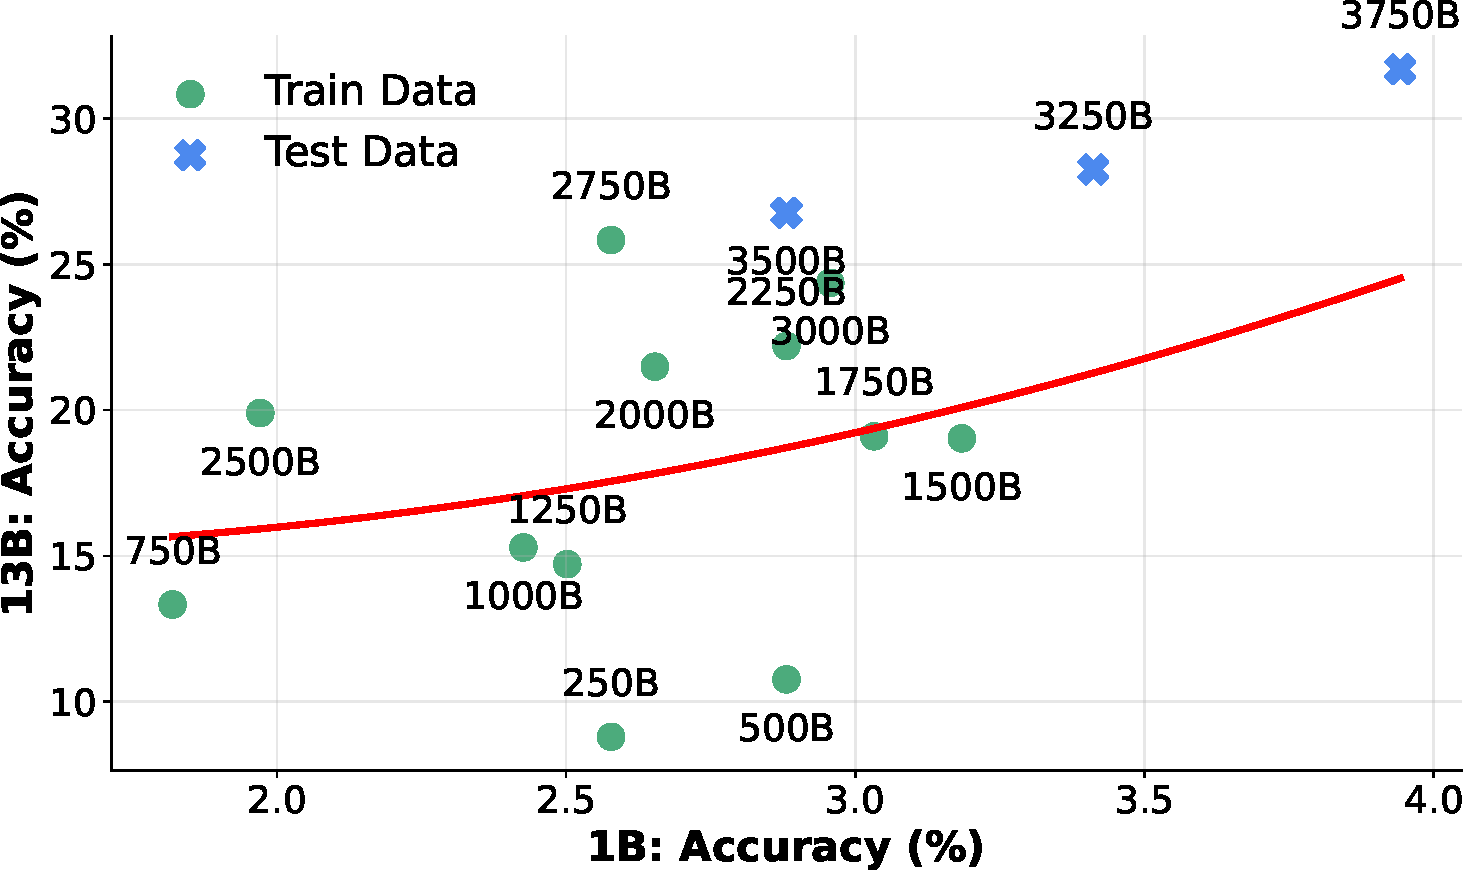
\includegraphics[width=\textwidth]{figs/gsm8k_acc.pdf}
        \caption{Target metric Acc. as the proxy metric at 1B on GSM8K.}
    \end{subfigure}
    \hfill
    \begin{subfigure}[b]{0.497\textwidth}
        \centering
        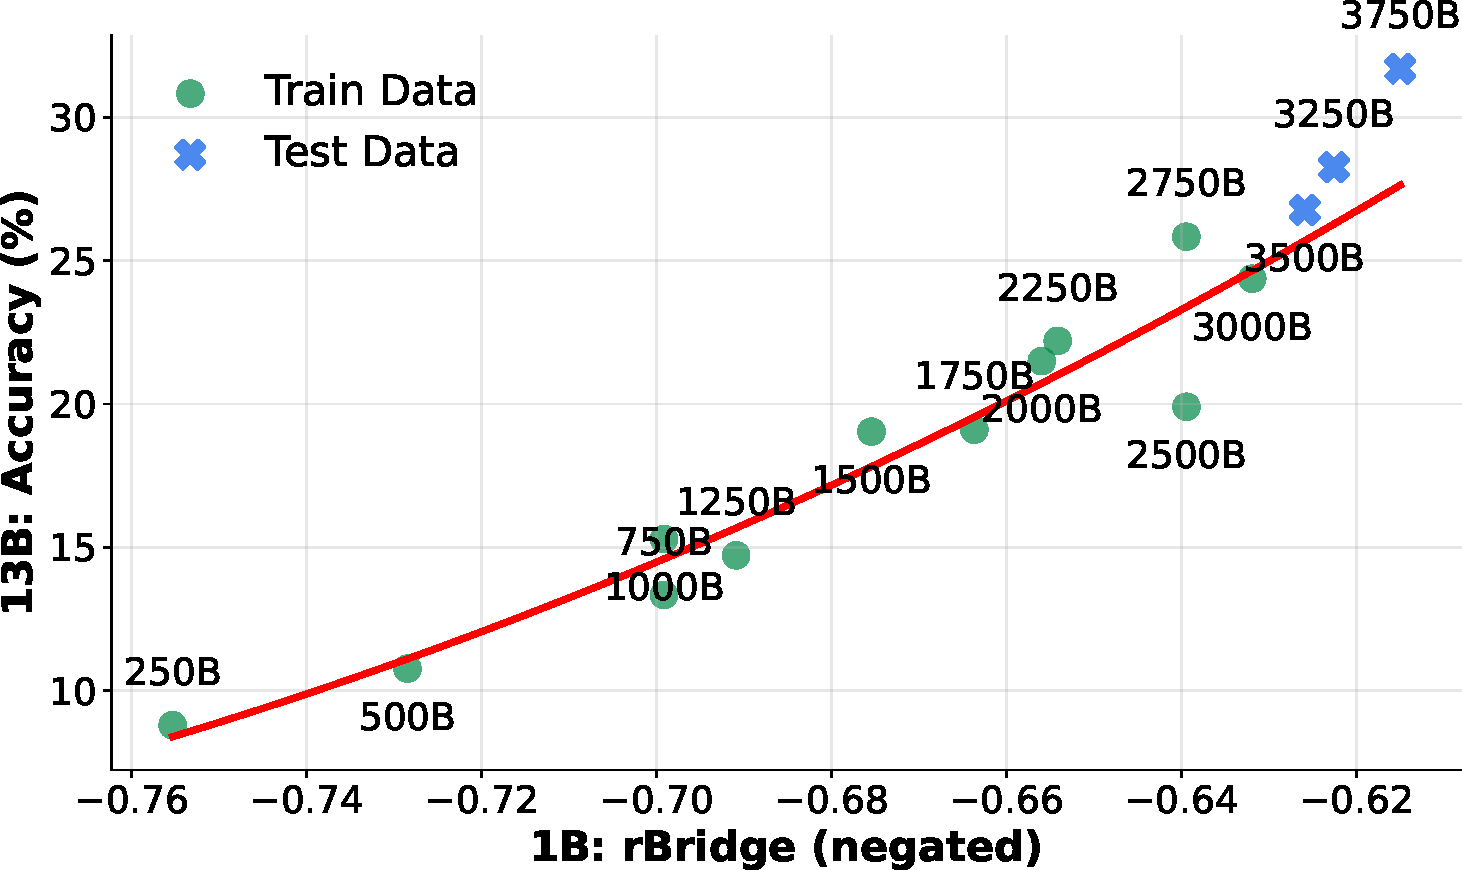
\includegraphics[width=\textwidth]{figs/gsm8k_rbridge.pdf}
        \caption{\tsc{rBridge} as the proxy metric at 1B on GSM8K.\\~\\}
    \end{subfigure}

    \caption{Example visualization from a fold of proxy-target relationship study at 1B $\rightarrow$ 13B on CQA, ARC-C, MATH500, and GSM8K. Each data point represents equal trained tokens for the proxy and target model.}
    \label{fig:curve_fit}
\end{figure}

\begin{figure}[tb!]
    \centering
            \begin{subfigure}[b]{0.497\textwidth}
        \centering
        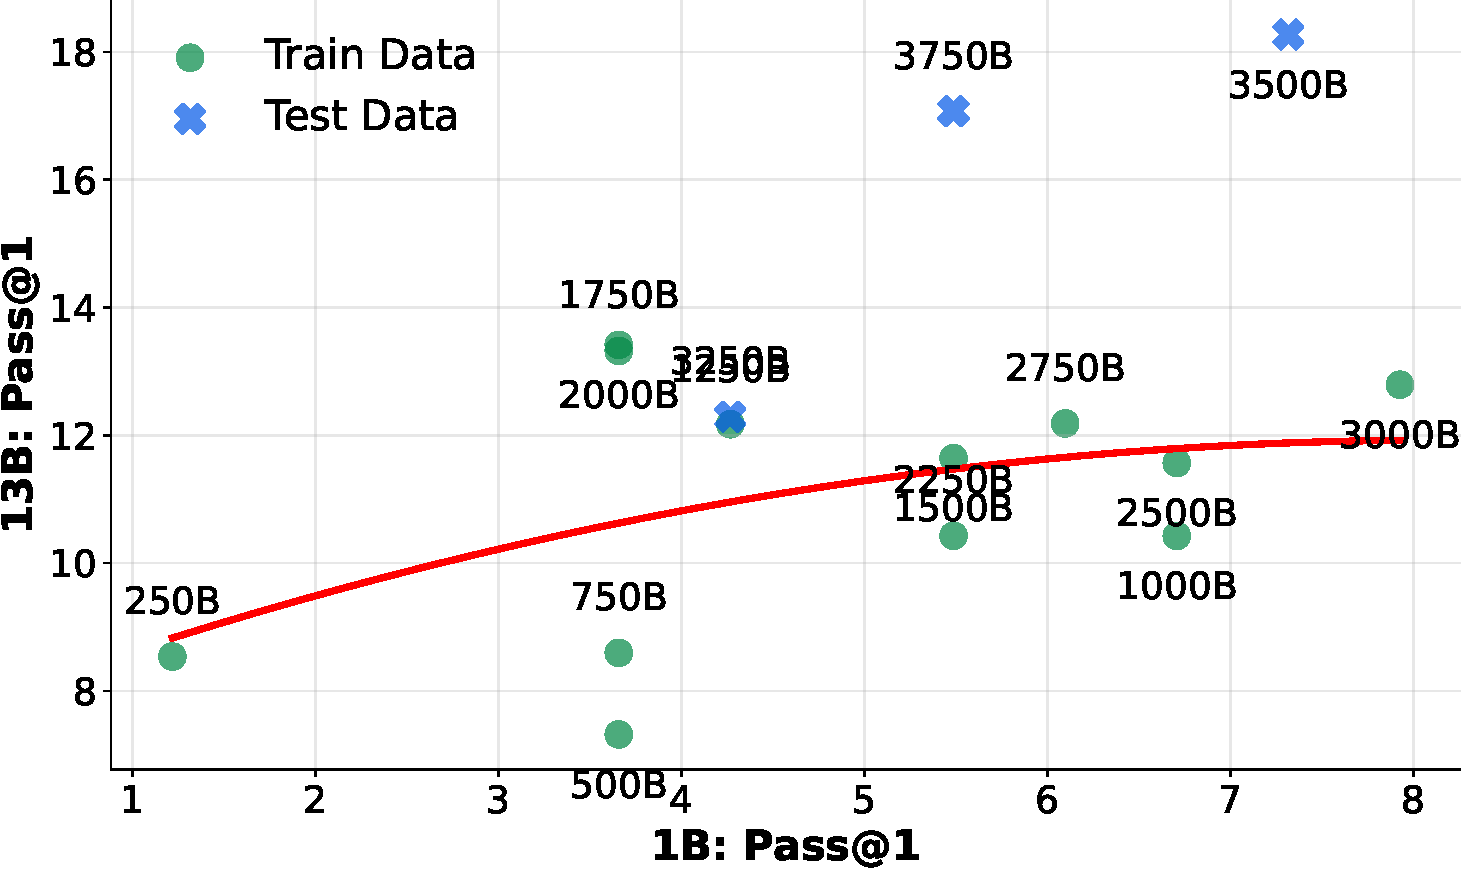
\includegraphics[width=\textwidth]{figs/humaneval_pass_1.pdf}
        \caption{Target metric Acc. as the proxy metric at 1B.}
    \end{subfigure}
    \hfill
    \begin{subfigure}[b]{0.497\textwidth}
        \centering
        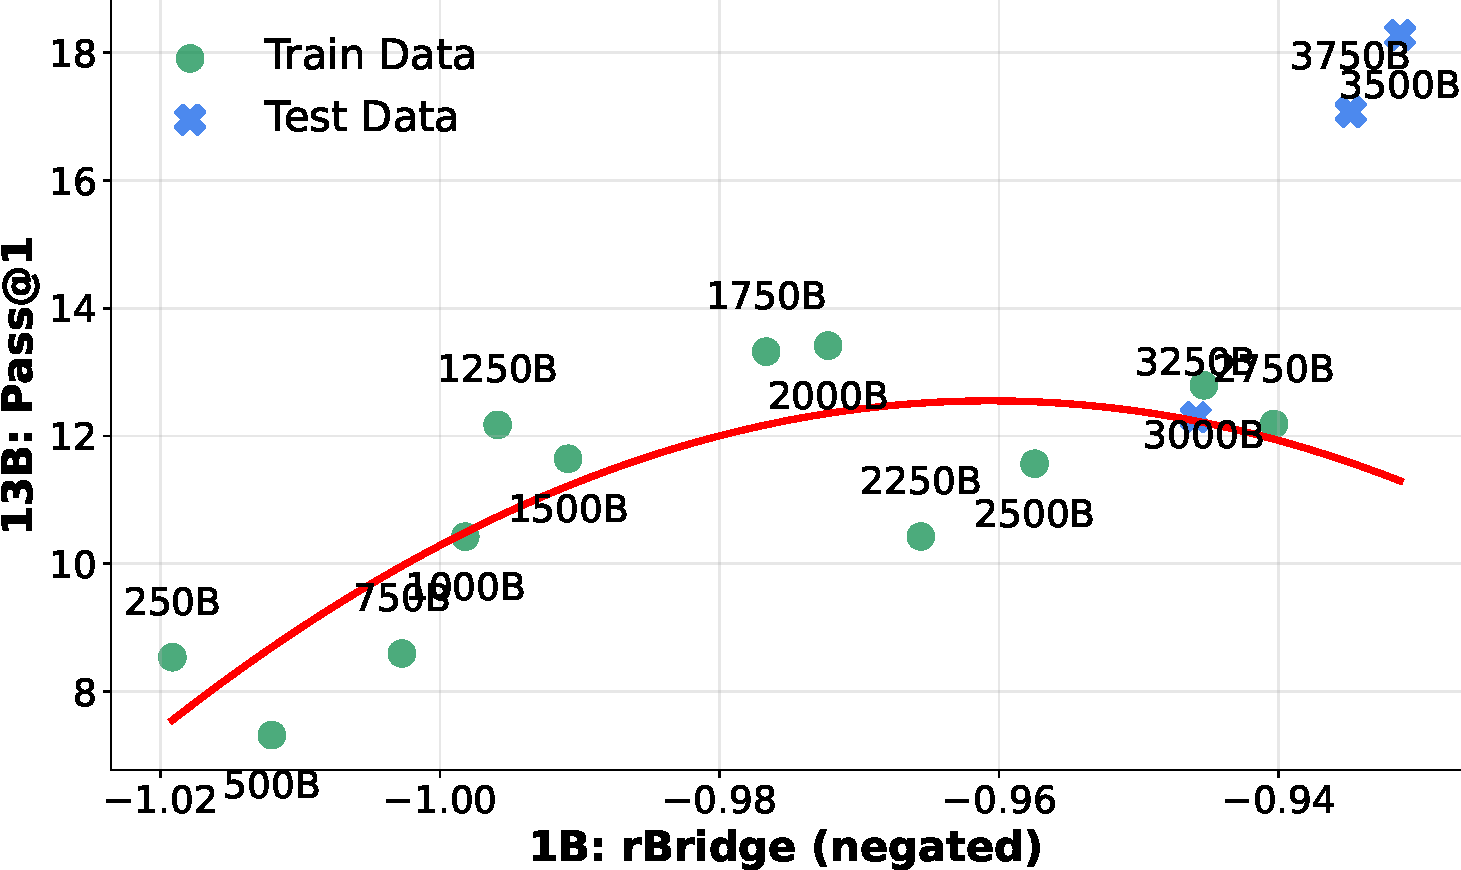
\includegraphics[width=\textwidth]{figs/humaneval_rbridge.pdf}
        \caption{\tsc{rBridge} as the proxy metric at 1B.}
    \end{subfigure}
    
    \caption{Example visualization from a fold of proxy-target relationship study at 1B $\rightarrow$ 13B on HumanEval. Each data point represents equal trained tokens for the proxy and target model.}
    \label{fig:curve_fit_1}
\end{figure}


\begin{table*}[htbp]
\centering
\resizebox{\textwidth}{!}{
\begin{tabular}{llcccccc>{\columncolor{gray!15}}c}
\toprule
\textbf{Benchmark} & \textbf{Method:} & \textbf{Acc./p@1} & \textbf{iSFT} & \textbf{TED} & \textbf{MPCA} & \textbf{NLL} & \textbf{$R^\phi$} & \textbf{\texttt{rBridge}} \\
\midrule
\multirow{2}{*}{GSM8K} & Train R$^2$ & 0.363 & 0.385 & 0.565 & 0.129 & 0.868 & \underline{0.951} & \textbf{0.956} \\
 & Test MAE & 5.807 & 5.536 & 7.054 & 79.761 & 3.302 & \underline{1.715} & \textbf{1.616} \\
\midrule
\multirow{2}{*}{MATH500} & Train R$^2$ & 0.088 & 0.128 & 0.199 & 0.182 & \textbf{0.557} & 0.544 & \underline{0.555} \\
 & Test MAE & 1.178 & 0.888 & 0.805 & 0.849 & 0.692 & \underline{0.609} & \textbf{0.605} \\
\midrule
\multirow{2}{*}{ARC-C} & Train R$^2$ & 0.187 & 0.153 & 0.522 & 0.331 & 0.160 & \underline{0.938} & \textbf{0.964} \\
 & Test MAE & 6.921 & 8.317 & 6.248 & 22.685 & 6.679 & \underline{1.590} & \textbf{1.279} \\
\midrule
\multirow{2}{*}{CQA} & Train R$^2$ & 0.677 & 0.543 & 0.783 & 0.385 & 0.068 & \underline{0.845} & \textbf{0.910} \\
 & Test MAE & 3.593 & 6.264 & 2.837 & 4.952 & 5.055 & \underline{2.283} & \textbf{1.715} \\
\midrule
\multicolumn{2}{l}{\textbf{Average Train R$^2$ ($\uparrow$)}} & 0.329 & 0.302 & 0.517 & 0.257 & 0.413 & \underline{0.820} & \textbf{0.846} \\
\multicolumn{2}{l}{\textbf{Average Test MAE ($\downarrow$)}} & 4.375 & 5.251 & 4.236 & 27.062 & 3.932 & \underline{1.549} & \textbf{1.304} \\
\bottomrule
\end{tabular}}
\caption{Detailed results of 1B $\rightarrow$ 13B+SFT (Pre-to-Post). Train fitting and test is done using 5-fold cross validation (\textbf{\S\ \ref{sec:protocol}}). Best value across methods is \textbf{bolded}, and second best is \underline{underlined}.}
\label{tab:olmo_1b_13b_pre_to_post}
\end{table*}

\begin{table*}[htbp]
\centering
\resizebox{\textwidth}{!}{
\begin{tabular}{llcccccc>{\columncolor{gray!15}}c}
\toprule
\textbf{Benchmark} & \textbf{Method:} & \textbf{Acc./p@1} & \textbf{iSFT} & \textbf{TED} & \textbf{MPCA} & \textbf{NLL} & \textbf{$R^\phi$} & \textbf{\texttt{rBridge}} \\
\midrule
\multirow{2}{*}{GSM8K} & Train R$^2$ & 0.281 & 0.398 & 0.706 & 0.076 & \underline{0.814} & \textbf{0.972} & \textbf{0.972} \\
 & Test MAE & 7.755 & 7.299 & 6.505 & 107.493 & 6.935 & \underline{1.676} & \textbf{1.601} \\
\midrule
\multirow{2}{*}{MATH500} & Train R$^2$ & 0.193 & 0.196 & 0.166 & 0.019 & 0.823 & \underline{0.832} & \textbf{0.834} \\
 & Test MAE & 98.093 & 1.869 & 1.985 & 6.907 & 0.815 & \underline{0.739} & \textbf{0.718} \\
\midrule
\multirow{2}{*}{ARC-C} & Train R$^2$ & 0.206 & 0.169 & 0.582 & 0.346 & 0.144 & \underline{0.926} & \textbf{0.949} \\
 & Test MAE & 4.734 & 5.976 & 4.491 & 7.588 & 4.985 & \underline{1.560} & \textbf{1.384} \\
\midrule
\multirow{2}{*}{\makecell{MMLU Pro\\(STEM)}} & Train R$^2$ & 0.057 & --- & 0.031 & 0.210 & \underline{0.344} & \textbf{0.756} & \textbf{0.756} \\
 & Test MAE & 2.075 & --- & 1.930 & \underline{1.864} & 2.133 & \textbf{1.326} & \textbf{1.326} \\
\midrule
\multirow{2}{*}{CQA} & Train R$^2$ & 0.624 & 0.634 & 0.528 & 0.332 & 0.046 & \underline{0.765} & \textbf{0.766} \\
 & Test MAE & 4.105 & 5.516 & 3.630 & 4.199 & 3.664 & \textbf{2.382} & \underline{2.384} \\
\midrule
\multirow{2}{*}{HumanEval} & Train R$^2$ & 0.514 & --- & 0.101 & 0.245 & \textbf{0.759} & 0.666 & \underline{0.679} \\
 & Test MAE & 1.946 & --- & 2.733 & 2.947 & \textbf{1.424} & 1.555 & \underline{1.474} \\
\midrule
\multicolumn{2}{l}{\textbf{Average Train R$^2$ ($\uparrow$)}} & 0.312 & 0.349 & 0.352 & 0.205 & 0.488 & \underline{0.820} & \textbf{0.826} \\
\multicolumn{2}{l}{\textbf{Average Test MAE ($\downarrow$)}} & 19.785 & 5.165 & 3.546 & 21.833 & 3.276 & \underline{1.540} & \textbf{1.481} \\
\bottomrule
\end{tabular}}
\caption{Detailed results of 1B $\rightarrow$ 32B (Pre-to-Pre). Train fitting and test is done using 5-fold cross validation (\textbf{\S\ \ref{sec:protocol}}). Best value across methods is \textbf{bolded}, and second best is \underline{underlined}.}
\label{tab:olmo_1b_32b_pre_to_pre}
\end{table*}

\begin{figure}[tb]
    \centering
    \begin{subfigure}[b]{0.497\textwidth}
        \centering
        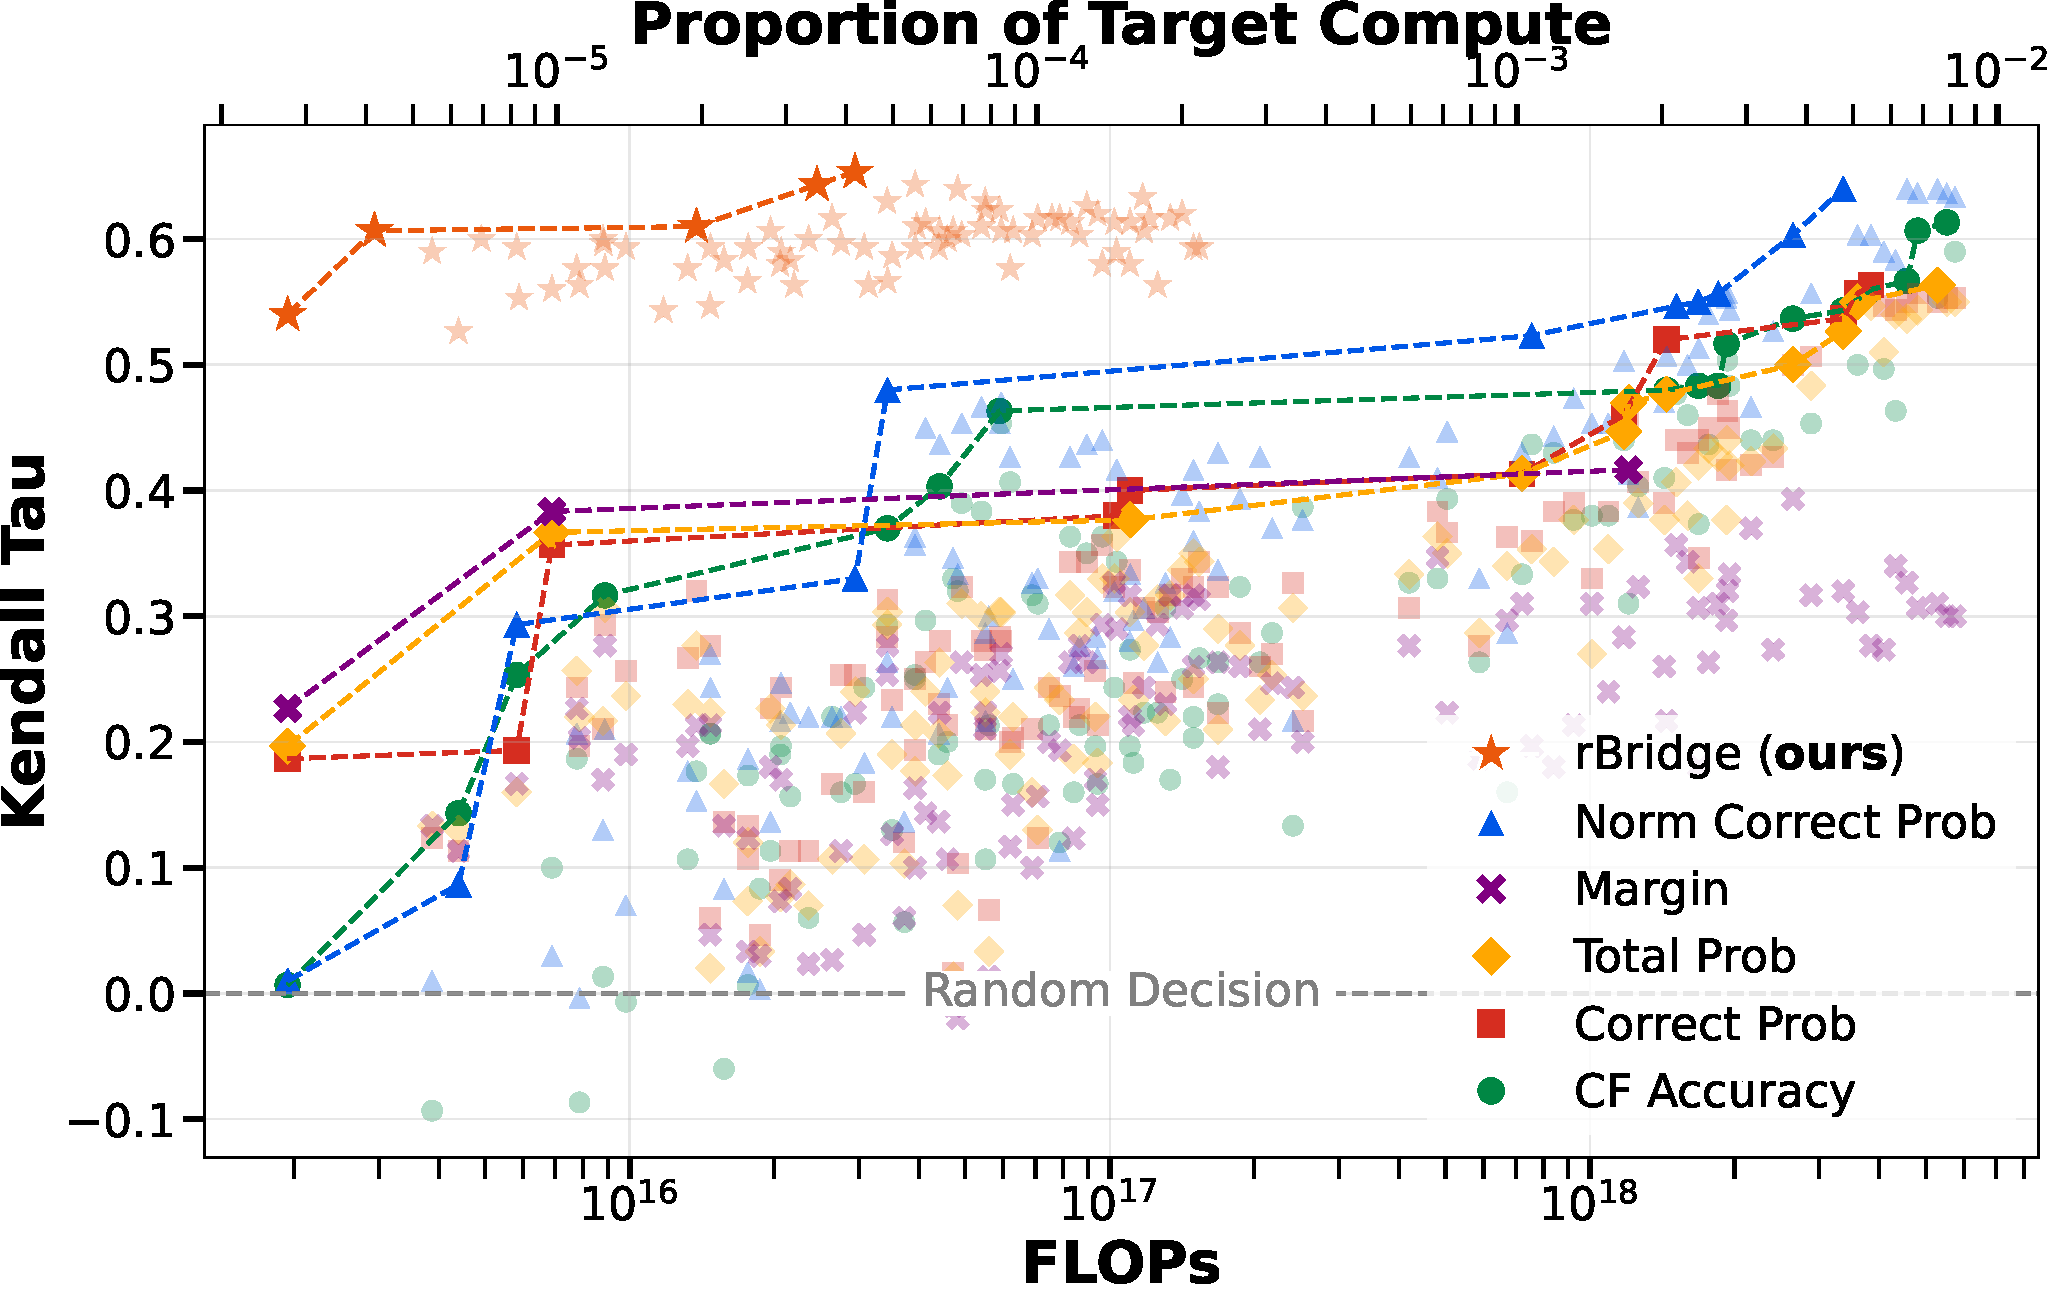
\includegraphics[width=\textwidth]{figs/pareto_kendall.pdf}
        \caption{Kendal Tau results across 3.7 - 97.9M proxy model size, and across intermediary checkpoints.}
        \label{fig:pareto_kendall}
    \end{subfigure}
    \hfill
    \begin{subfigure}[b]{0.497\textwidth}
        \centering
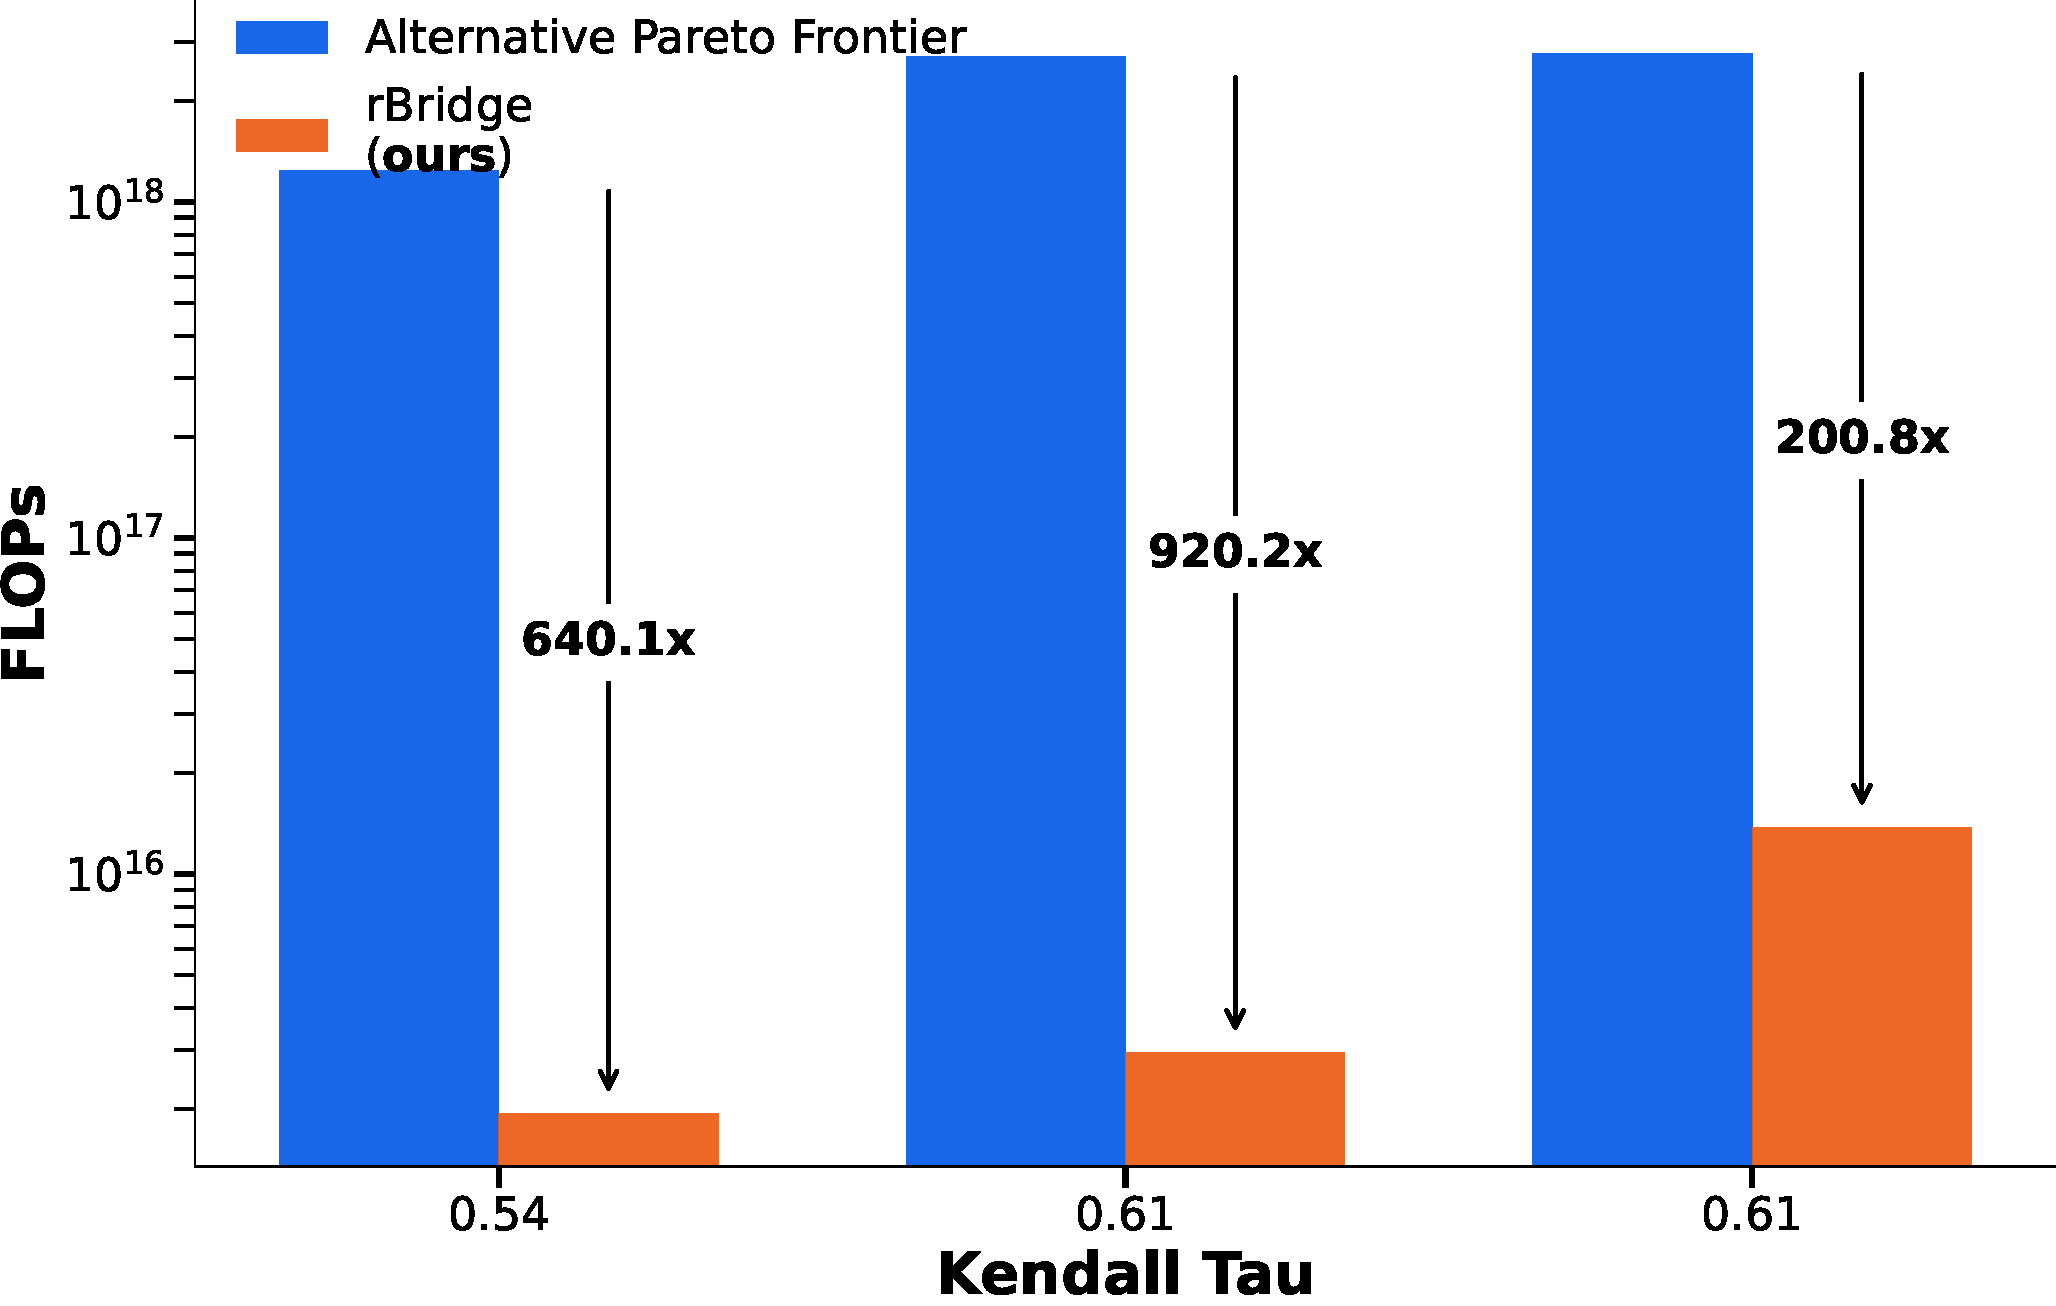
\includegraphics[width=\textwidth]{figs/flops_savings_kendall.pdf}
        \caption{\tsc{rBridge} saves FLOPs by a factor of 200.8$\times$ to 920.2$\times$.}
        \label{fig:flops_kendall}
    \end{subfigure}
    \caption{\tsc{rBridge} improves the pareto frontier in pre-training dataset ranking for 1.2B target model size. Values are averages aggregated across ARC-C and CQA. The two most compute efficient points in \tsc{rBridge}'s pareto frontier is (1) 3.7M model size trained on 87.3M tokens, and (2) 6M model size trained on 81.6M tokens.}
    \label{fig:kendall}
\end{figure}

\section{Proxy Benchmarks are Unreliable} \label{app:proxy_task}

Refer to Fig. \ref{fig:proxytask}.

\begin{figure}[htb]
    \centering
    \begin{subfigure}[b]{0.497\textwidth}
        \centering
        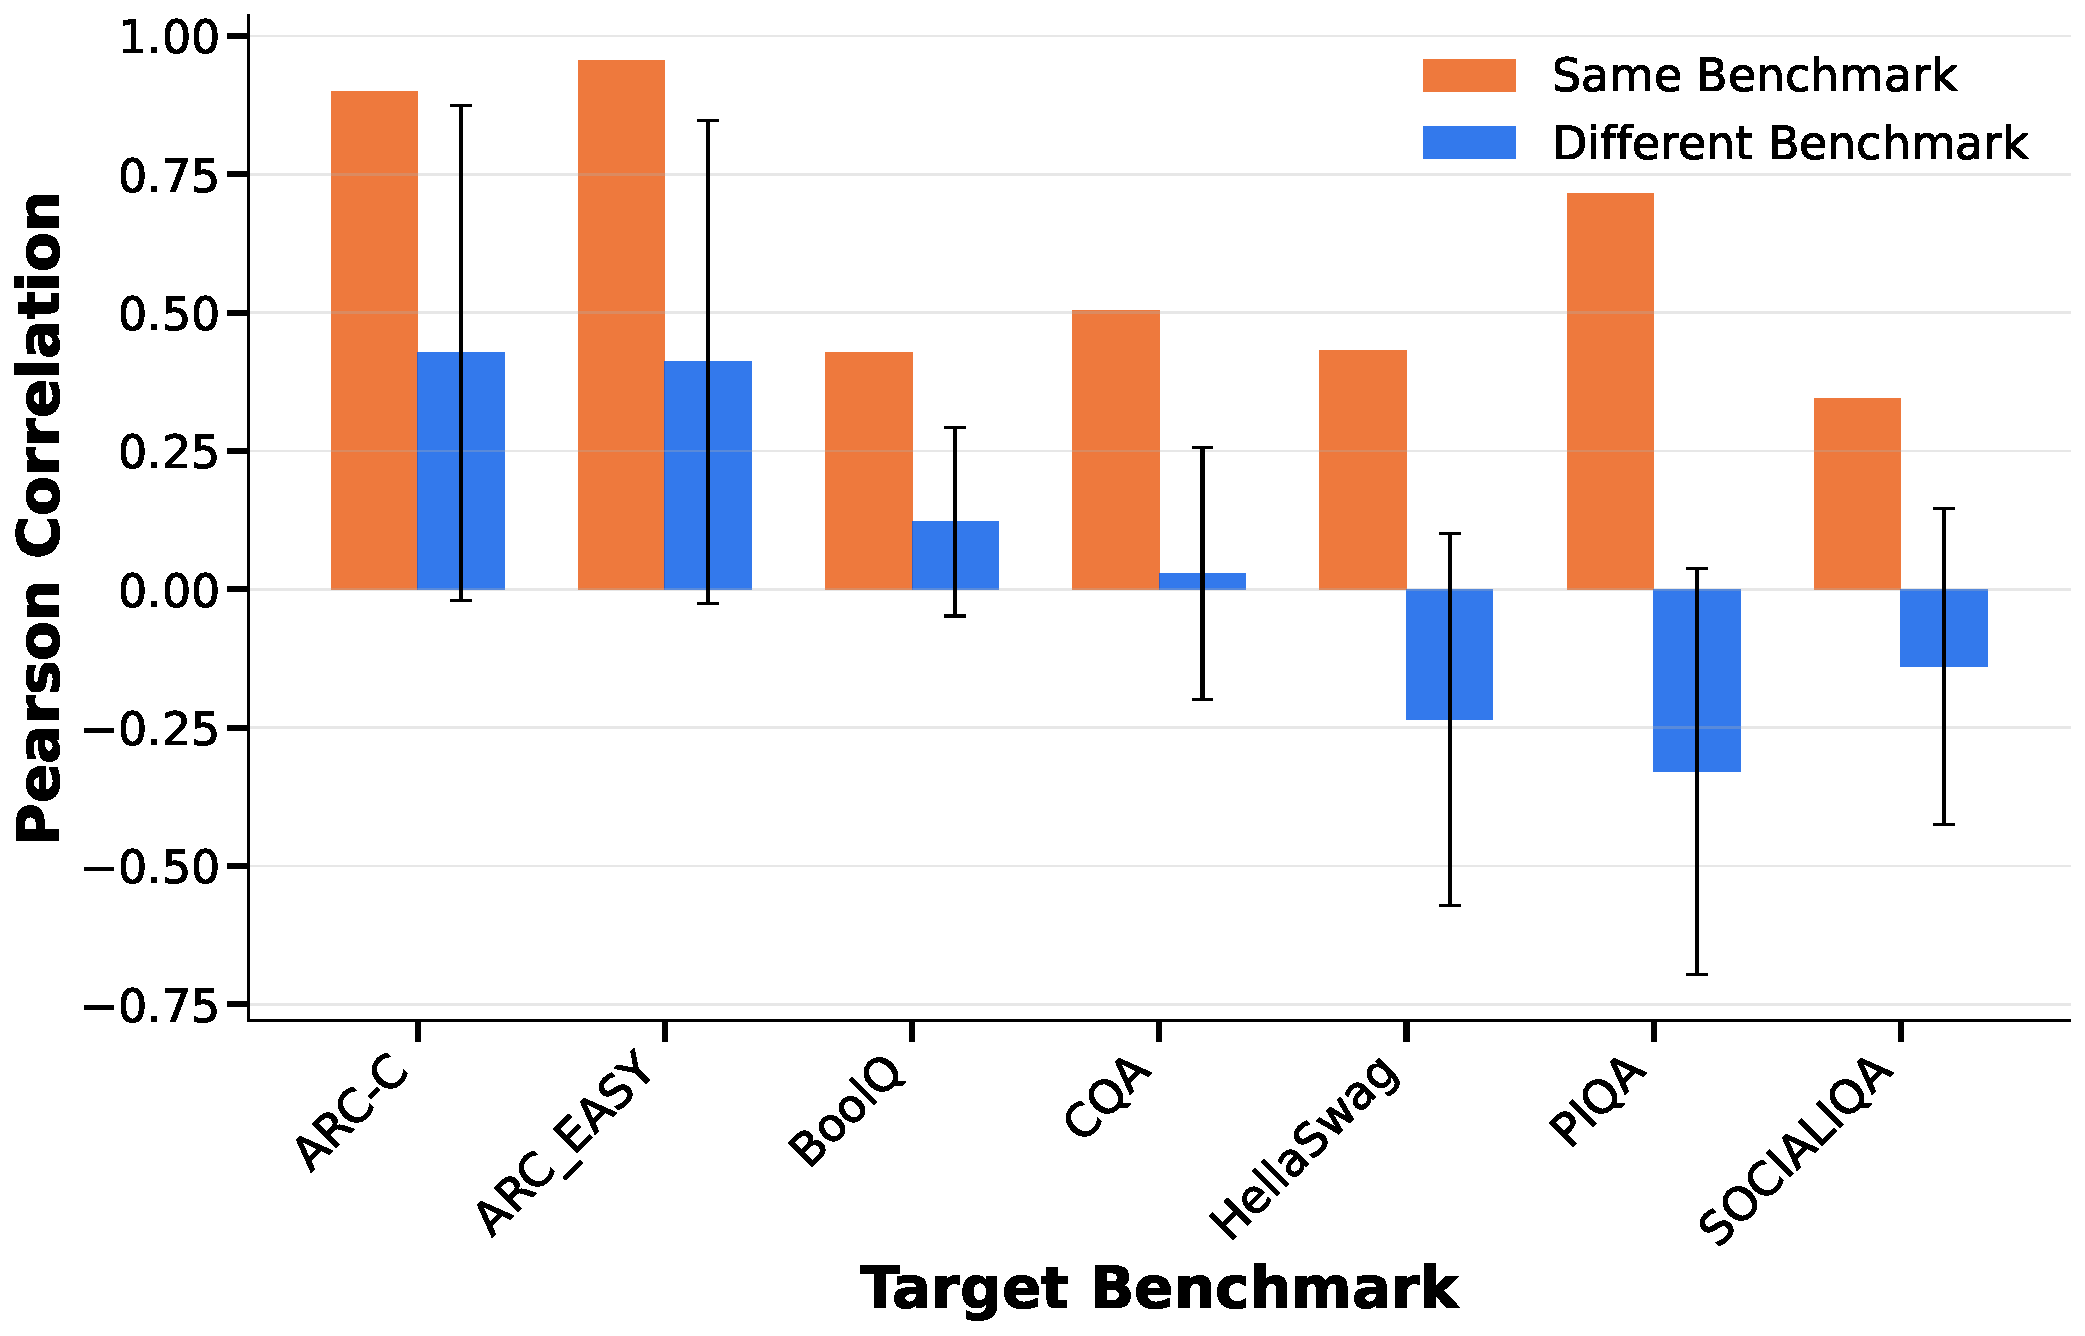
\includegraphics[width=\textwidth]{figs/benchmark_correlation.pdf}
        \label{fig:proxy_corr}
    \end{subfigure}
    \hfill
    \begin{subfigure}[b]{0.497\textwidth}
        \centering
        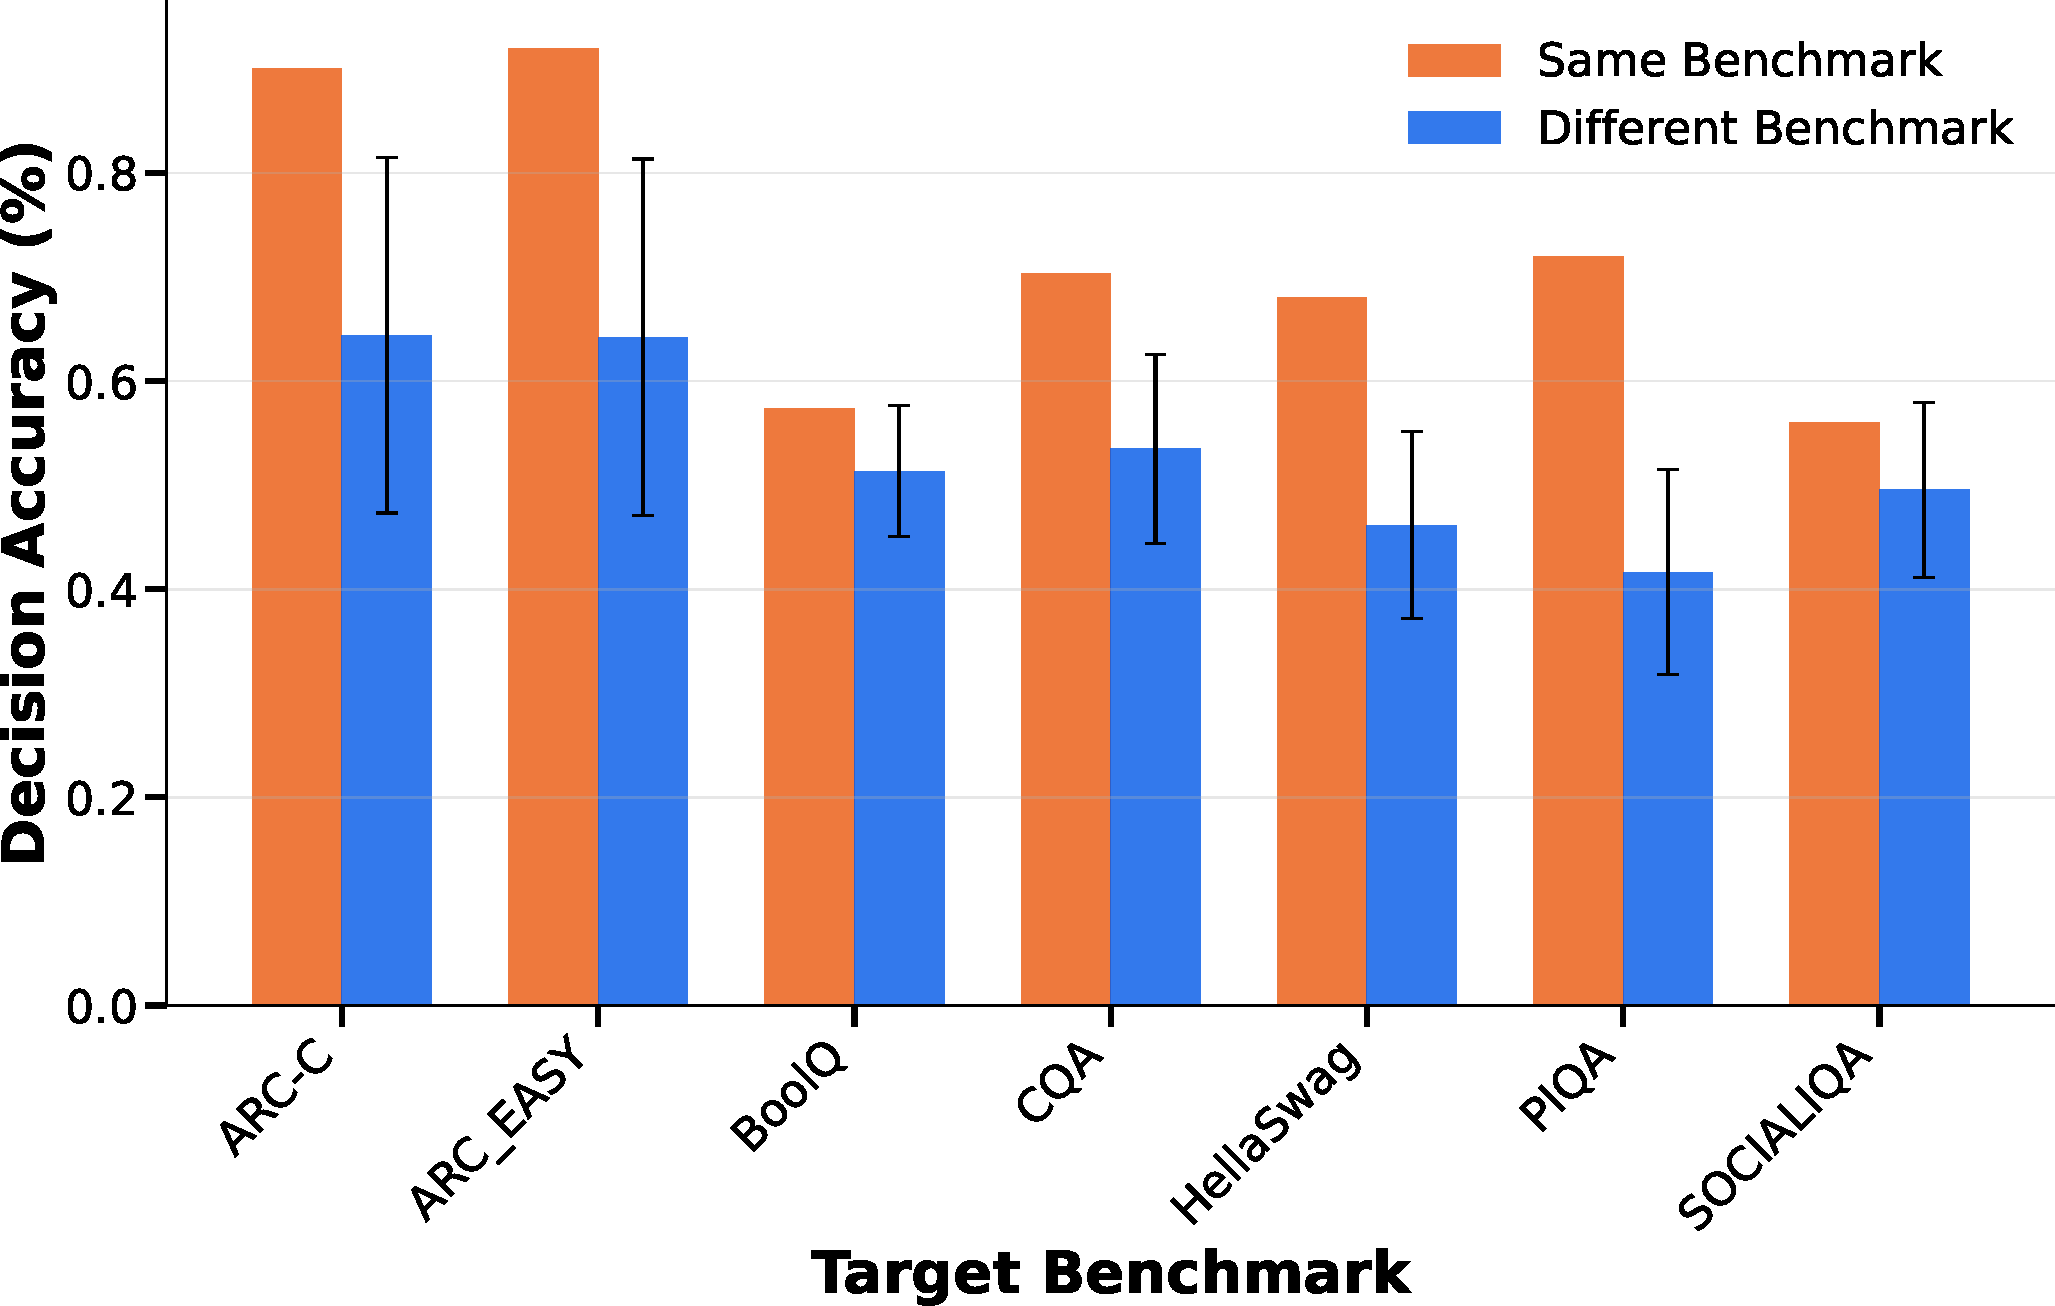
\includegraphics[width=\textwidth]{figs/benchmark_accuracy.pdf}
        \label{fig:proxy_acc}
    \end{subfigure}
    \caption{Correlation and decision accuracy performance using the same benchmark vs. different benchmark on 97.9M $\rightarrow$ 1.2B. Error bars indicate one standard deviation. On average, different benchmarks performs sub-optimally and are noisy.}
    \label{fig:proxytask}
\end{figure}

\section{Attribution} 

We attribute the neural network icon in Fig. \ref{fig:rbridge} as taken from Freepik (flaticon.com). Their guideline indicates that it can be used with attribution.


\end{document}
